\documentclass[10pt]{article}
\usepackage[utf8]{inputenc}
\usepackage[T1]{fontenc}
\usepackage{amsmath}
\usepackage{amsfonts}
\usepackage{amssymb}
\usepackage[version=4]{mhchem}
\usepackage{stmaryrd}
\usepackage{graphicx}
\usepackage[export]{adjustbox}
\graphicspath{ {./images/} }
\usepackage{fancyhdr}
\usepackage{hyperref}
\usepackage{mathrsfs}

\usepackage{multirow}
\usepackage{caption}
\usepackage{enumitem}
\usepackage{subcaption}
\usepackage{pifont}
\usepackage{geometry}
\geometry{left=1.5cm, right=1.5cm, top=2cm, bottom=2cm}
\usepackage{indentfirst}
% Pseudocode Box
\usepackage[ruled,vlined]{algorithm2e}
\setlength{\parindent}{1em}
\setlength{\parskip}{0em}

\newcommand{\norm}[1]{\left#1\right}
\newcommand\course{PHYS3142}  
\newcommand\coursetitle{Computational Methods in Physics}
\newcommand\semester{(Spring 2023)}
\newcommand\hwnumber{3}

%Page setup
\pagestyle{fancy}
\headheight 35pt
\lhead{\course\ \coursetitle\ \semester}
\rhead{
\includegraphics[width=2.5cm]{logo-hkust.png}}
\lfoot{}
\pagenumbering{arabic}
\cfoot{}
\rfoot{\small\thepage}
\headsep 1.2em

\author{\centering LIN, Xuanyu}
\date{\centering \today}


\begin{document}
	\begin{titlepage}
		\begin{center}
			\vspace*{3cm}
			
			\Huge
			\hrulefill
			\vspace{1cm}
			
			\huge
			\textbf{Final Project Report\\}
			\vspace{1cm}
			\textbf{Diffusion-Limited Aggregation}
			\vspace{1cm}
			
			\hrulefill
			
			\vspace{1.5cm}
			\Large
			
			\textbf{LIN, Xuanyu}
			
			\vfill
			
			$\mathscr{COMPUTATIONAL METHOD}$
			
			\vspace{1cm}
			
			\course \ Final Project Report
			
			\vspace{1cm}
			
			
\includegraphics[width=0.4\textwidth]{logo-hkust.png}
			\\
			
			\Large
			
			\today
			
		\end{center}
	\end{titlepage}

\begin{abstract}

In this article, we've discussed about the Diffusion-Limited Aggregation Model in difference circumstances, including the modification of the adjacent sticking probability. The dimension of the clustering is studied via the linear regression. The aggregates formed in DLA have been found to exhibit uniform density with fractal dimension of about 1.7 in two dimensions would increase with the decrease of the sticking probability. Also, the removing range of the particle would definitely affect the clustering result, which would highly affect the programming speed. Different shapes of the initial clustering is also studied. Finally, we discussed about the inconsistant probability to the different directions.

\end{abstract}

\newpage

\tableofcontents

\newpage

\section{Introduction}

\subsection{The History of Diffusion-Limited Aggregation}

Diffusion-limited aggregation (DLA) is a fascinating phenomenon where the particles, due to the Brownian motion, perform a random walk before clustering to each other when they come into contact.\hyperref[ref1]{[1]} It has attracted much attention from physicists, mathematicians, and computer scientists because of its simple model which can explain the formation of complex structures in nature, including fluid dynamics, snowflakes, cracks, lightning etc.

The first known research about DLA was made by physicists Witten T.A. and Sander L.M. in 1981. In their paper, the model is applicable to any aggregation system where diffusion dominates the transport within the system. In computational science, the DLA model has become a popular subject of study due to its simplicity and its ability to generate complex, fractal structures, which was first accomplished in the early 1980s.\hyperref[ref1]{[1]}

\subsection{Different Types of DLA}

Among all the research aspects, there are several major types of the diffusion-limited aggregation models listed as follows:
\begin{enumerate}[itemsep=0pt]
	\item Standard DLA: The simplest type of DLA model, where new particles are released from a point far from the current structure and move randomly in a medium until they come into contact with the existing aggregate.\hyperref[ref2]{[2]}
	\item Multiple-point DLA: Similar to standard DLA, but new particles are released from multiple point sources instead of just one, which results in a more complex and branched fractal structure. Such model is used to model the growth of dendritic structures in metals and alloys.\hyperref[ref3]{[3]}
	\item Stochastic DLA: This model introduces a probabilistic element into the aggregation process, where particles have a chance of bouncing off the aggregate instead of sticking to it. It is used to model the growth of electrochemical deposits and other systems where the aggregation process is influenced by the presence of other particles or fields.\hyperref[ref4]{[4]}
	\item Anisotropic DLA: This model introduces a directional dependence probability of random walk of the particle into the aggregation process. In this model, particles move preferentially in certain directions, resulting in a more elongated or directional fractal structure.\hyperref[ref5]{[5]}
	\item Restricted DLA: This model introduces constraints or obstacles into the medium, such as walls or boundaries, that limit the motion of particles. Restricted DLA is used to model the growth of fractal structures in confined spaces.\hyperref[ref6]{[6]}
\end{enumerate}

It is also worth noticing that the DLA model could be studied via different lattice sites, including square lattice, triangular lattice, hexagonal lattice or circular lattice (allows for more efficient simulations of DLA growth), cubic lattice (in 3-dimensional space), or even random lattice.

\section{Introduction to the Model}

\subsection{Description of the Model}

In this model, we follow the theory proposed by Witten and Sander and later developed by Meakin.\hyperref[ref2]{[2]} A pre-defined lattice structure is constructed, with only the lattice sites of which can be occupied by particles. A seed aggregation is initially placed in the system. Given the radius of the final clustering radius $R_{max}$, particles are added one-by-one to the lattice site at a sufficient distance $R_{max}+5$ from the current aggregation and undergoes a random walk by jumping to one of the neighbor sites. The possible terminal site could be restricted the one of the nearest sites, while the probability $P_{nn}[i]$ moving to either direction could be equal or unequal, which would be further clarified later.

The particle would continues the random walk until it attaches to the cluster or moves too far from the cluster which is $3*CurrentMaxDist$. If the particle moves too far from the cluster, it is deleted from the lattice and started again from a distance closer to the cluster. Only after the previous particle is finally attached to the cluster, is the next particle introduced to the lattice and undergoes the same procedure until the cluster is finally formed.\hyperref[ref7]{[7]}

\newpage

\subsection{Python Code Implementation Structure}

Attach is the structure of the implementation code. The code is used to simulate the DLA model using the Monte-Carlo method.

\begin{algorithm}[H]
	\SetAlgoLined
	\KwIn{TypeOfLatticeSite, InitialCluster, NumOfParticles, (predicted) SimulationRange ($R_{max}$), RemoveRange}
	\KwOut{Image of Formed Cluster, Density Distribution, Calculated Dimension}
	
	\hfill
	
	Construct the lattice site (all lattice to value 0) with sidelength slightly larger than $3*R_{max}$;
	
	Set initial cluster (set the value to 1);
	
	$MaxCurrentRadius \gets CurrentRadius$
	
	\While(\# Count the number of successful simulations){count < NumOfParticles}{
		Randomly generate a particle at radius $MaxCurrentRadius + 5$;
		
		$SimuResult \gets Simulation(Initial\ coordinates)$;
		
		\If{SimuResult > 0}{
			$count \gets count + 1$;
		}
	}
	
	Store\ the\ lattice\ site\ into\ a\ file
	
	Plot\ the\ figure
	
	\hfill
	
	\SetKwFunction{Simulation}{Simulation}
	\SetKwProg{Fn}{Function}{:}{}
	\Fn{Simulation (Initial coordinates)}{
		
		\While{True}{
			$curDist \gets Current\ distance\ to\ the\ center$
			
			\If{SticksToCluster}{
				\If{curDist > SimulationRange}{
					\Return{2};\# Sticks to the cluster exceeding the predicted $R_{max}$, shouldn't occur in the formal experiment
				}
				
				\Else{
					Modify\ the\ $MaxCurrentRadius$\ if\ necessary
				}
			}
		
			\ElseIf(\# Removal of the particle if going too far){
				$curDist > 3*MaxCurrentRadius$
			}{
				Remove\ the\ particle
			}
		
			\Else{
				Randomly\ move\ the\ particle\ to\ one\ of\ the\ vacancies\ adjacent\ to\ it
			}
		}
	}
	\textbf{End Function}
	
	\caption{Basic Algorithm of the Simulation of DLA Model}
\end{algorithm}

\newpage

\section{Simulation of the DLA in Square Lattice}

\subsection{2-Dimensional with Adjacent Sticking}

\subsubsection{Adjacent Sticking \#Prob.=100\% [Task (a)]}

Before the formal experiment, we need to predict the maximum clustering range in order to set the sidelength of the lattice site. We then conducted the pre-experiment with $NumOfParticles=500$, shown in Figure 1 below.

\begin{center}
	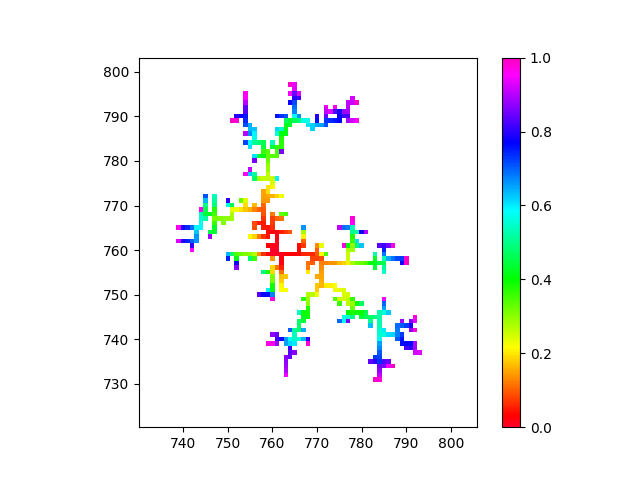
\includegraphics[width=0.4\textwidth]{Figure_1}
	\captionof{figure}{Pre-experiment with Adjacent Sticking \#Prob.=100\%, NumOfParticles=500}
\end{center}

From the figure, we can see that the maximum clustering radius is about 40, so the dimension could be calculated as
$$
Dimension \approx \log_{40}{500} \approx 1.68
$$

Thus, the maximum clustering radius of 10000 particles is predicted as
$$
R_{max} \approx 10000^{\frac{1}{1.68}} \approx 237
$$

In the formal simulation of 10000 particles, we set the maximum clustering range to be 250, slightly larger than the approximation to avoid randomness, according to the pre-experiment. Thus, the sidelength of the lattice site is set to be $2*(3*R_{max}+10)=1520$, the initial point is set at $(760,760)$.

The base case with nearest sticking probability $P_{nn}=100\%$ is simulated via the python file \texttt{v2.2\_Base\_Case\_Square.py}. The Figure 2 below is one of the 20 simulation results that is used later to calculate the fractional dimension. All the 20 simulation results are stored inside the folder \texttt{Base\_Case}.

Note that we've also calculated the (successfully) clustering rate, which is defined by the ratio of the number of successfully-clustering particles (10000) and the total number of the particles being simulated, including those that are removed. e.g. the attached figure has a clustering rate=74.45\%. The clustering rate can be seen in the file names.

The 20 clustering rates are listed in increasing order below, which could be reached via the file names: 71.80\%, 72.20\%, 73.27\%, 73.37\%, 73.73\%, 73.89\%, 74.22\%, 74.45\%, 74.54\%, 74.58\%, 74.92\%, 74.99\%, 75.53\%, 75.71\%, 76.05\%, 76.40\%, 77.23\%, 77.45\%, 78.62\%, 79.02\%, with an average of $(75.10\pm 1.89)\%$.

\begin{center}
	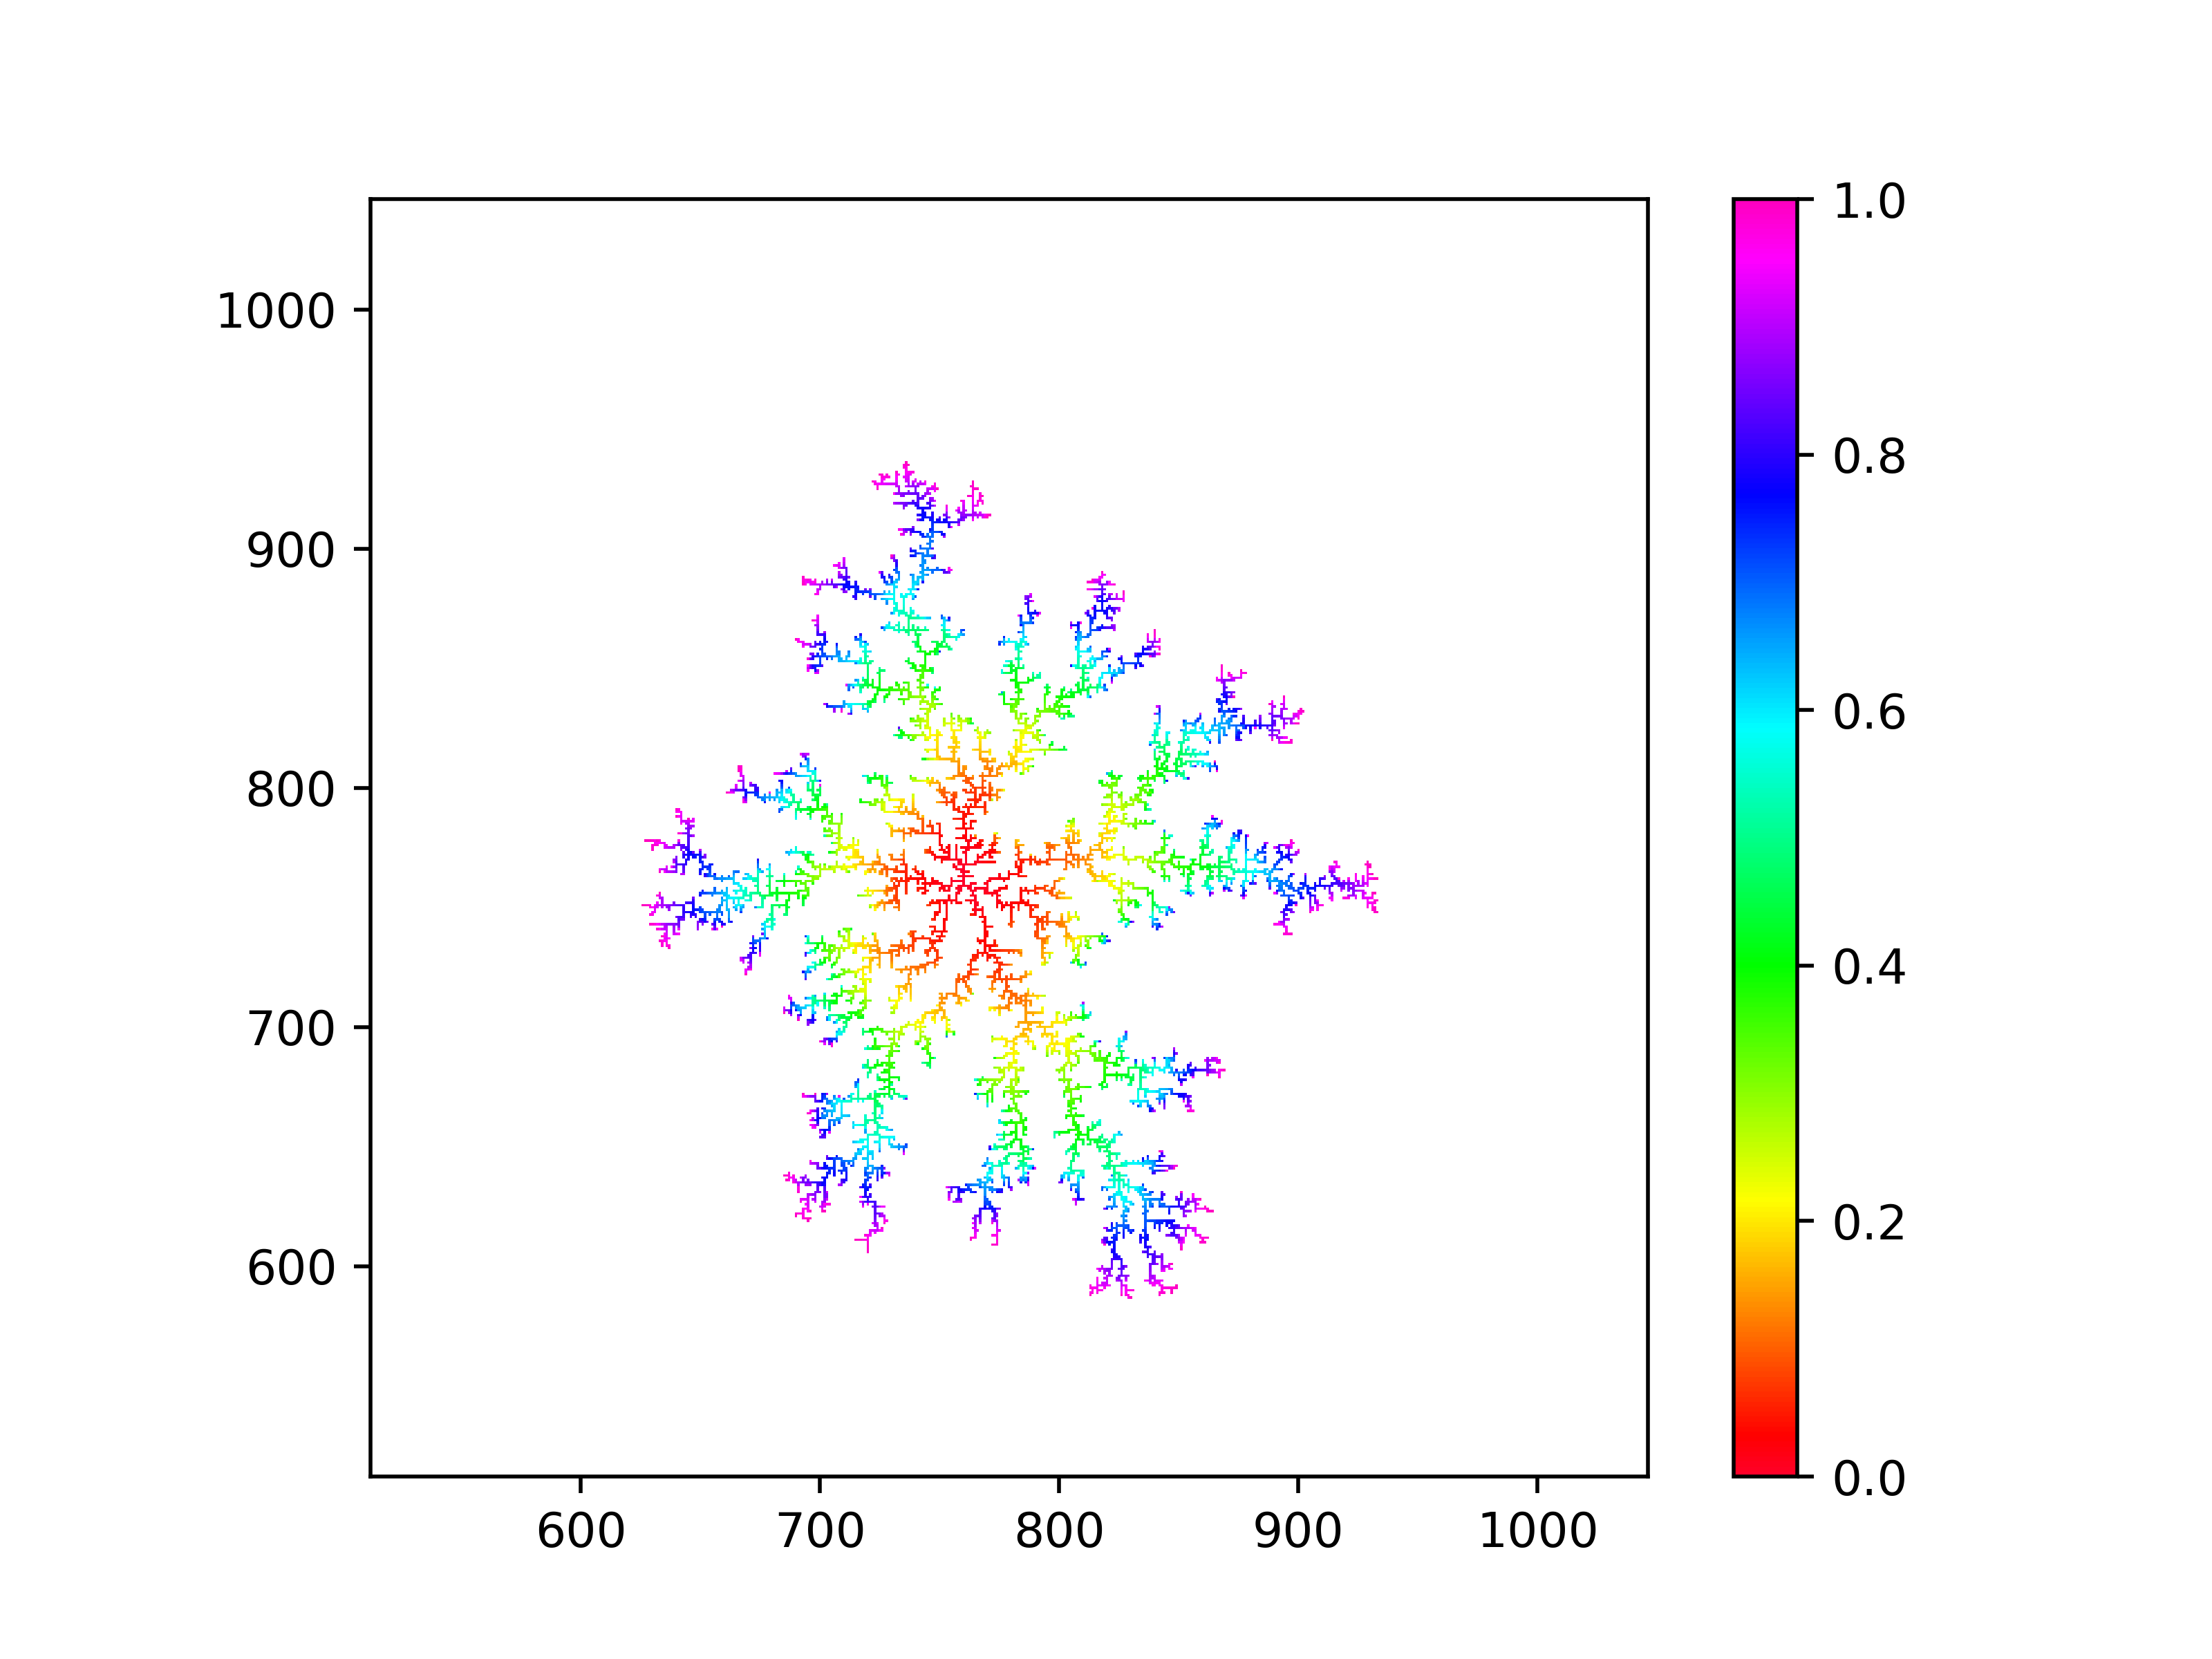
\includegraphics[width=0.4\textwidth]{Figure_2}
	\captionof{figure}{Adjacent Sticking \#Prob.=100\%, clustering rate=74.45\% [Task (a)]}
\end{center}

\subsubsection{Adjacent Sticking \#Prob.=30\% [Task (b)]}

This simulation is similar to the previous section. We simply change the checking function $SticksToCluster$ to a probabilistic event. Only when the adjacent is filled and the newly-generated random number is less than 0.3, will it be regarded as an aggregation.

Similarly, the pre-experiment tells us that the dimension is similar to the previous section, so we don't need to change the maximum clustering range, the lattice range and the initial point, which is at $(760,760)$.

Figure 3 below shows one of the 20 simulation results with nearest sticking probability $P_{nn}=30\%$, which is simulated via the python file \texttt{v2.2\_Modified\_Prob=0.3.py} inside the folder \texttt{Modified\_Prob}.

The 20 clustering rates are listed in increasing order below, which could be reached via the file names: 68.80\%, 69.66\%, 69.87\%, 70.22\%, 70.33\%, 70.38\%, 70.81\%, 72.64\%, 72.65\%, 72.83\%, 72.97\%, 73.64\%, 73.77\%, 74.09\%, 74.37\%, 74.77\%, 74.81\%, 75.23\%, 75.33\%, 75.75\%, with an average of $(72.69\pm 2.17)\%$.

We can see that the average clustering rate is about 2.5\% smaller than the previous one with adjacent sticking \#Prob.=100\%, which is consistent with the intuition.

\begin{center}
	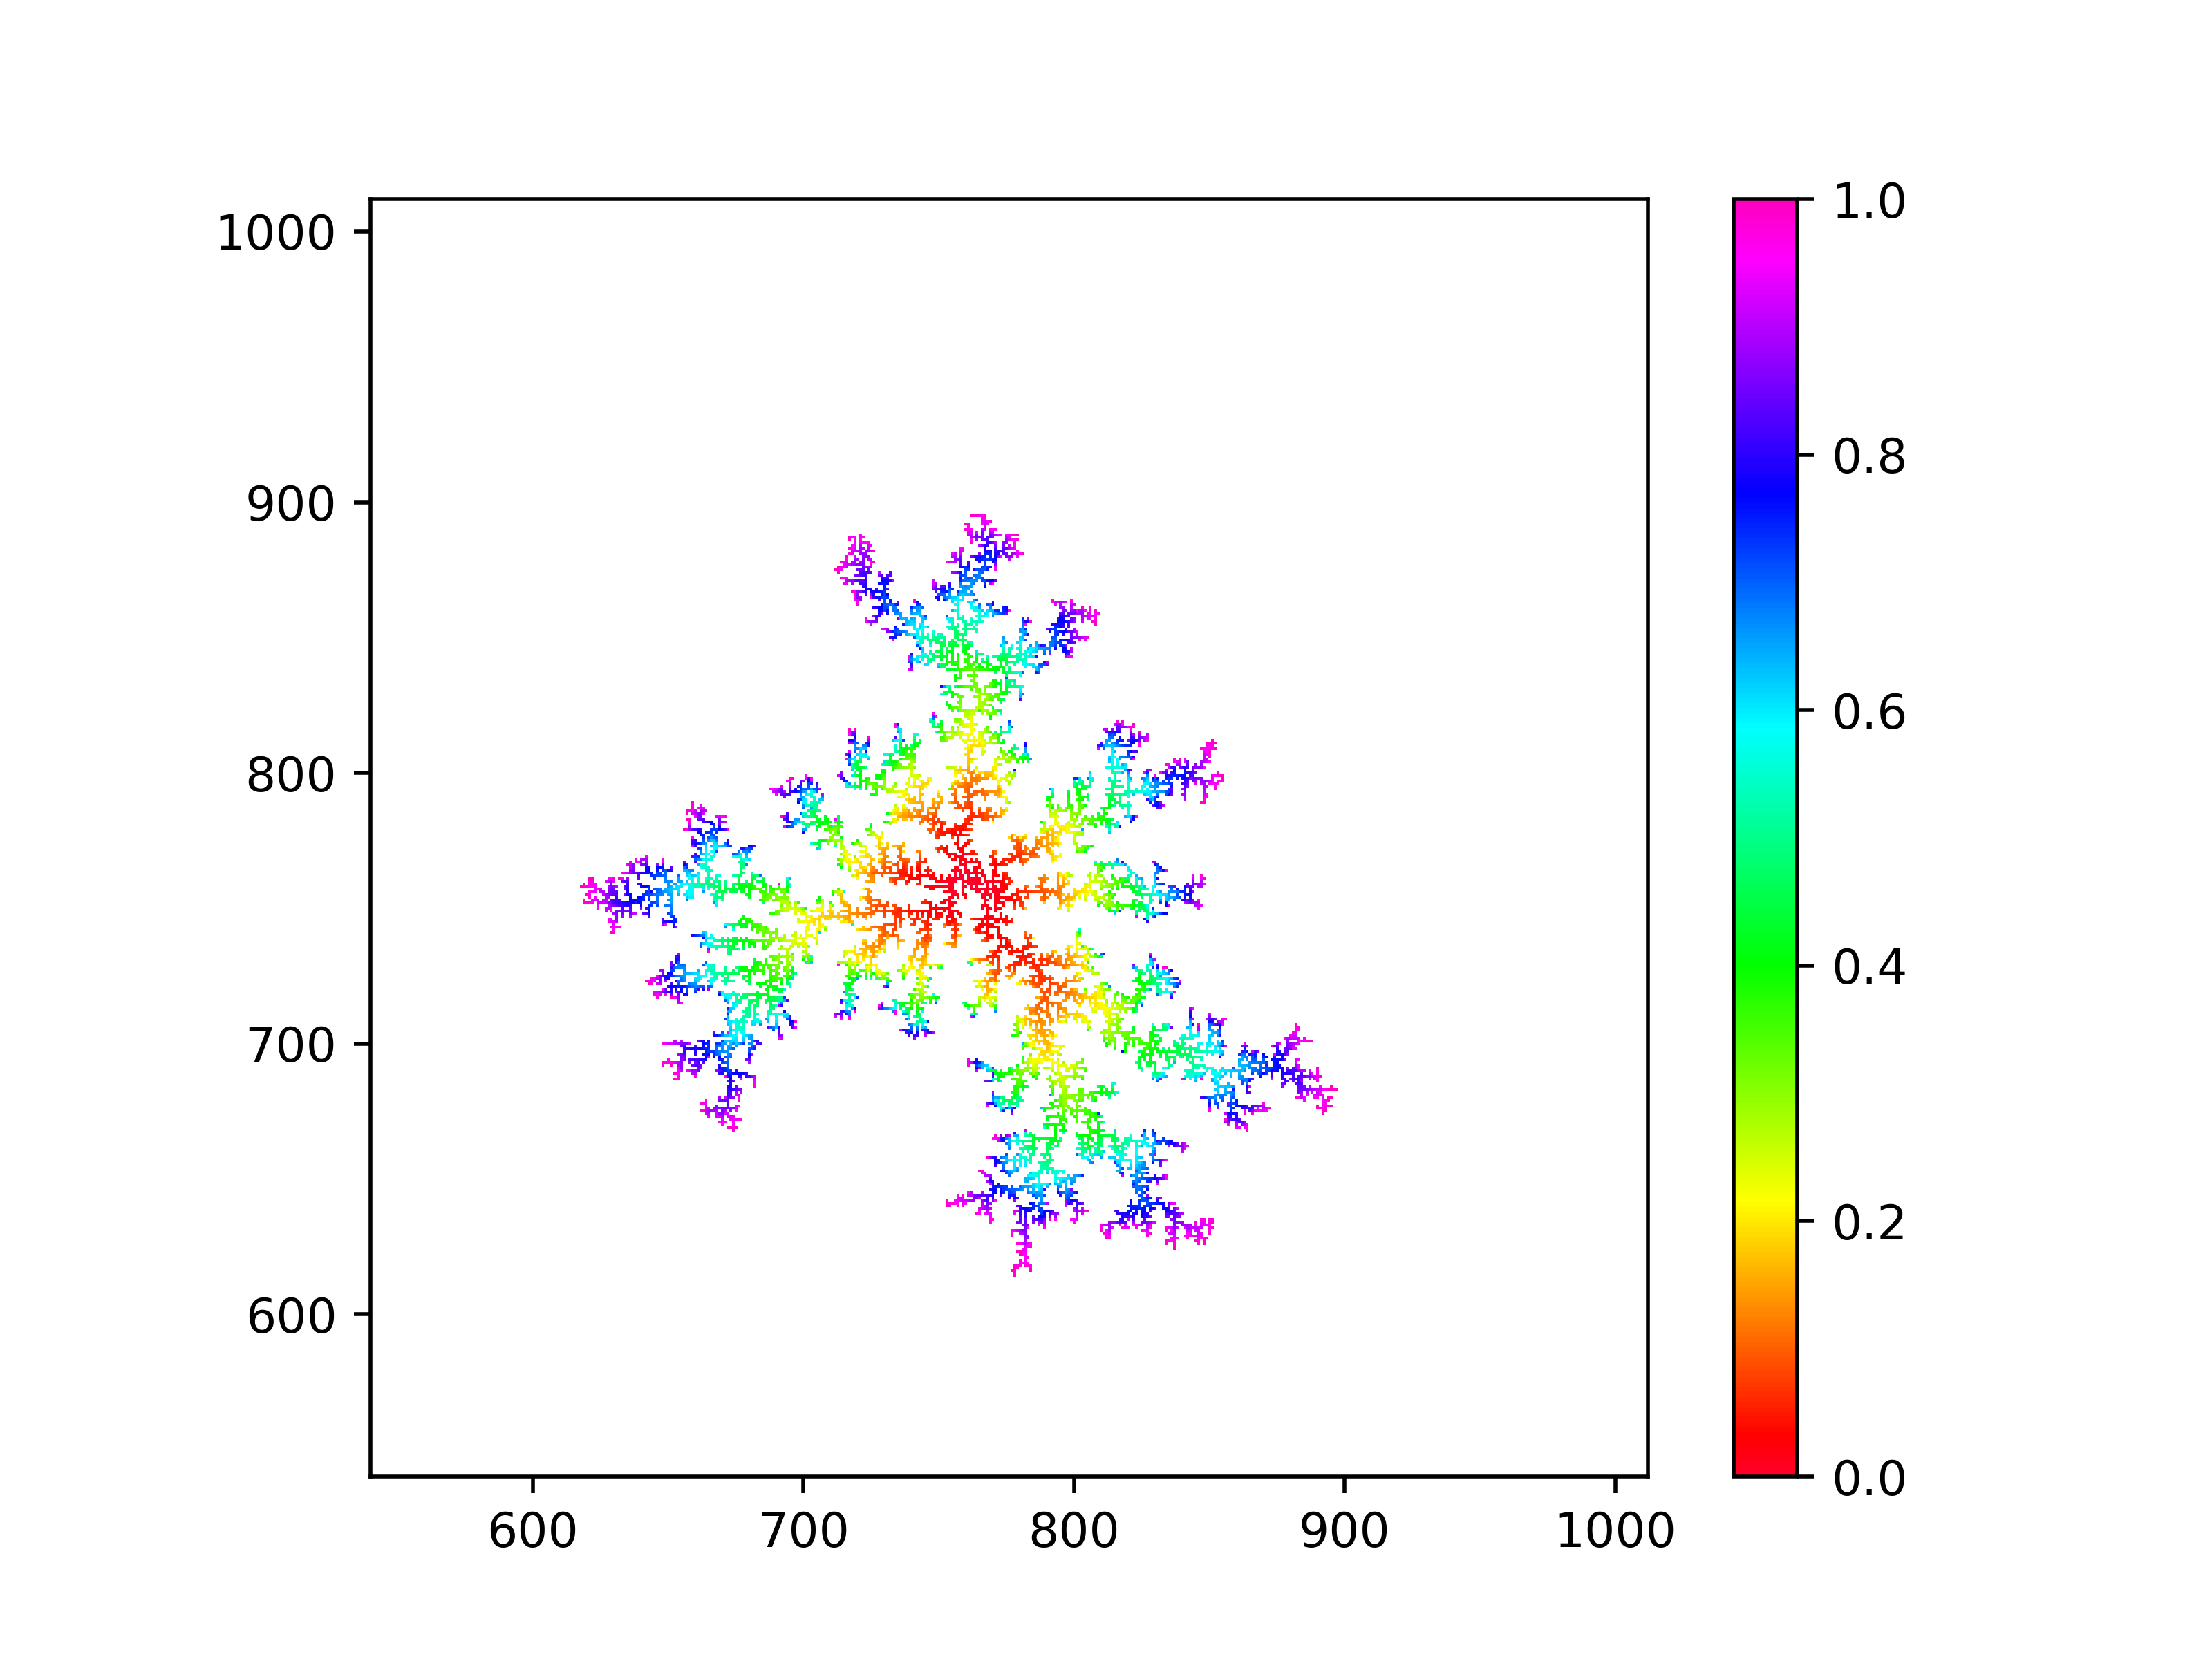
\includegraphics[width=0.4\textwidth]{Figure_3}
	\captionof{figure}{Adjacent Sticking \#Prob.=30\%, clustering rate=70.38\% [Task (b)]}
\end{center}

\subsubsection{Density Distribution \& Dimension Analysis [Task (c)(d)]}

To analyze the density distribution, we first calculate the density function $C(r)$ which represents the number of particles at distance $r$ from the reference particle for the all particles in the cluster and then normalizes it using the total number of particles and the corresponding volume between two spheres of radius $(r-\delta r)$ and $(r+\delta r)$ respectively. The algorithm is shown below.

We first derive the formula about the fractional dimension as below. Suppose the cumulative number of clustering points within radius $r$ can be represented as
$$
S(r) = A r^{\text{dim}}
$$

where dim refers to the dimension of the final cluster with some constant A.

According to the definition\hyperref[ref7]{[7]},
$$
\begin{aligned}
	C(r) \cdot 2 \pi r \mathrm{d} r = \mathrm{d} S &\implies C(r) = \frac{1}{2 \pi r}\frac{\mathrm{d} S}{\mathrm{d} r} = \frac{A \cdot \text{dim}}{2 \pi} r^{\mathrm{dim} - 2}\\
	&\implies \ln C(r) = (\mathrm{dim} - 2) \cdot \ln r + \text{Constant}
\end{aligned}
$$

When defining the density function as $C(r) = r^{-\alpha}$ specified in the description\hyperref[ref7]{[7]}, we have
$$
\alpha = 2-\text{dim} \implies \text{Fractional Dimension } D = d-\alpha = 2-(2-\text{dim}) = \text{dim}
$$

which fits the theory correctly.

In this section, we perform the two algorithms below to generate both cumulative density function $S(r)$ and edge density function $C(r)$. We take the cumulative density function $S(r)$ as an example, as we can simply replace the variable $density\_distribution$ with a subtraction to obtain $C(r)$.

\begin{algorithm}[H]
	\SetAlgoLined
	\KwIn{The Files of Clustering Result}
	\KwOut{Fitting Result, Calculated Dimension}
	
	\hfill
	
	Change directory to current file;
	
	Define number of files as \texttt{file\_number};
	
	Initialize empty array \texttt{data} sized (\texttt{file\_number, Array\_Size, Array\_Size});
	
	\hfill
	
	\For{All files}{
		\texttt{data[i]} $\gets$ \texttt{file\_list[i]}
	}

	\hfill
	
	\SetKwFunction{pointsWithinRadius}{points\_within\_radius}
	\SetKwProg{Fn}{Function}{:}{}
	\Fn(\# Count the number of points within a given radius){points\_within\_radius (\texttt{distances, radius})}{
		\Return{np.sum(distances <= radius)}
	}
	\textbf{End Function}

	\hfill
	
	\For{i < \texttt{file\_number}}{
		Extract the positive data into 2D array \texttt{positive\_data}
		
		Find the center of the array and calculate the distances from the center for points stored in \texttt{positive\_data}
		
		Calculate the cumulative number of clustered points by
		
		$density\_distribution \gets [points\_within\_radius(distances, r)$ for $r$ in range($max\_radius+1-50$)]
		
		Calculate the logarithm of $density\_distribution$
		
		Do the linear regression using $np.polyfit$ and store the slope
	}
	
	Calculate the average and the standard deviationof the stored slope
	
	\caption{Algorithm of Fitting the Cumulative Density Function $S(r)$ (similar for $C(r)$)}
\end{algorithm}

The plotting of density function $\ln C(r) \text{ vs } \ln r$ is shown in Figure 4, for adjacent sticking probability being 100\% and 30\% respectively, which are simulated via the python file \texttt{Edge\_distribution.py} inside the two folders \texttt{Base\_Case} \& \texttt{Modified\_Prob}.

\begin{figure}[h]
	\centering
	\begin{subfigure}[b]{0.3\textwidth}
		\centering
		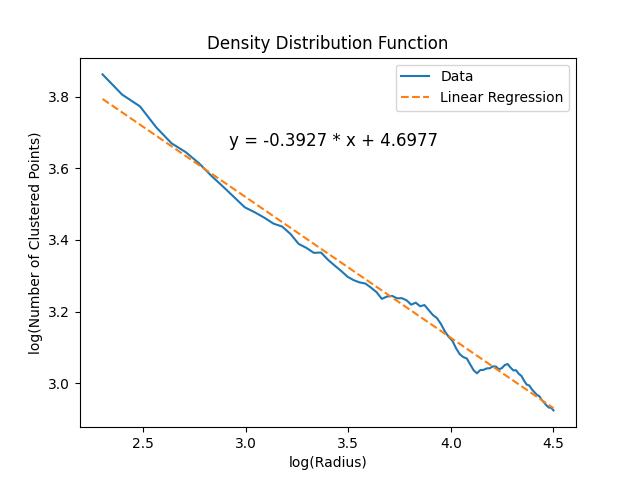
\includegraphics[width=\textwidth]{Figure_4}
		\caption{Density Function $\ln C(r) \text{ vs } \ln r$ for adjacent sticking probability = 100\%}
	\end{subfigure}
	% \hfill
	\begin{subfigure}[b]{0.3\textwidth}
		\centering
		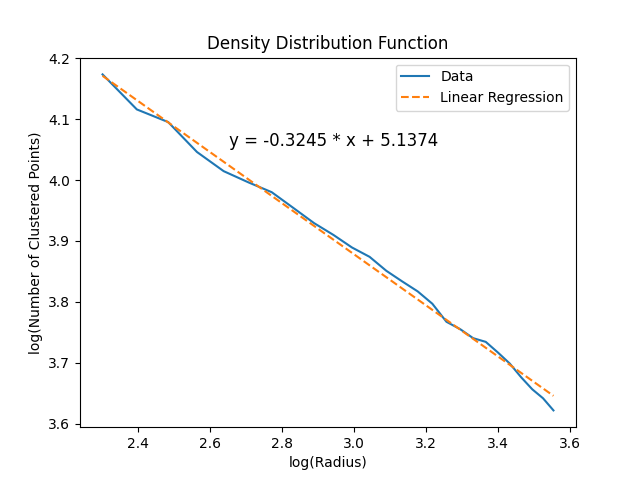
\includegraphics[width=\textwidth]{Figure_5}
		\caption{Density Function $\ln C(r) \text{ vs } \ln r$ for adjacent sticking probability = 30\%}
	\end{subfigure}
	\caption{$\ln C(r) \text{ vs } \ln r$ for Different Adjacent Sticking Probability}
\end{figure}

Notice that, due to the insufficient number of points within one "slide", the data are very fragile, the fitting result is not good enough for analyzing the tiny difference between the two dimensions.

We then consider to use the \textbf{same set of data} to replot the figure in a different way. According to the discussion above, we've already proved the sameness of the cumulative density function $S(r)$ and the edge density function $C(r)$, where the power of the cumulative density function $S(r)$ is just the same as the dimension.

Thus, we manage to directly plot $\ln S(r) \text{ vs } \ln r$ to obtain the dimension as below.

\newpage

\begin{figure}[h]
	\centering
	\begin{subfigure}[b]{0.3\textwidth}
		\centering
		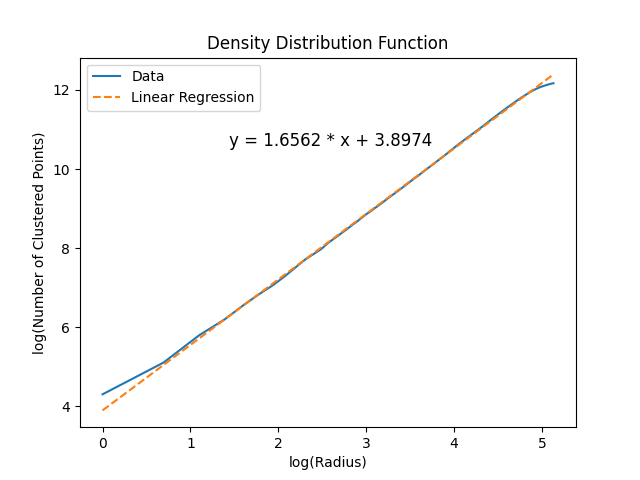
\includegraphics[width=\textwidth]{Figure_6}
		\caption{Density Function $\ln S(r) \text{ vs } \ln r$ for adjacent sticking probability = 100\%}
	\end{subfigure}
	% \hfill
	\begin{subfigure}[b]{0.3\textwidth}
		\centering
		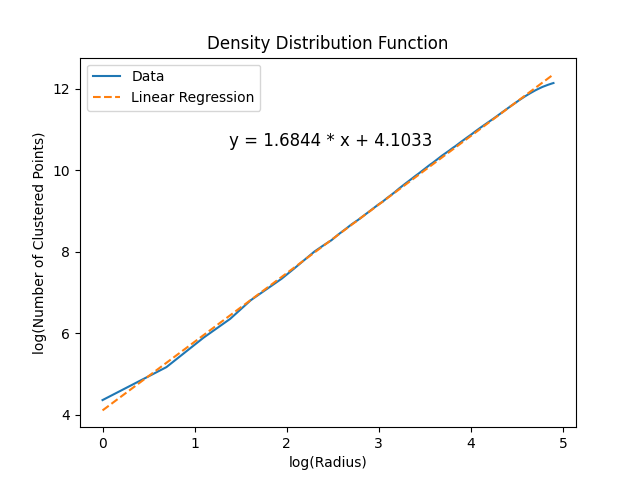
\includegraphics[width=\textwidth]{Figure_7}
		\caption{Density Function $\ln S(r) \text{ vs } \ln r$ for adjacent sticking probability = 30\%}
	\end{subfigure}
	\caption{$\ln S(r) \text{ vs } \ln r$ for Different Adjacent Sticking Probability}
\end{figure}

The plots of $\ln S(r) \text{ vs } \ln r$ are obviously more stable and accurate than the plot of the $\ln C(r) \text{ vs } \ln r$. Thus, we'll use this point of view to discuss the dimensions from now on.

The fitting results together with the dimensions obtained from both $C(r)$ \& $S(r)$ are listed in the Table 1 below.
\begin{center}
	\begin{table}[h]
	\begin{tabular}{|c|c|c|c|c|c|}
		\hline
		\multirow{2}{*}{\shortstack{Adjacent Sticking\\Probability}} & \multirow{2}{*}{\shortstack{Slope Obtained\\from $C(r)$}} & \multirow{2}{*}{Value of $\alpha$} & \multirow{2}{*}{\shortstack{Dimension\\Obtained from $C(r)$}} & \multirow{2}{*}{\shortstack{Slope Obtained\\from $S(r)$}} & \multirow{2}{*}{\shortstack{Dimension\\Obtained from $S(r)$}} \\
		& & & & & \\
		\hline
		1 & $-0.39\pm 0.03$ & -0.39 & 1.61 & $1.656\pm 0.005$ & 1.656 \\
		\hline
		0.3 & $-0.32\pm 0.04$ & -0.32 & 1.68 & $1.684\pm 0.003$ & 1.684 \\
		\hline
	\end{tabular}
	\caption{Dimensions Obtained from both $C(r)$ \& $S(r)$}
	\end{table}
\end{center}

\subsubsection{Dimension Analysis with the Change of Adjacent Sticking Probability}

We can see from the previous discussion that with the increase of sticking probability, the dimension is decreasing in a slow rate.

One possible explanation for this trend is that the adjacent sticking probability affects the way in which particles are added to the growing fractal structure. When particles stick to adjacent particles with a high probability, they are more likely to attach to existing clusters rather than forming new ones. This can lead to a more decentralized growth pattern, which can result in a fractal structure that is more spread out and has a lower dimension.

Another possible explanation is that the adjacent sticking probability promotes the formation of compact clusters of particles, which can lead to a decrease in the overall fractal dimension. When particles stick to adjacent particles with a high probability, they are more likely to form clusters that are tightly packed in the outside area in a small range, which can result in a fractal structure that is less complex and has a lower dimension.

Overall, the observation that the dimension of the DLA fractal structure decreases with an increase in the adjacent sticking probability is an interesting result. Further analysis and investigation of the underlying mechanisms behind this trend could lead to a better understanding of the factors that influence the formation and properties of fractal structures in general. Additionally, this information could be useful in designing and optimizing fractal-based systems, such as in the development of new materials or in the study of natural phenomena.

\subsubsection{Discussion about the Removing Range}

We then consider the impact of the removing range of the particle when it's going too far. In the Final Project description\hyperref[ref7]{[7]}, the removing rage is restricted to be three times of the current maximum clustering radius. In this section, we'll change such parameter to discover its impact. The original simulations results are stored inside the folder \texttt{Other\_Simulation/Effect\_R\_remove}.

Below in the Figure 6 shows the 8 samples of the clustering result, with the remove range being from of the same multiple as the current maximum radius to three times of it.

\newpage

\begin{figure}[h]
	\centering
	\begin{subfigure}[b]{0.2\textwidth}
		\centering
		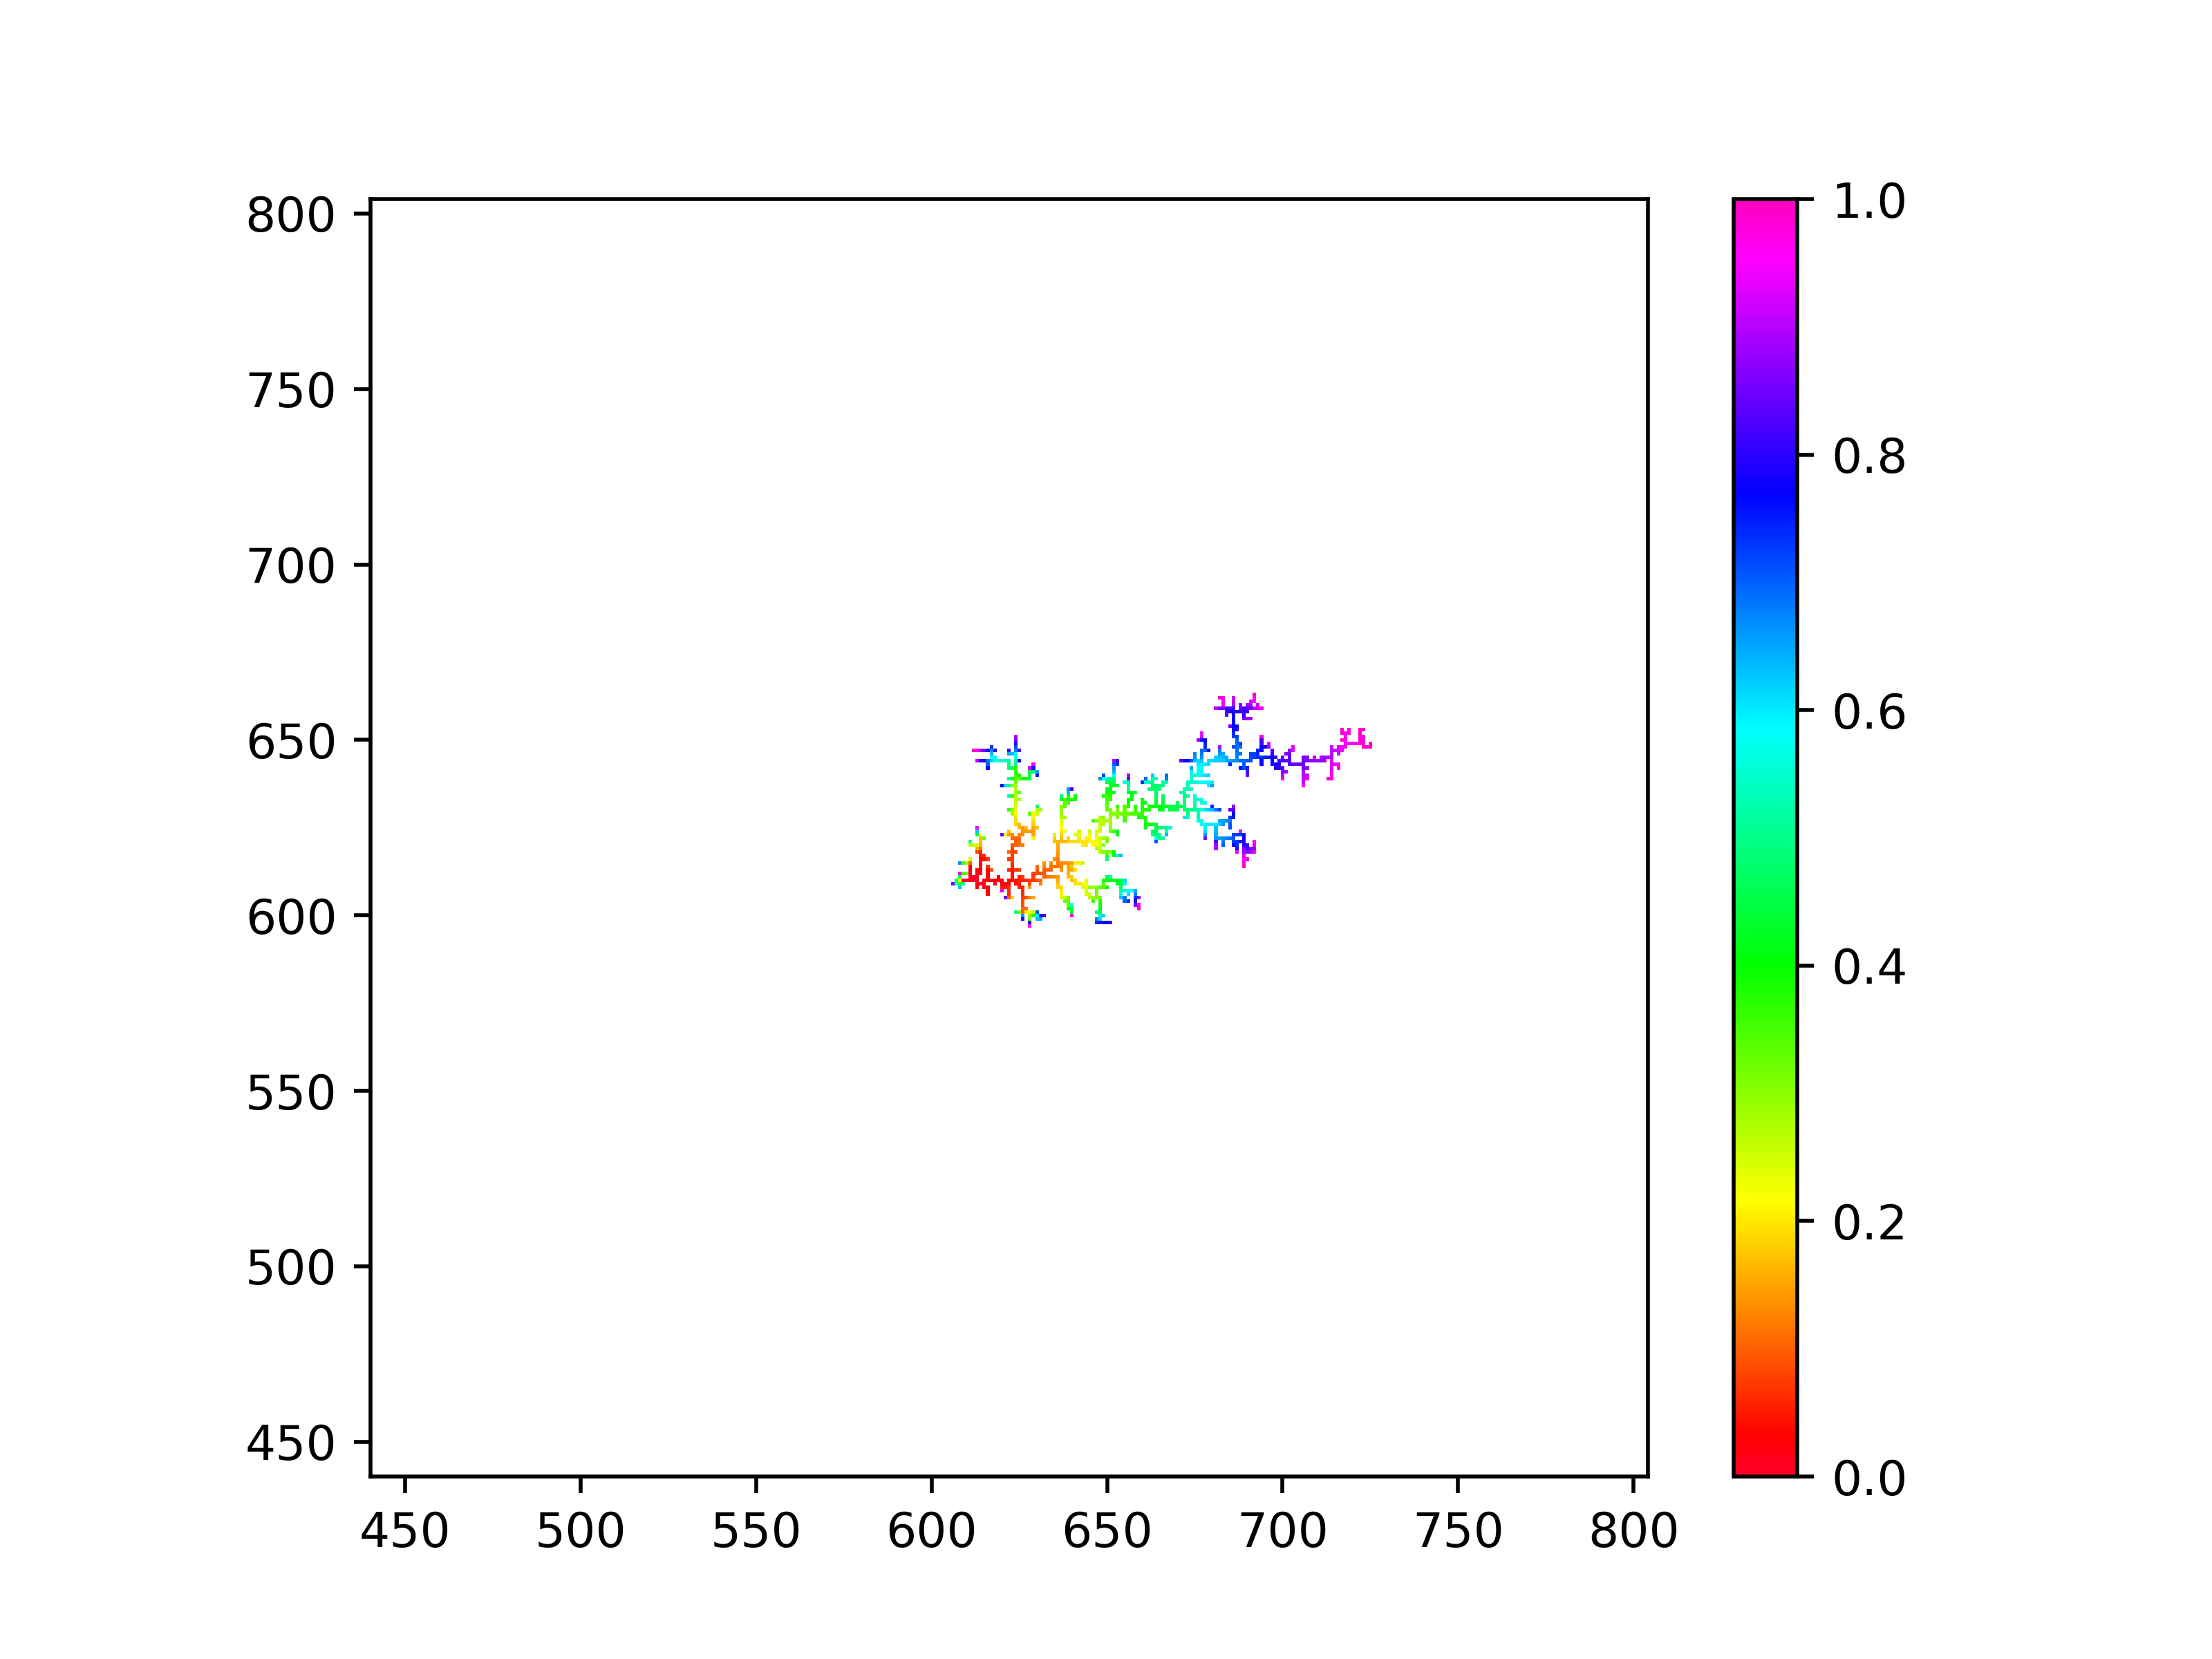
\includegraphics[width=\textwidth]{Figure_10_1}
		\caption{C=1.84\% Rmv=1}
	\end{subfigure}
	\hfill
	\begin{subfigure}[b]{0.2\textwidth}
		\centering
		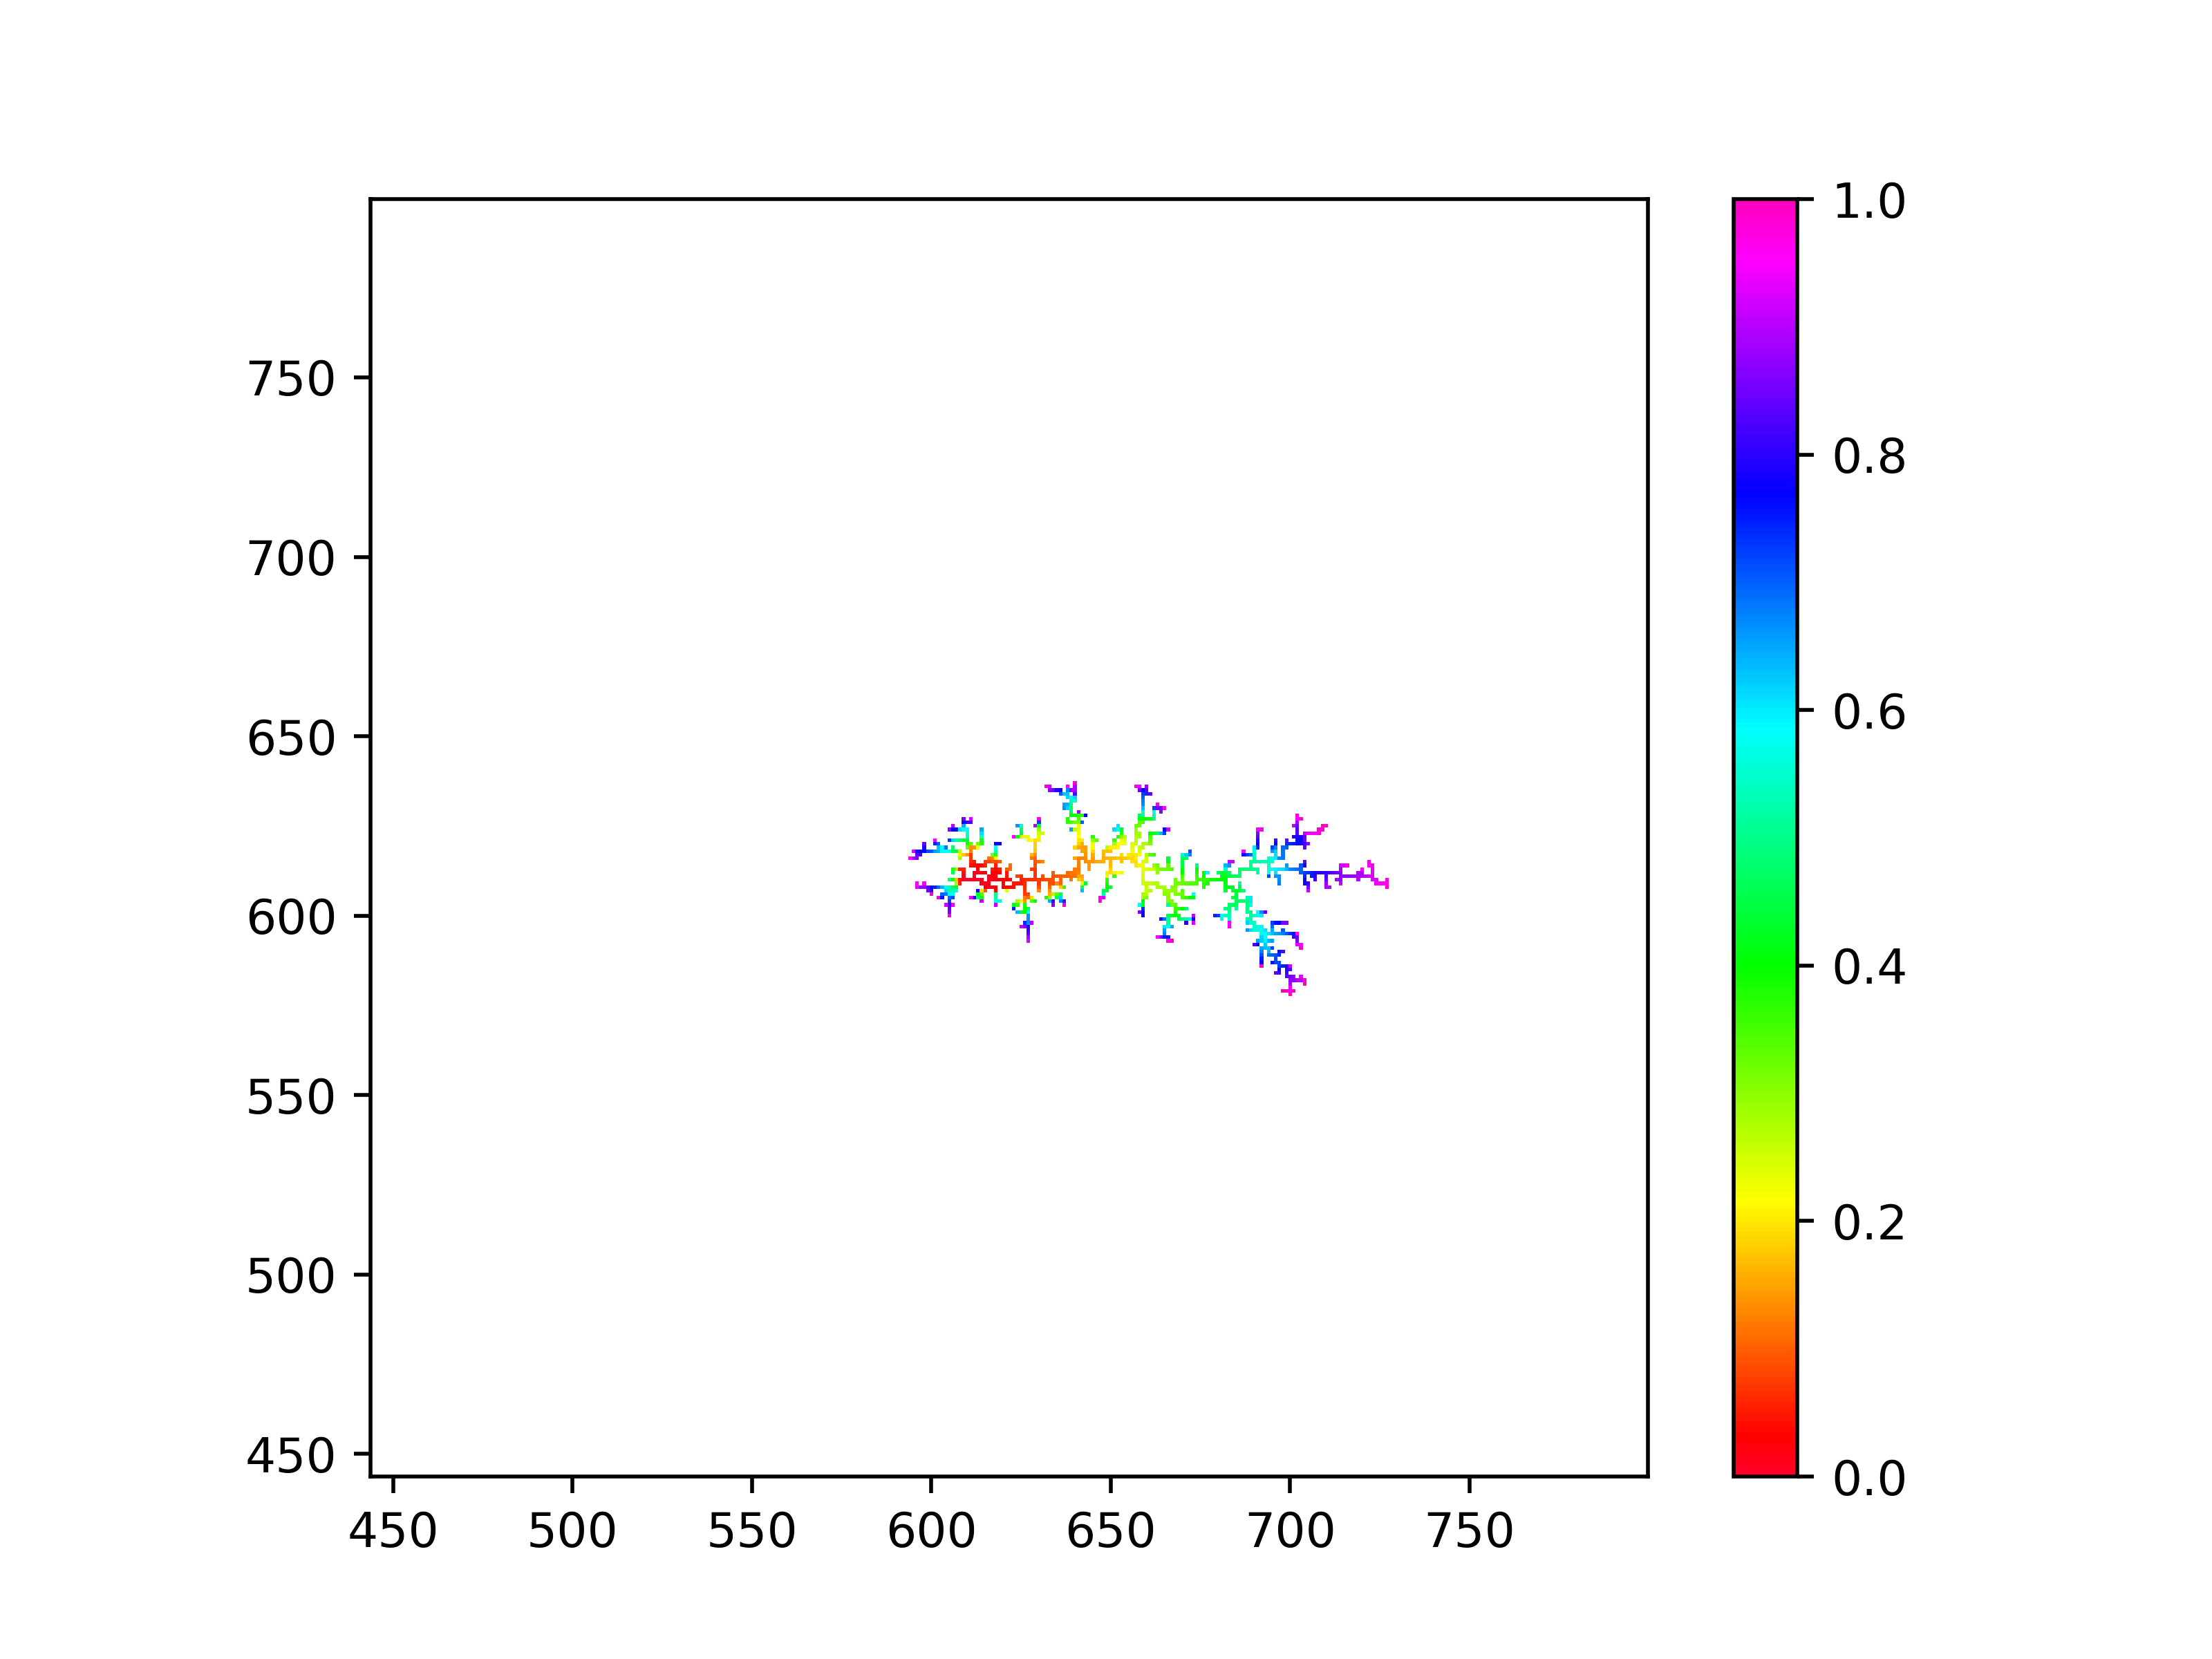
\includegraphics[width=\textwidth]{Figure_10_1.1}
		\caption{C=4.30\% Rmv=1.1}
	\end{subfigure}
	\hfill
	\begin{subfigure}[b]{0.2\textwidth}
		\centering
		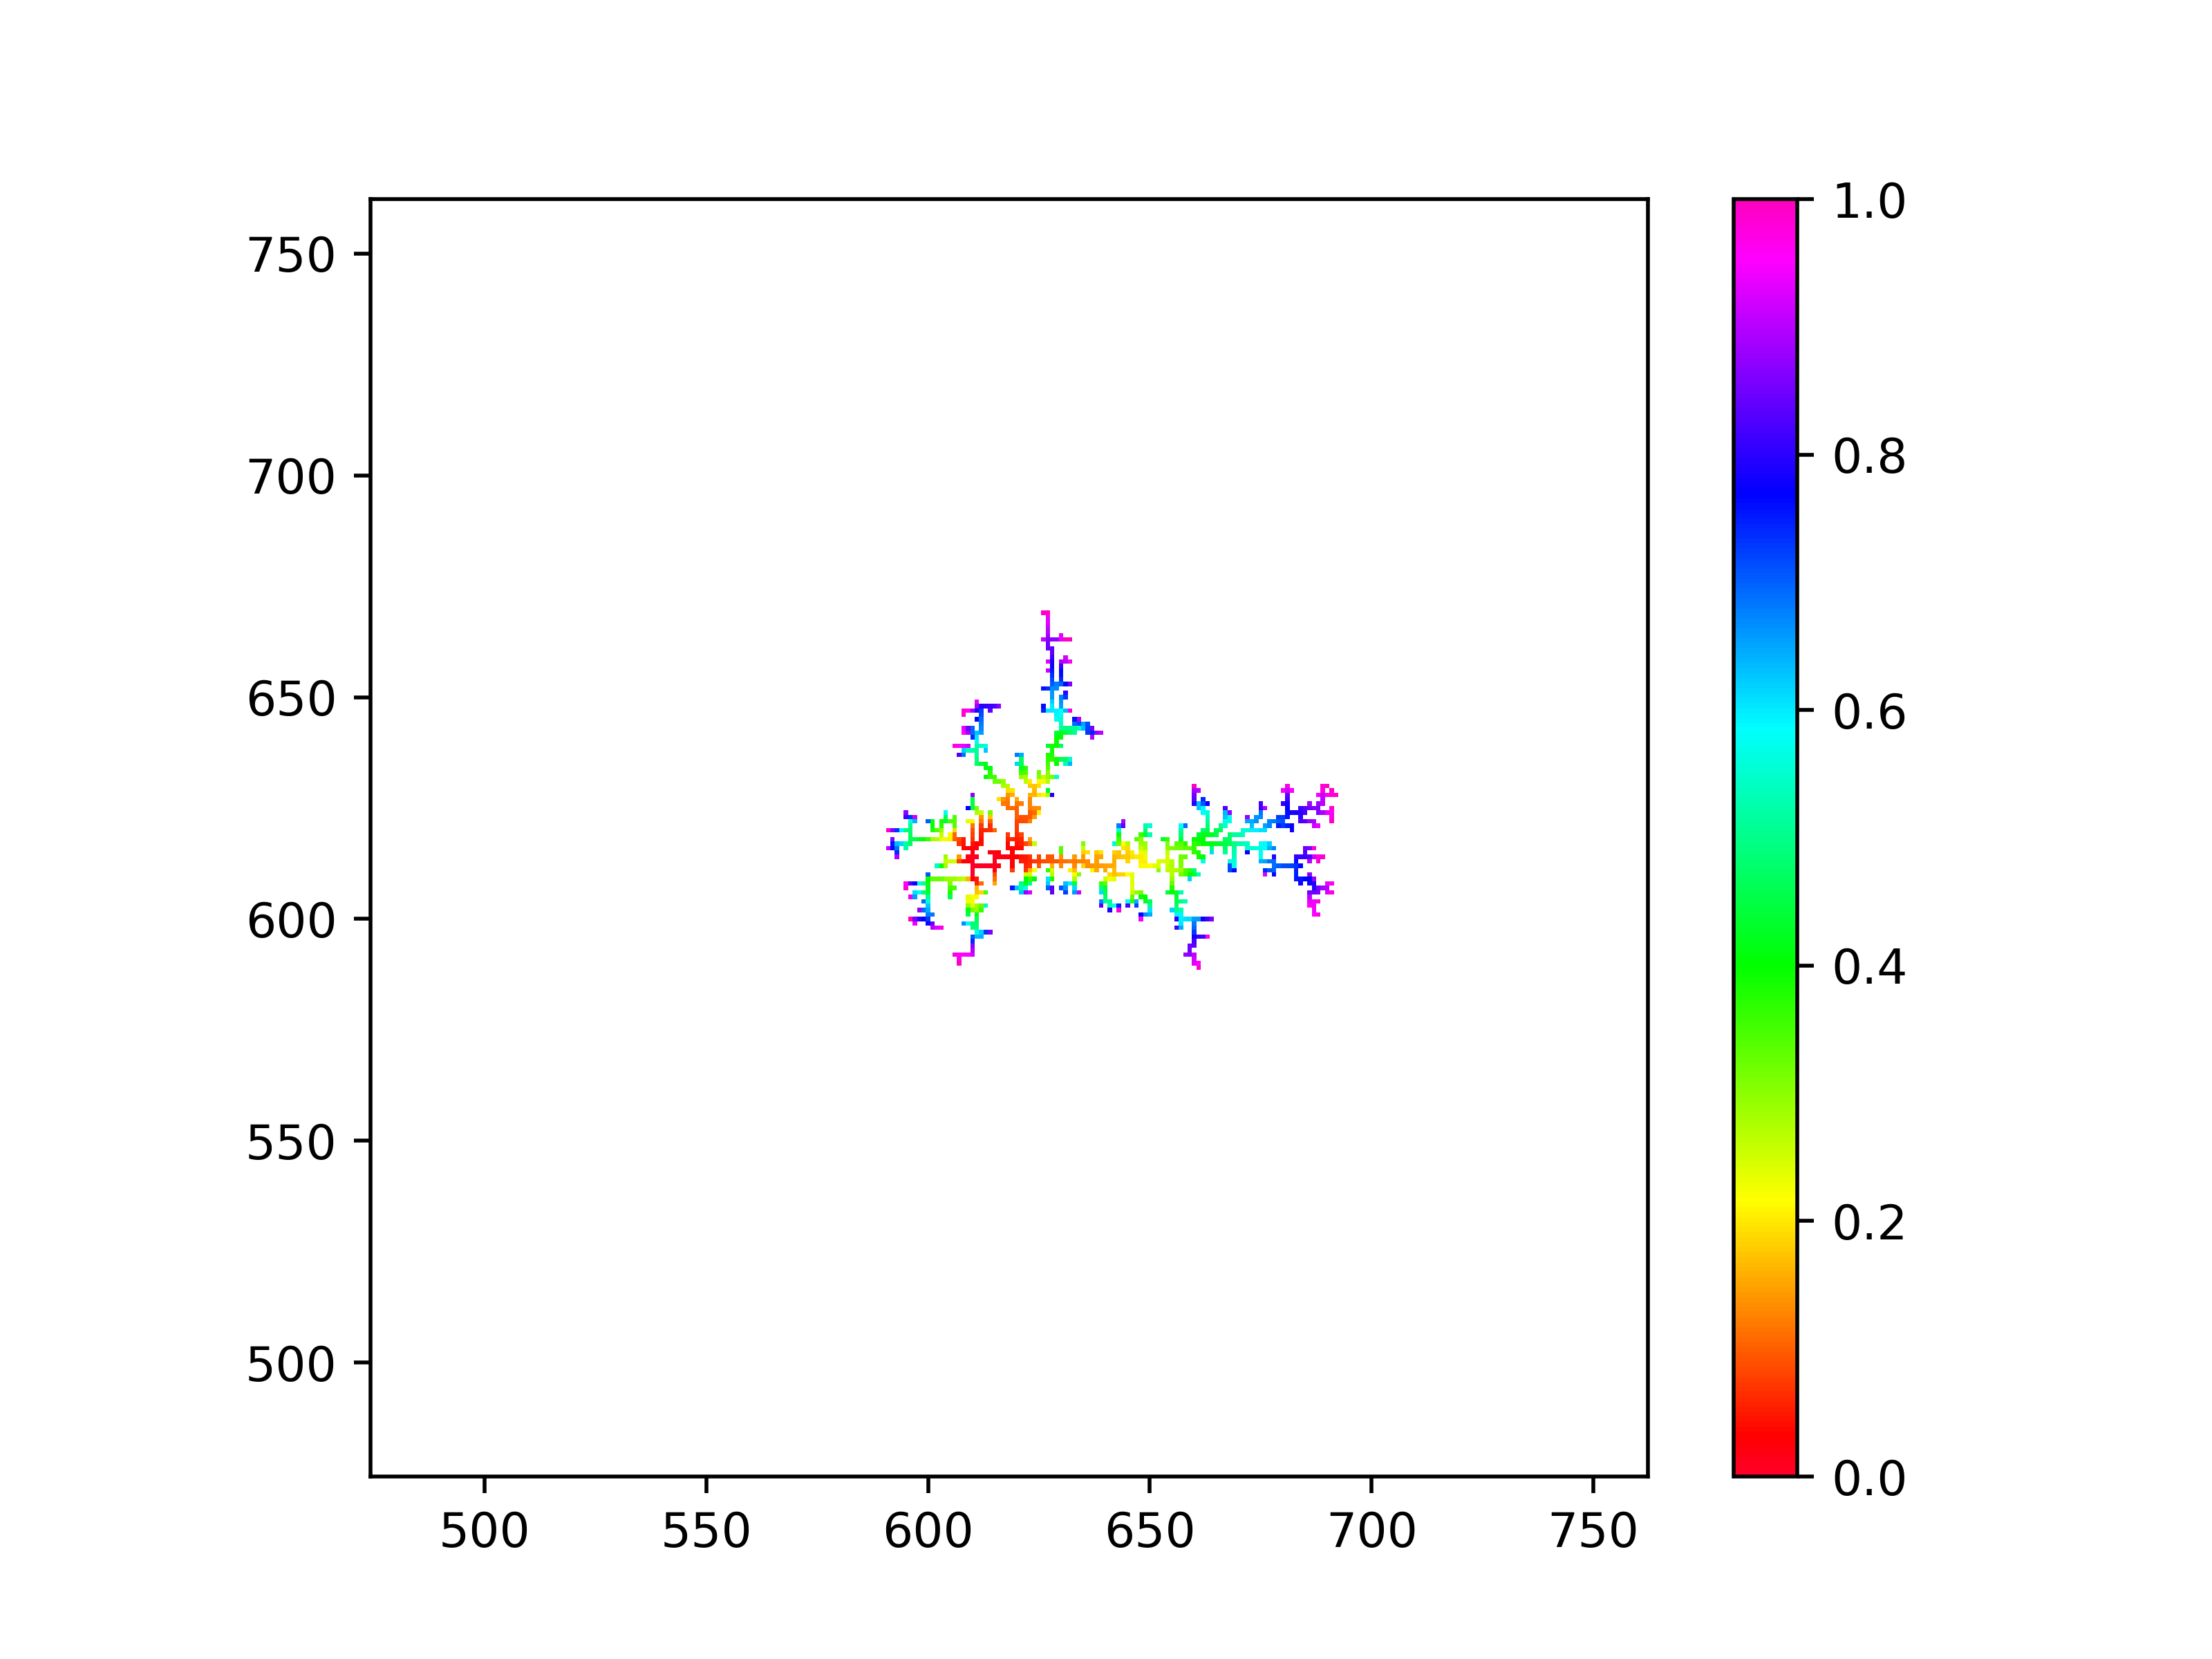
\includegraphics[width=\textwidth]{Figure_10_1.2}
		\caption{C=9.96\% Rmv=1.2}
	\end{subfigure}
	\hfill
	\begin{subfigure}[b]{0.2\textwidth}
		\centering
		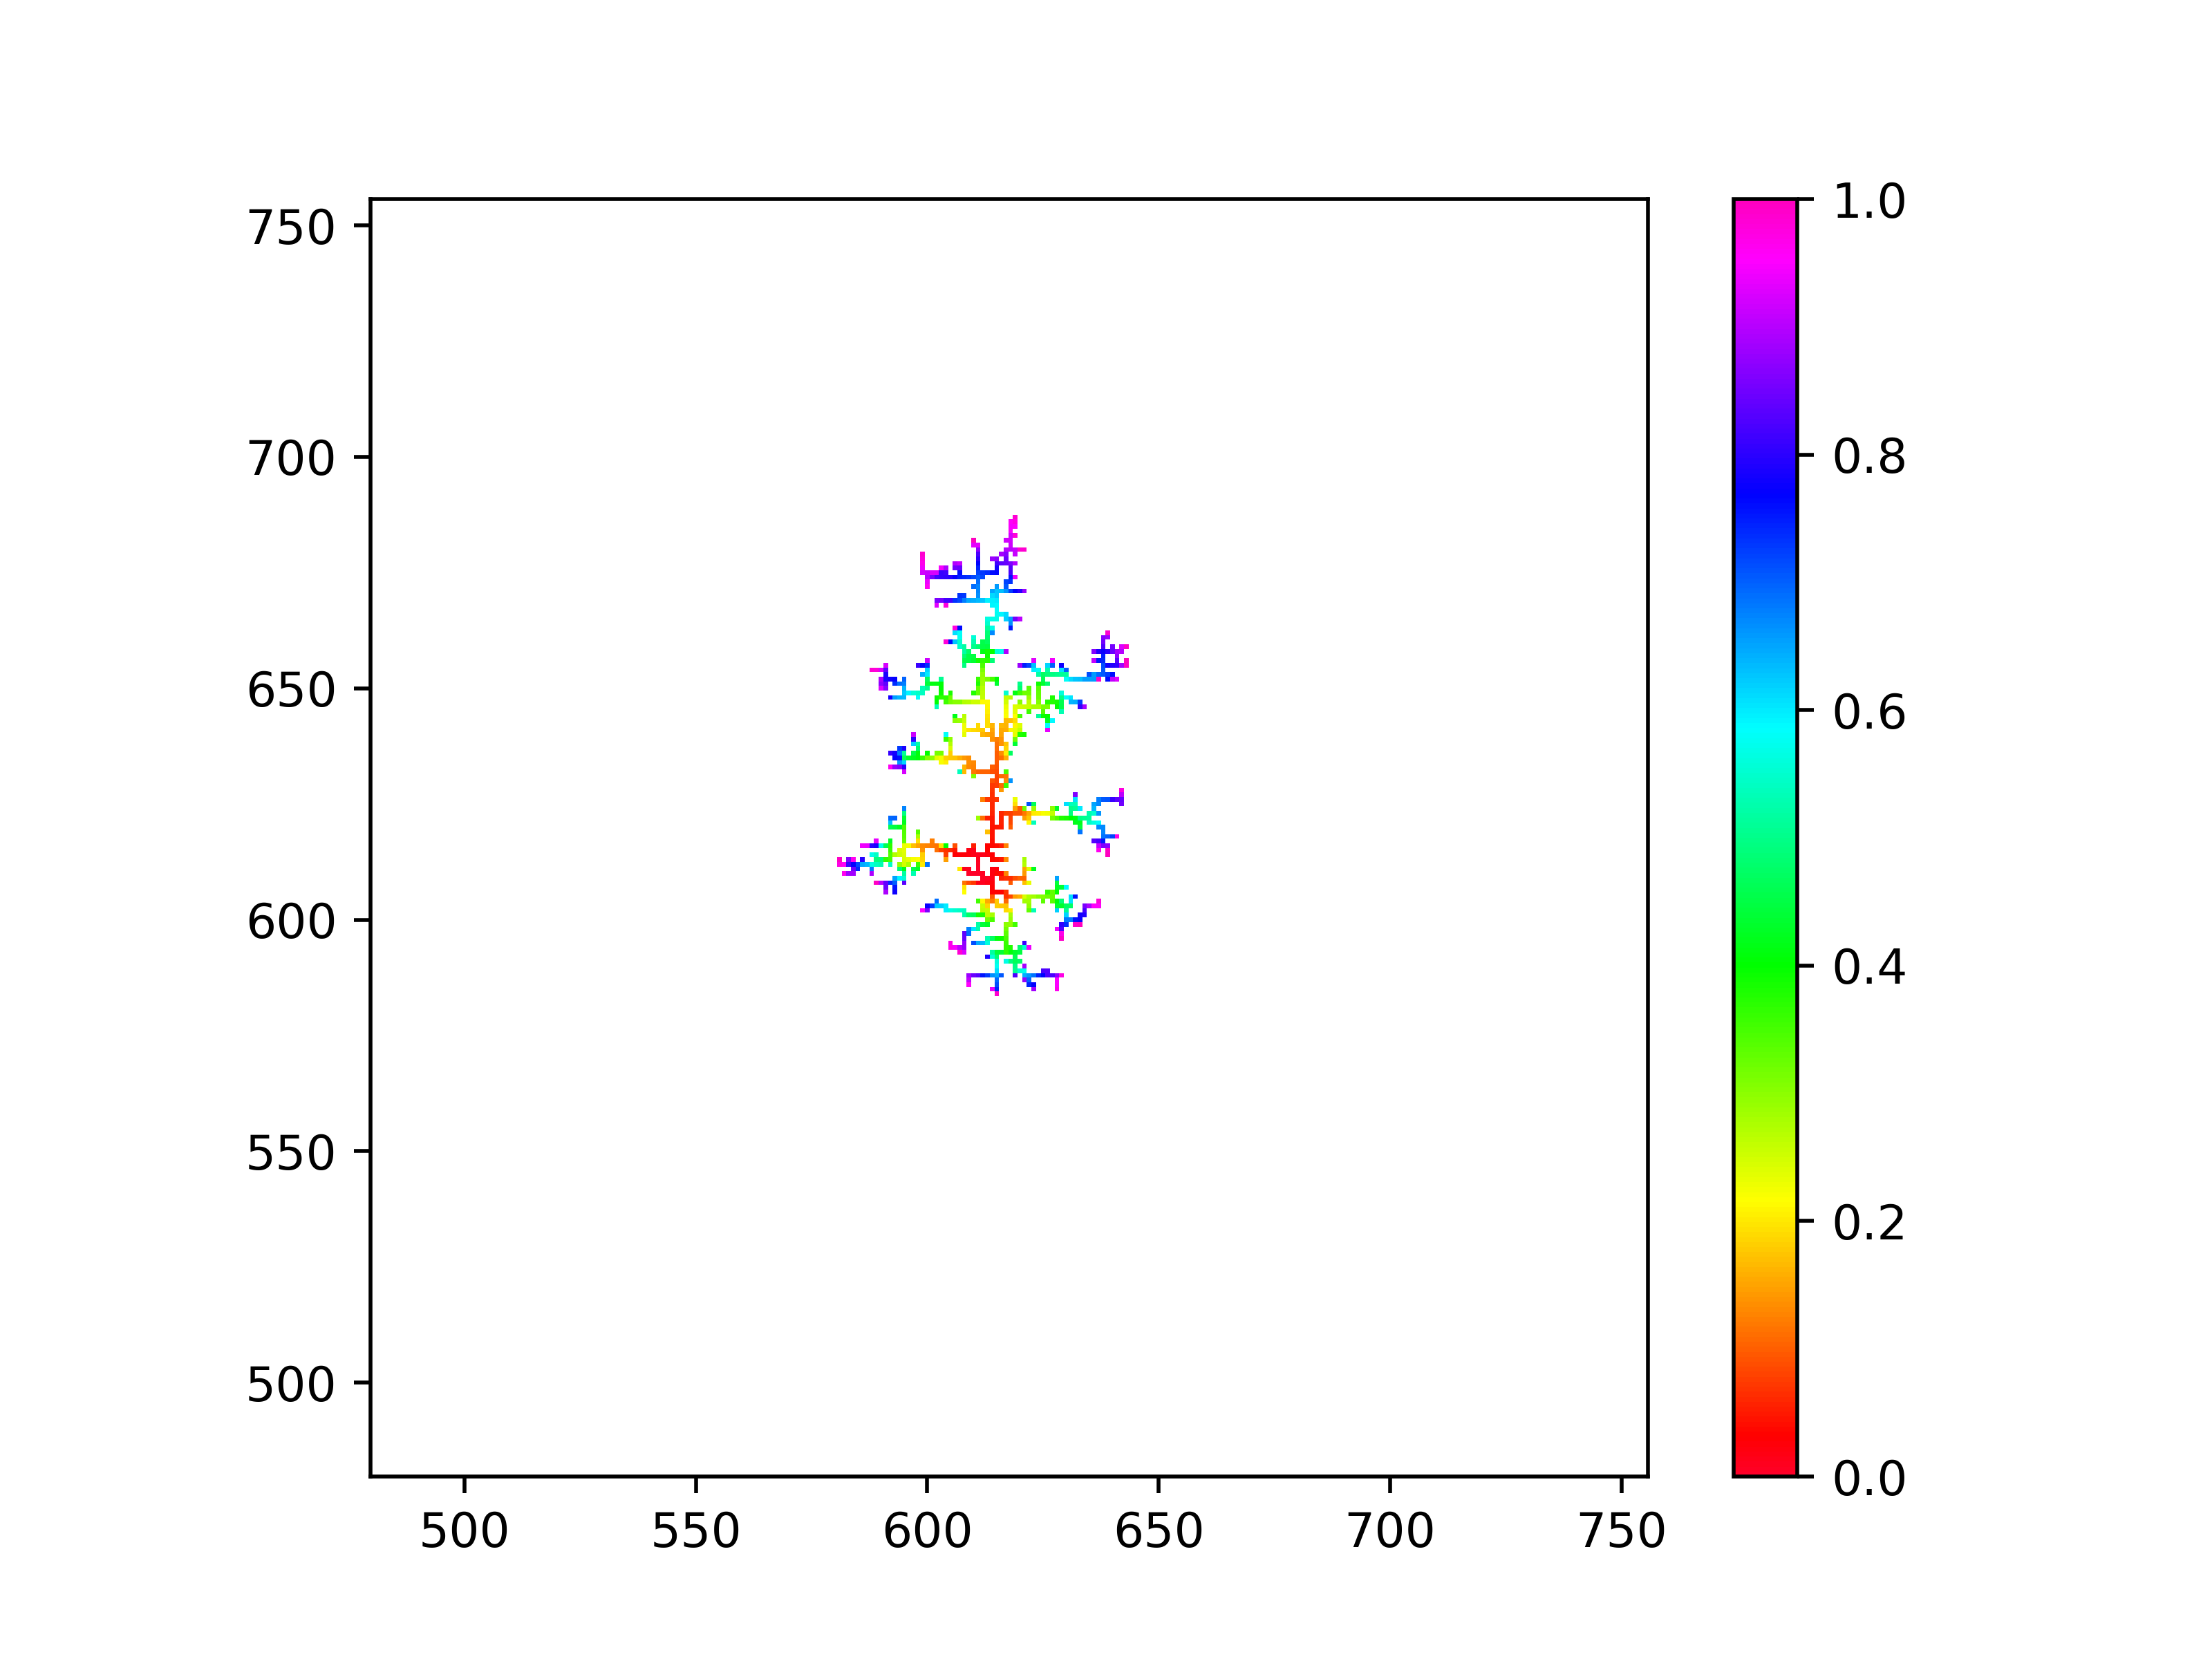
\includegraphics[width=\textwidth]{Figure_10_1.3}
		\caption{C=17.45\% Rmv=1.3}
	\end{subfigure}
	\hfill
	\begin{subfigure}[b]{0.2\textwidth}
		\centering
		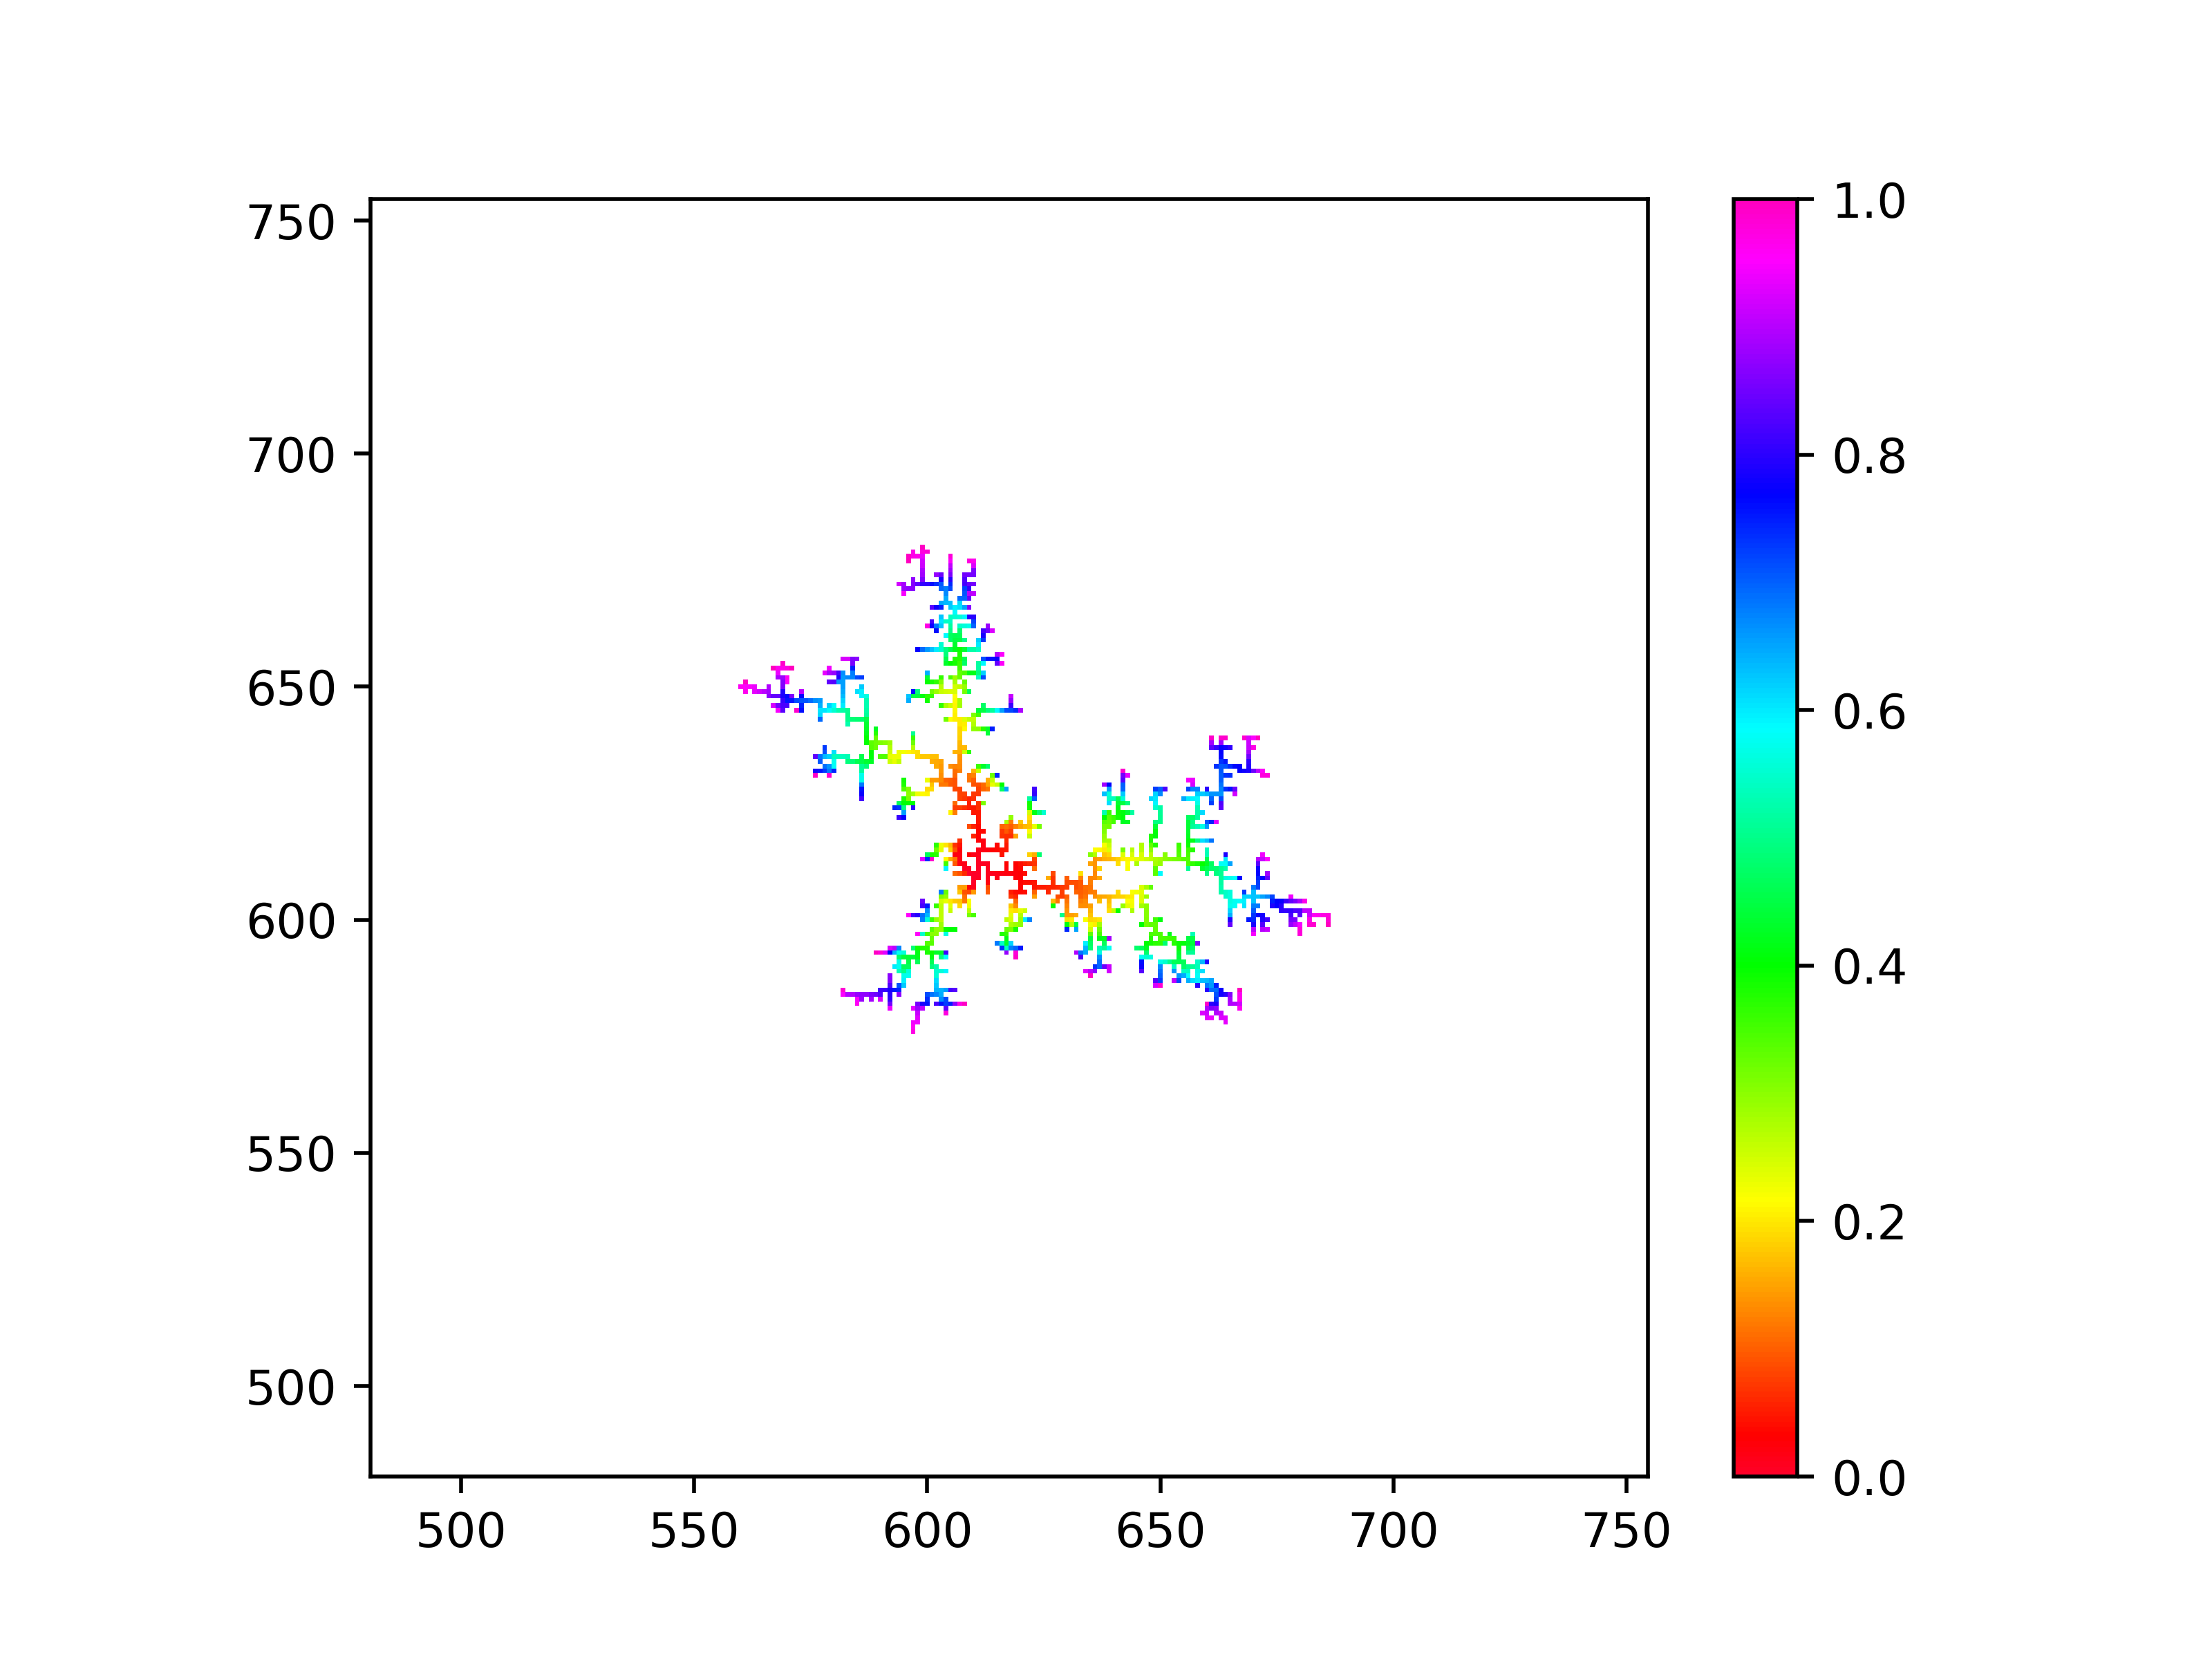
\includegraphics[width=\textwidth]{Figure_10_1.4}
		\caption{C=25.16\% Rmv=1.4}
	\end{subfigure}
	\hfill
	\begin{subfigure}[b]{0.2\textwidth}
		\centering
		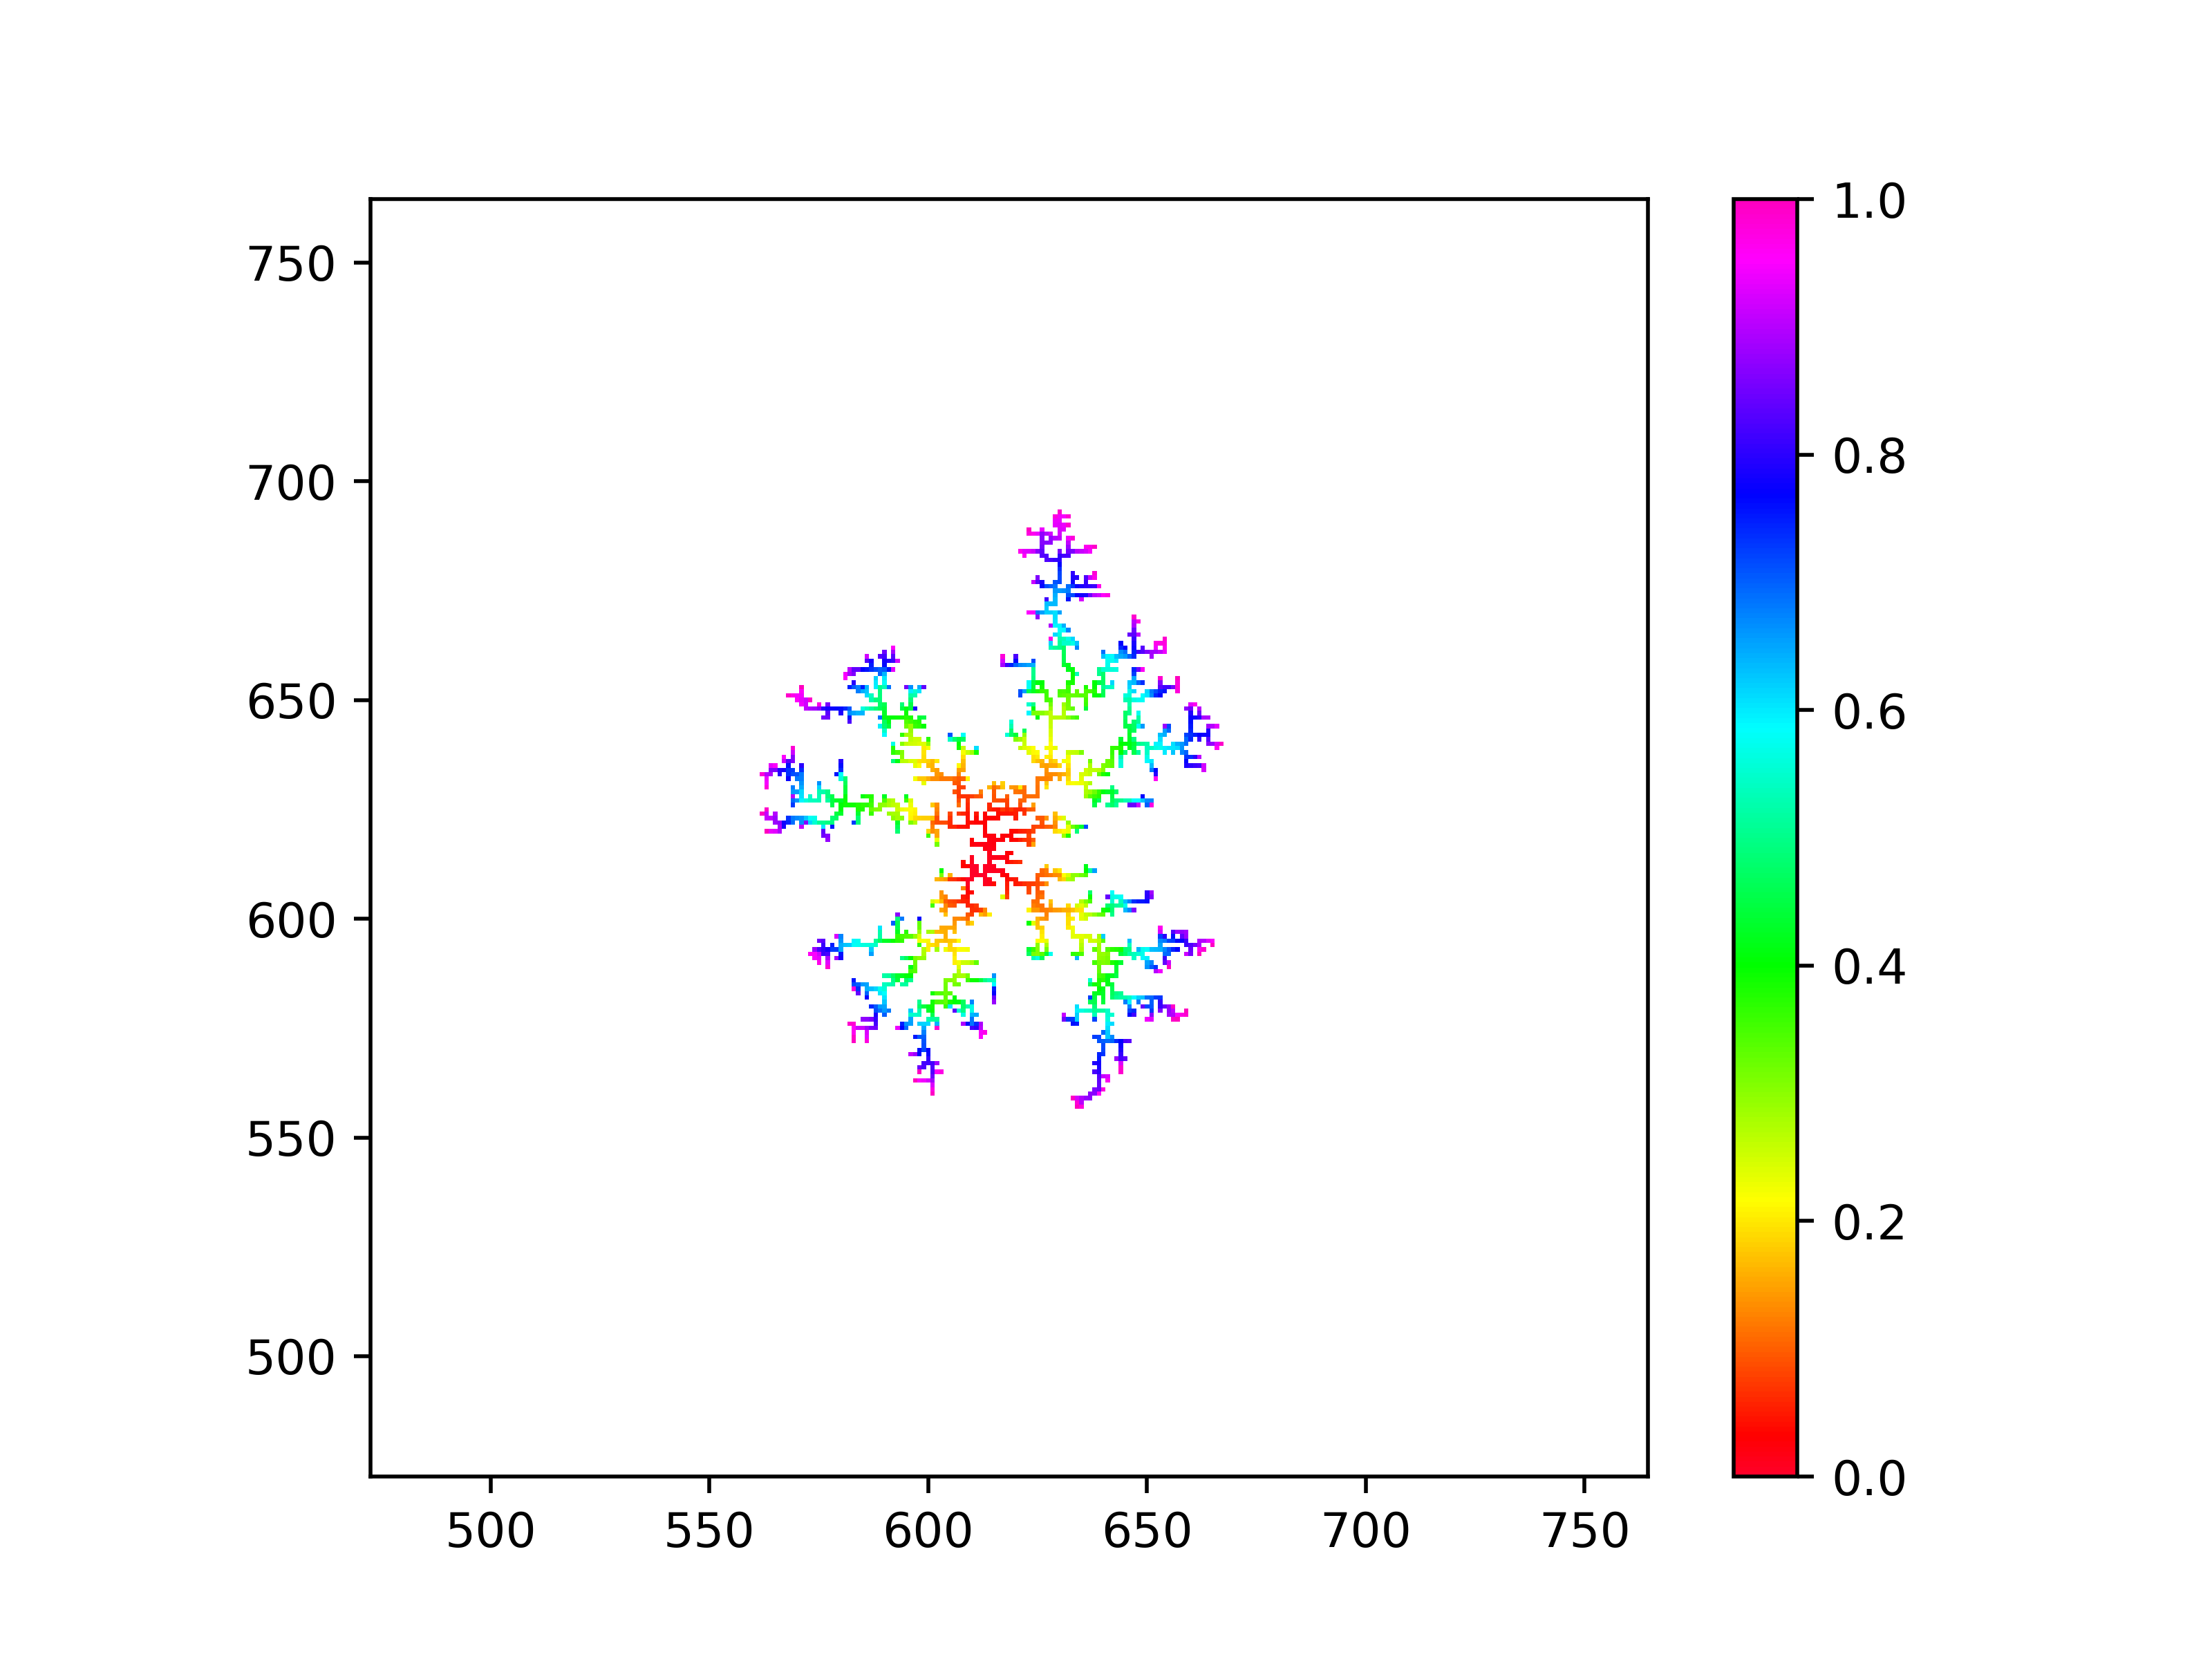
\includegraphics[width=\textwidth]{Figure_10_1.5}
		\caption{C=32.86\% Rmv=1.5}
	\end{subfigure}
	\hfill
	\begin{subfigure}[b]{0.2\textwidth}
		\centering
		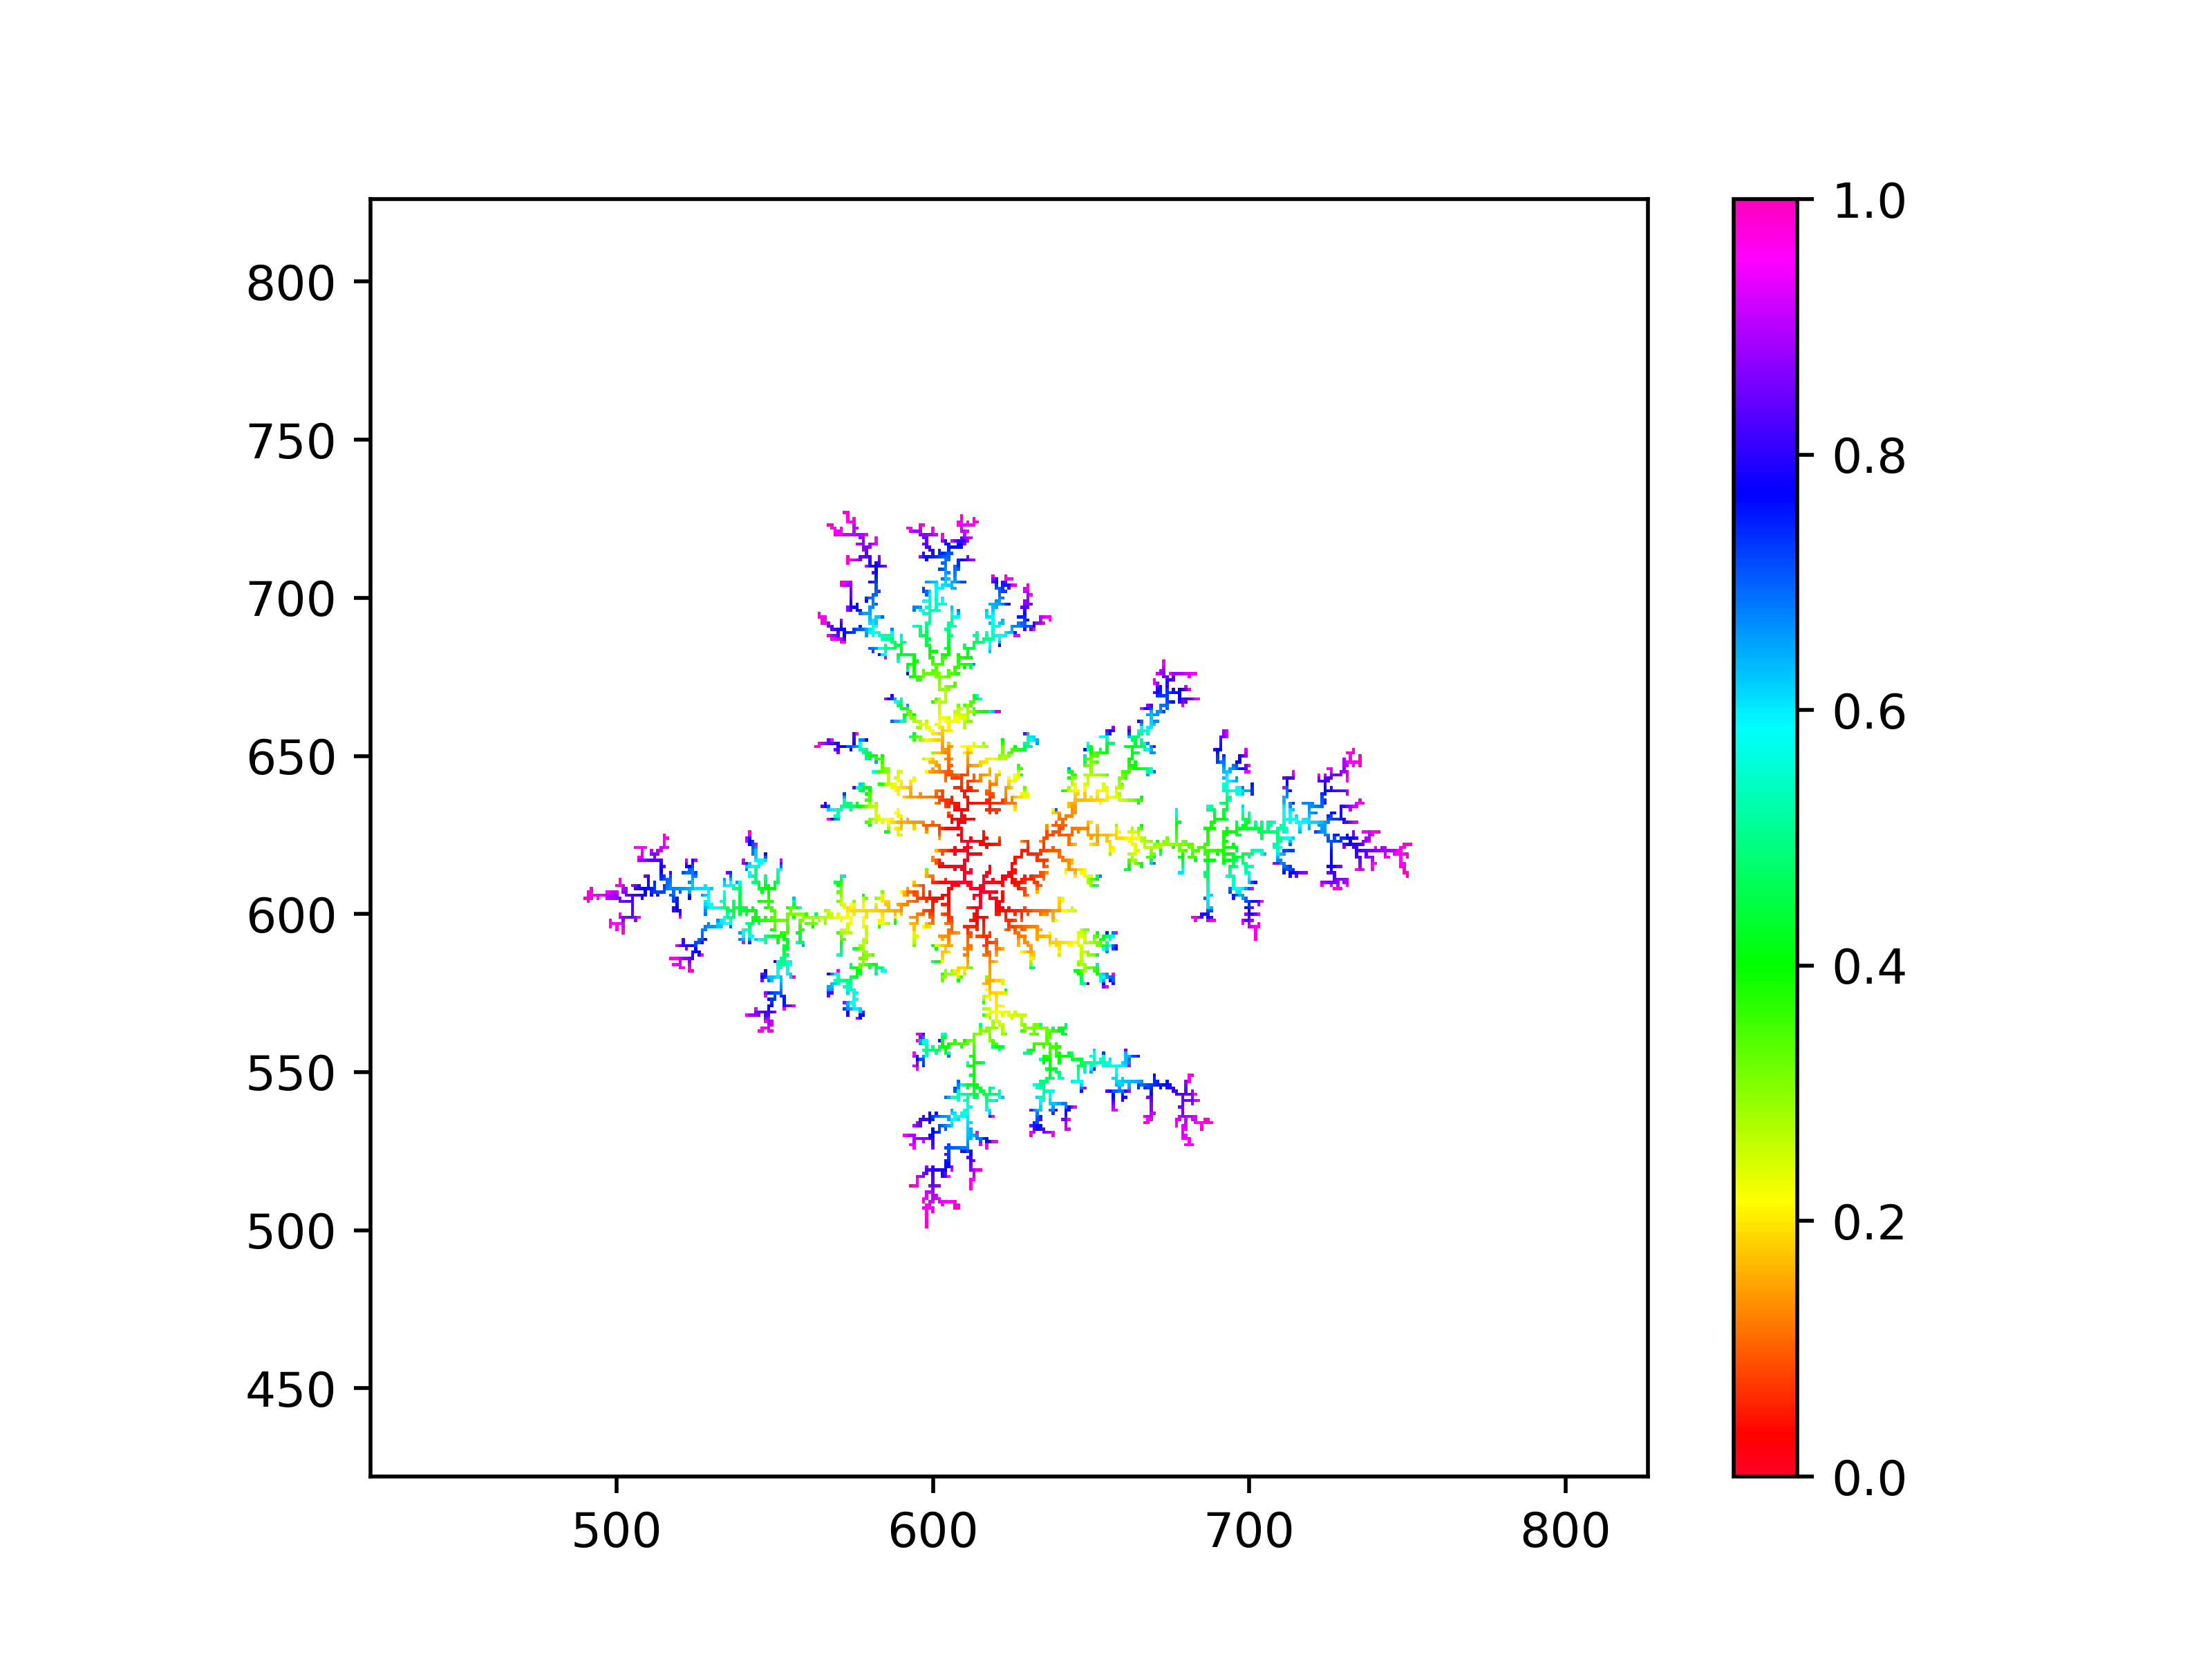
\includegraphics[width=\textwidth]{Figure_10_2}
		\caption{C=56.46\% Rmv=2}
	\end{subfigure}
	\hfill
	\begin{subfigure}[b]{0.2\textwidth}
		\centering
		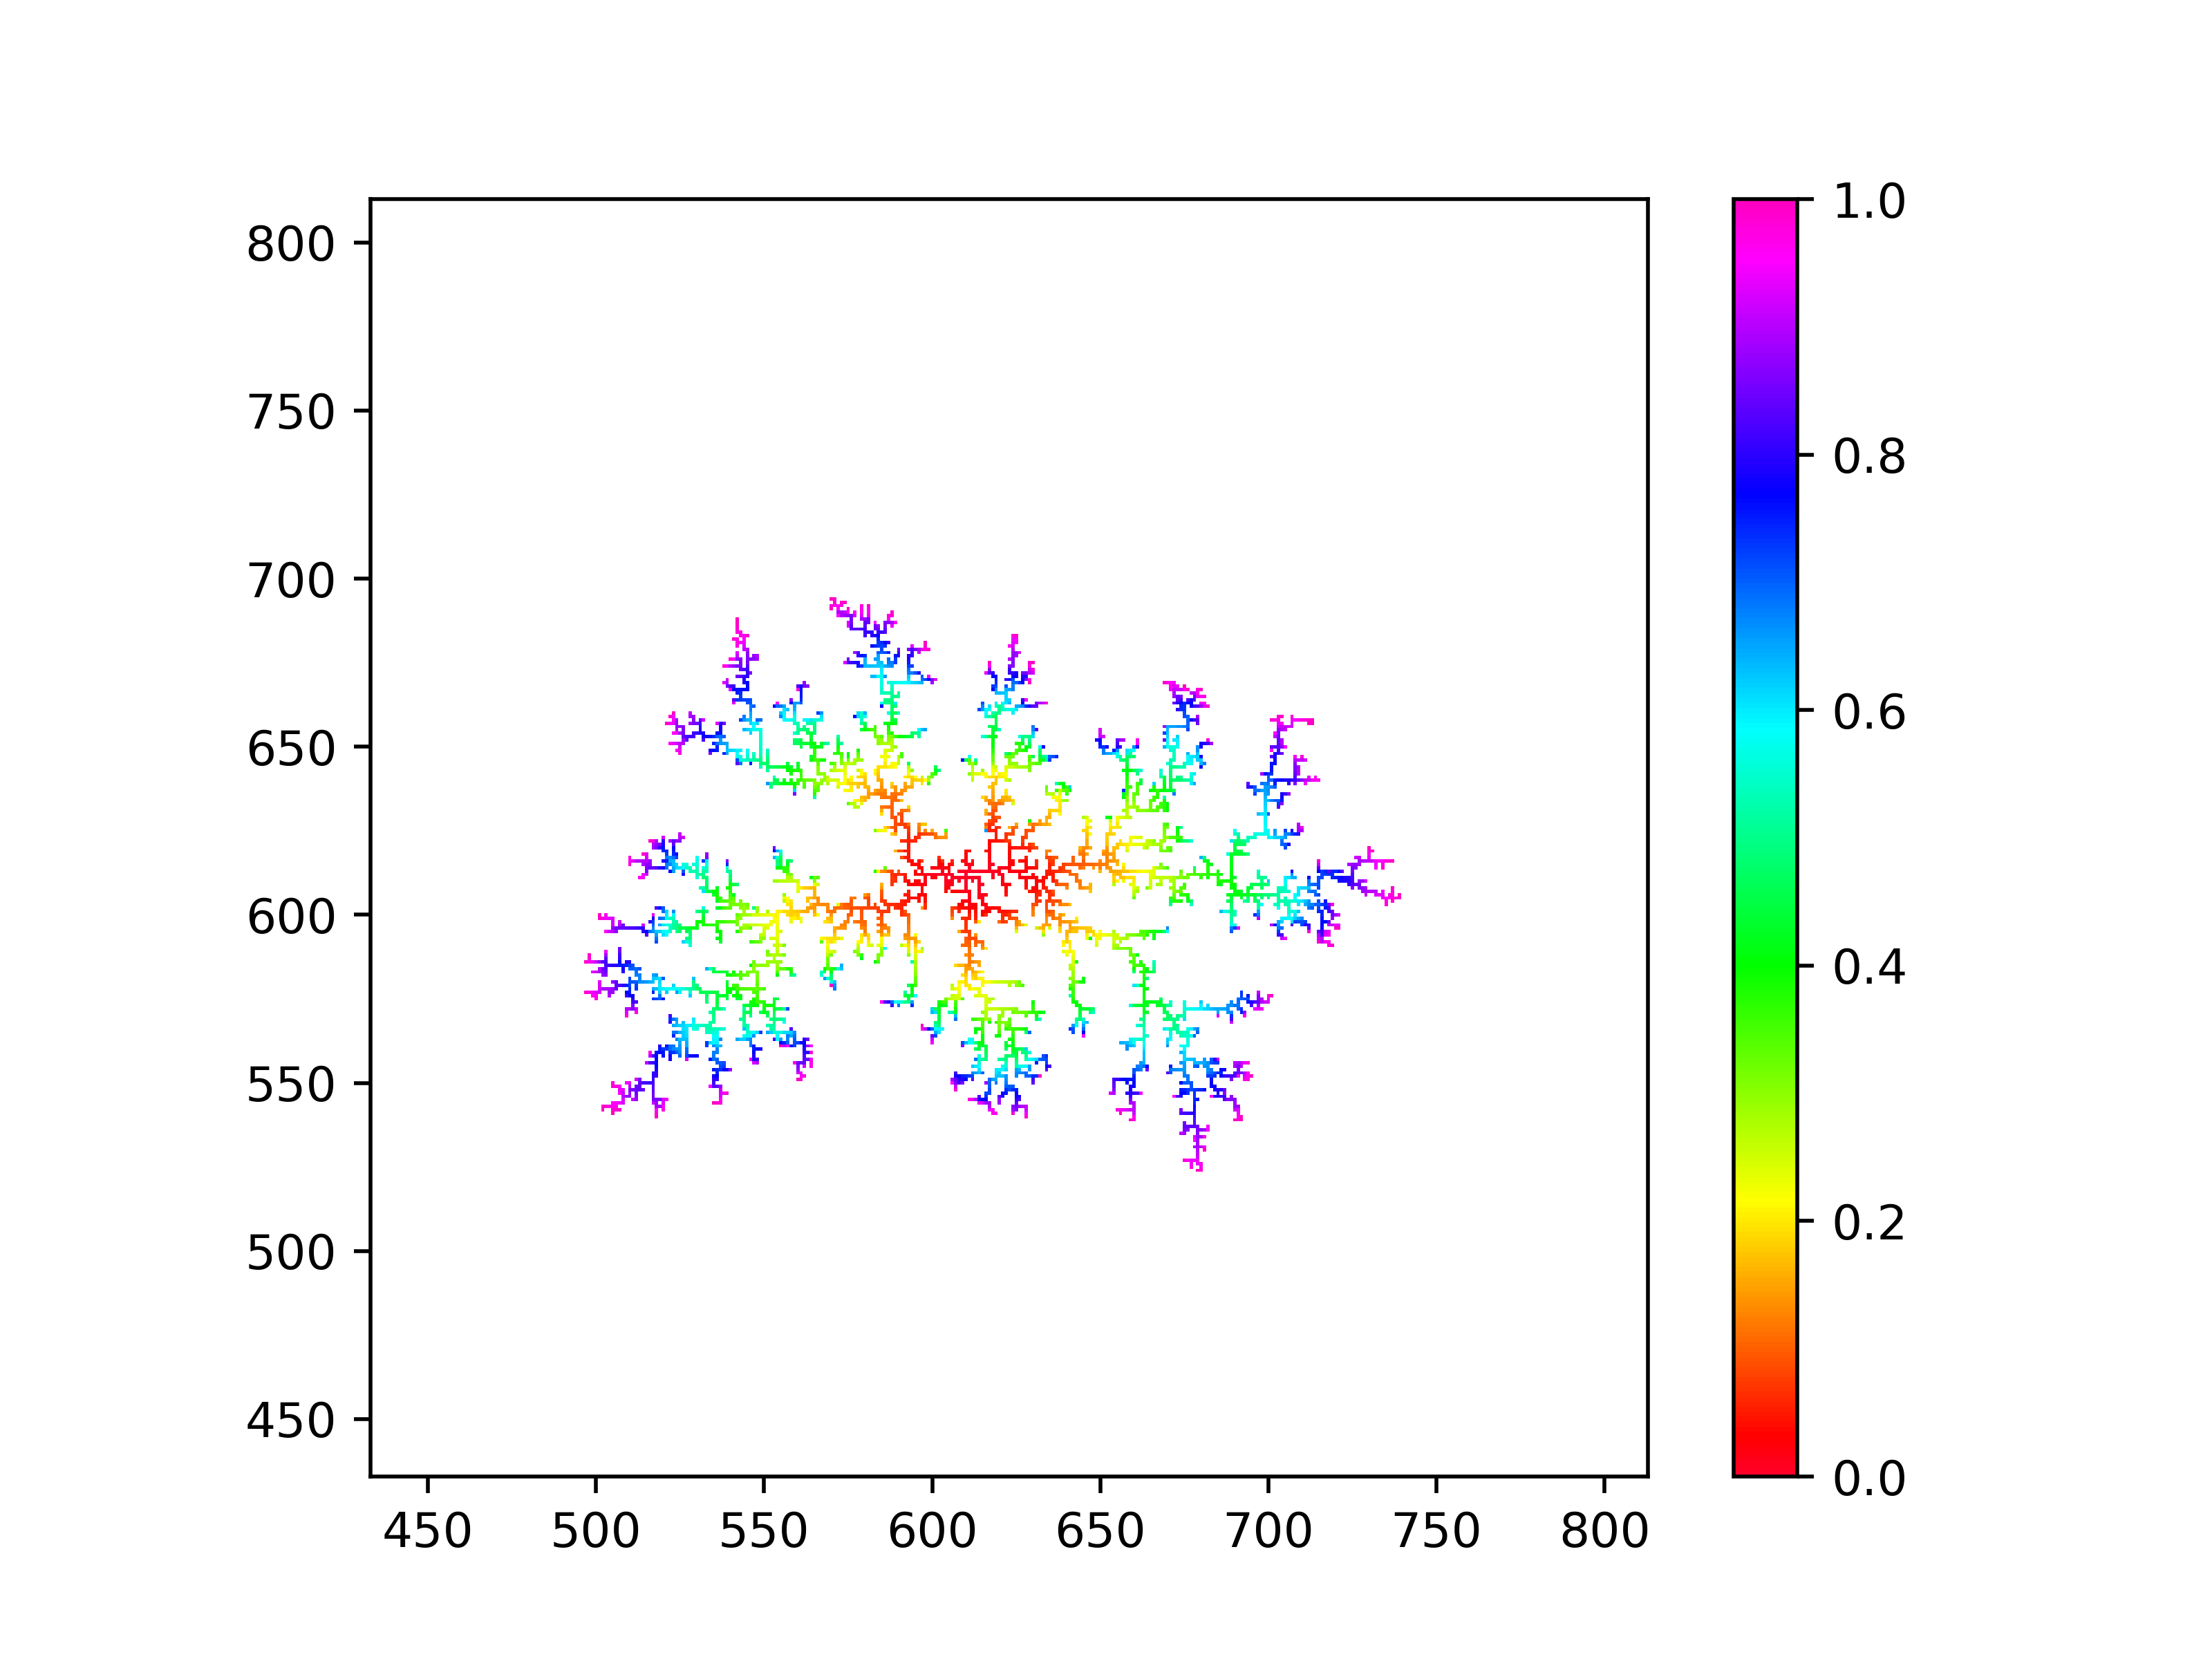
\includegraphics[width=\textwidth]{Figure_10_3}
		\caption{C=71.71\% Rmv=3}
	\end{subfigure}
	\caption{Clusterings of Different Removing Ranges}
\end{figure}

In Figure 6 above, the variable C refers to the clustering rate defined as before, Rmv refers to the ratio between R\_remove and current maximum radius.

We can see intuitively that the clustering rate rises dramatically as the ratio increases, which obeys our intuition. What we actually concern is that, when the ratio is small enough, the clustering result shows a remarkable directionality, which we are going to discuss next.

We build our model shown in Figure 7 below. Suppose the current cluster is shown as the red branches, the current input radius is of the same multiple as the current maximum clustering radius, while the remove range is of several multiple compare to the current maximum clustering radius.

\begin{center}
	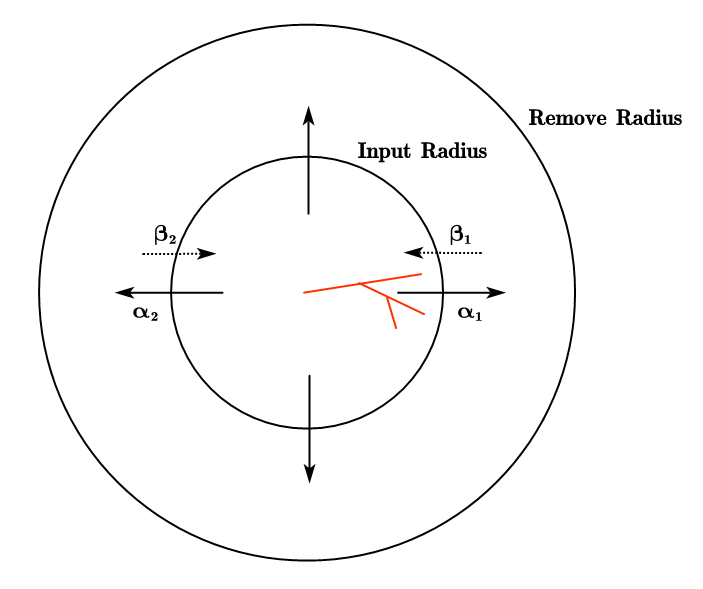
\includegraphics[width=0.4\textwidth]{Figure_11}
	\captionof{figure}{Model of the Impact of Removing Range}
\end{center}

Suppose at the current time, the cluster perform its directionality to the right side. We define $\alpha_{1,2}$ \& $\beta_{1,2}$ shown in the figure above, which represents the percentage of the input particle that travel through the "membrane" just at the radius of the input radius. For simplicity, we assume that the particles only pass the "membrane" at the two side, shown in the figure. Thus, we use $\alpha_{1,2}$ \& $\beta_{1,2}$ to represent all the particles that pass through the "membrane".

It's easy to obtain that $\alpha_{1} < \alpha_{2}$, since it's more likely to cluster, according to the figure. We first consider the extreme case, where the remove radius is of the same order as the input radius. This can be viewed as a reallocation of the particle as soon as it goes out of the remove radius. When it's small enough, the two parameters $\alpha_{1}$ and $\alpha_{2}$ have a great difference ($\alpha_{2} >> \alpha_{1}$), but since the re-input of the particle is random on the circle, the two parameters $\beta_{1}$ and $\beta_{2}$ are almost the same by the "reallocation" by the mechanism. The difference between the $\alpha_{2}$ and $\alpha_{1}$ has almost been totally erased, results in the fast growth in the direction of the current growth. When the remove radius is large enough, the outgoing particle will also be reallocated, but the ingoing ratios $\beta_{1}$ and $\beta_{2}$ still has a difference, since it's still very difficult for a particle to go from one side of the circle to the other side.

\subsection{2-Dimensional with Distant Sticking}

In this section, we'll enable the distant sticking. For simplicity, we consider the two cases where the adjacent sticking probability being 1 and 0.3, respectively, with the probability to stick with the second nearest neighbor sites being $P_{snn} = \frac{1}{2} P_{nn}$. The two sample clusterings with $P_{nn} = 1$ and $0.3$ out of all the twenty simulations are shown in Figure 8 below. All the twenty results are stored inside the folder \texttt{Second\_Stick}.

\begin{figure}[h]
	\centering
	\begin{subfigure}[b]{0.3\textwidth}
		\centering
		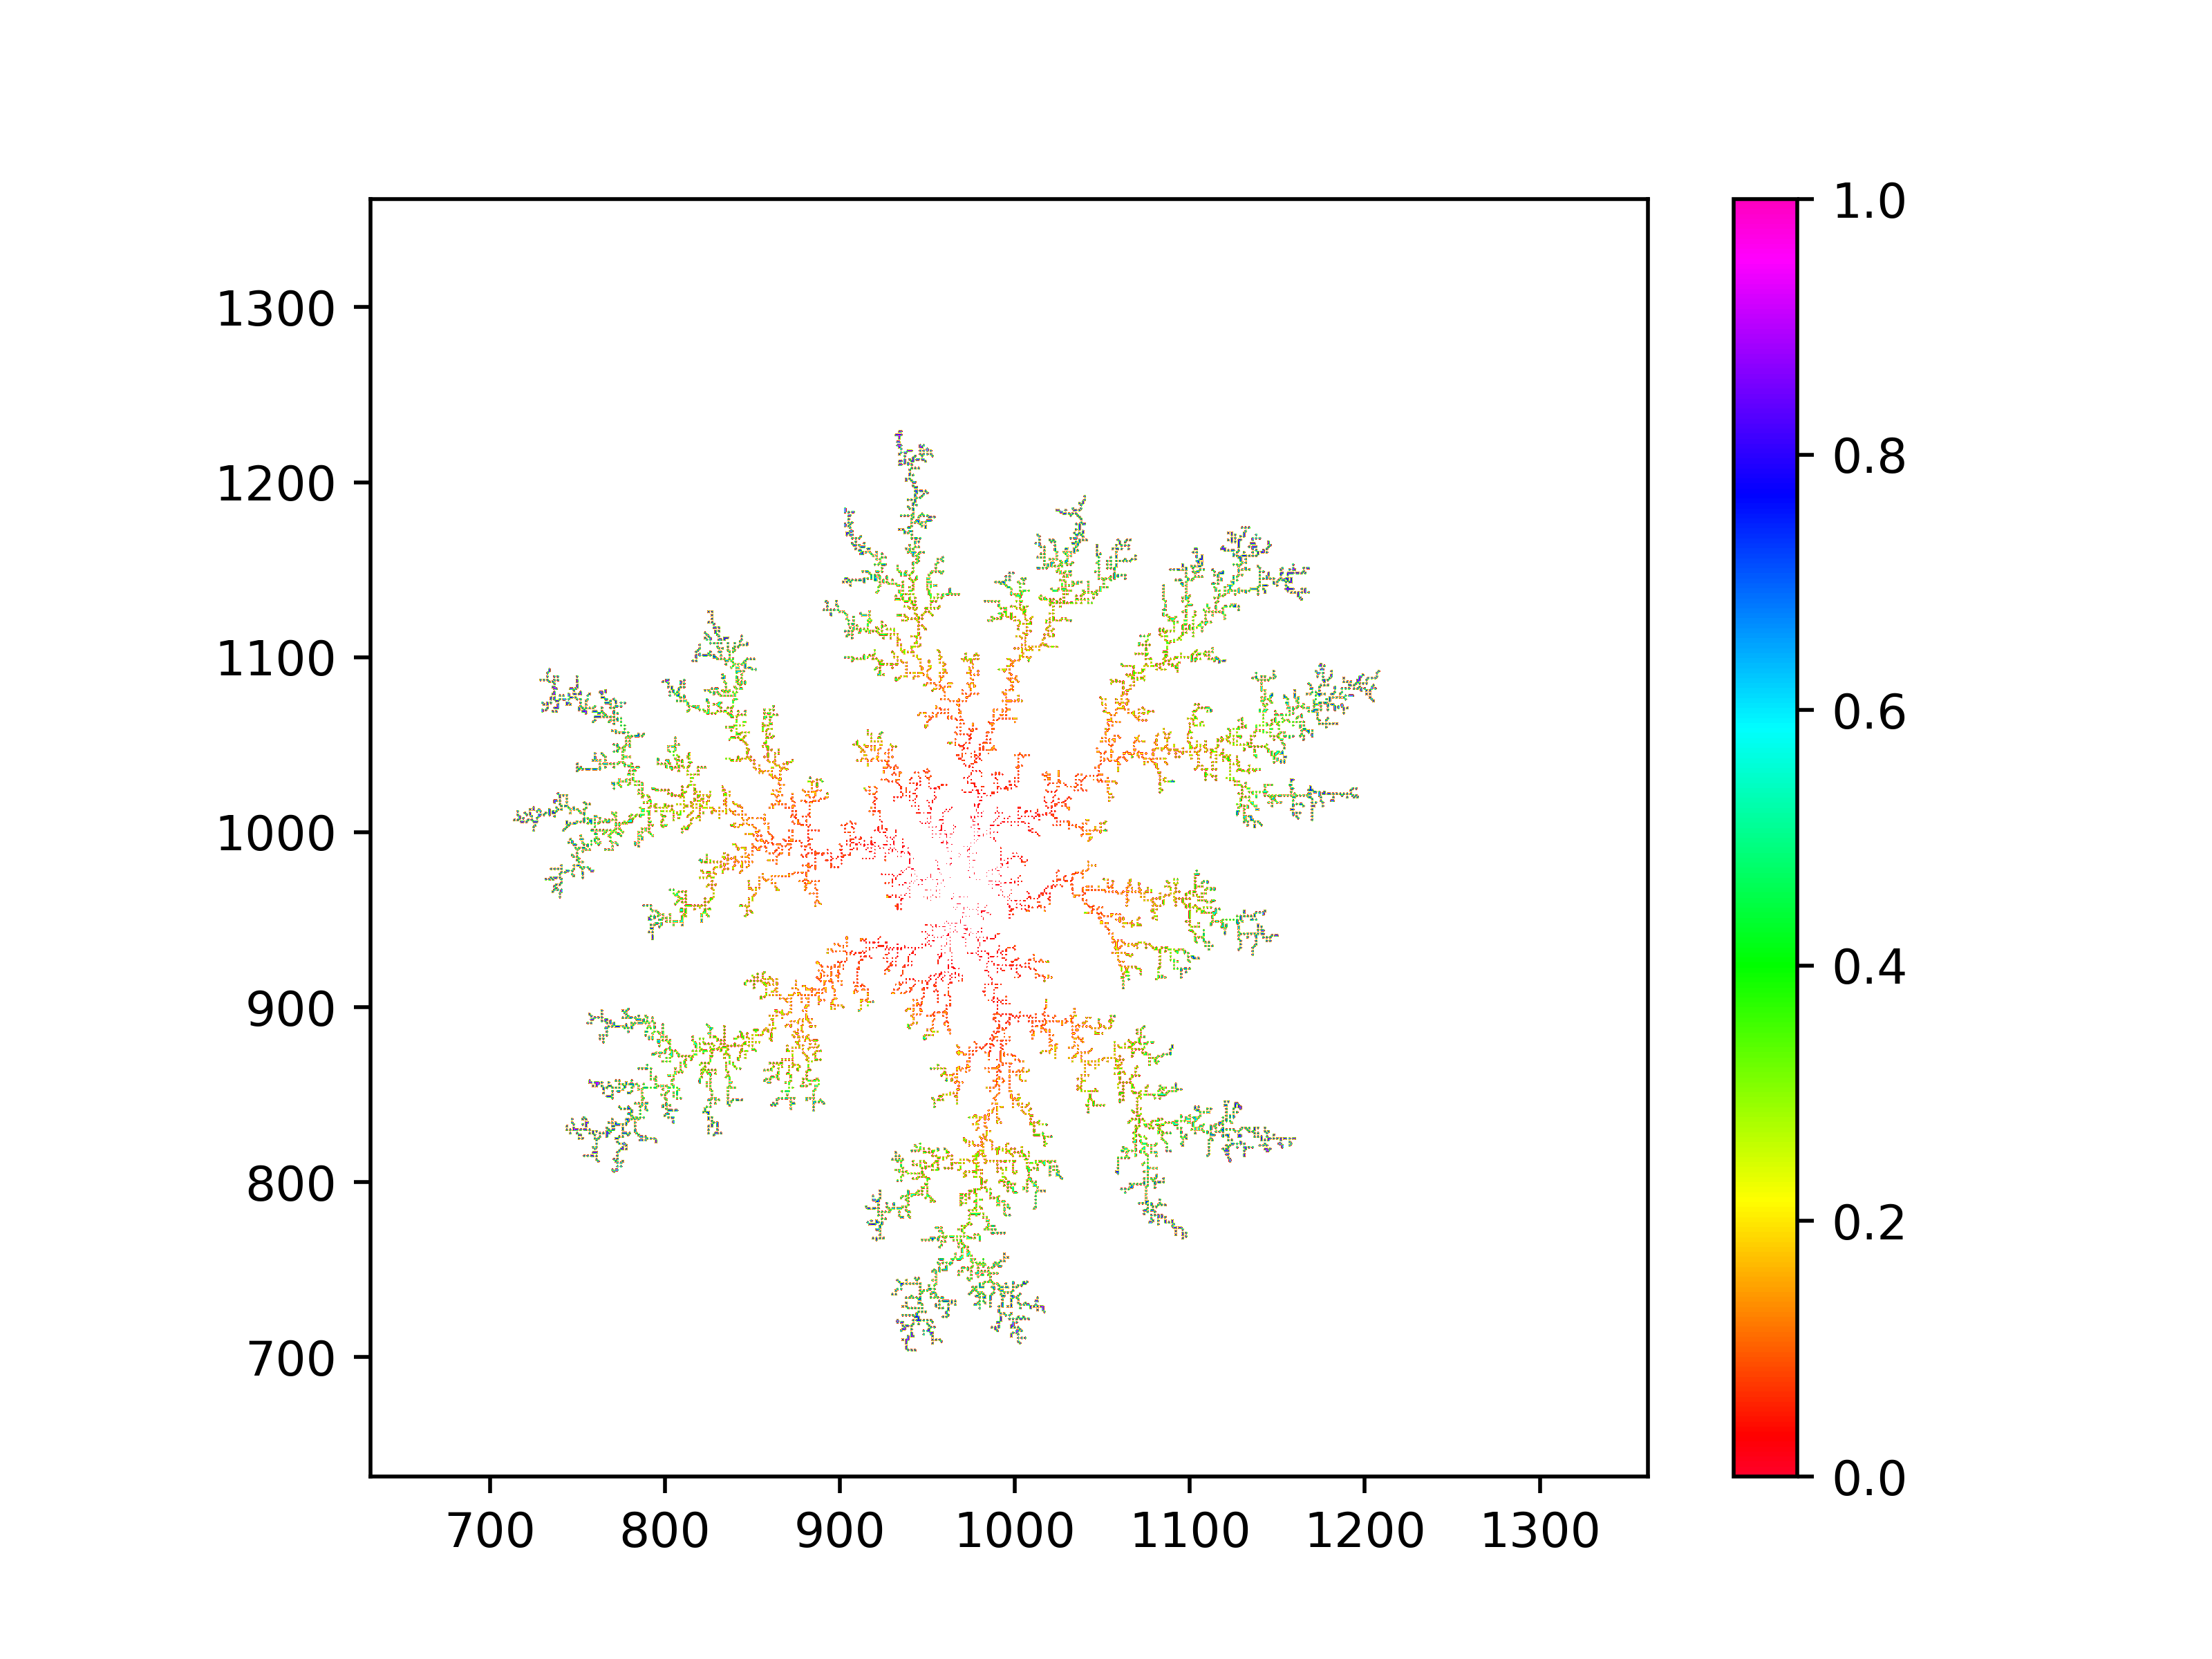
\includegraphics[width=\textwidth]{Figure_12}
		\caption{Adjacent Sticking \#Prob.=100\%, Second Sticking \#Prob.=50\%, clustering rate=82.72\%}
	\end{subfigure}
	% \hfill
	\begin{subfigure}[b]{0.3\textwidth}
		\centering
		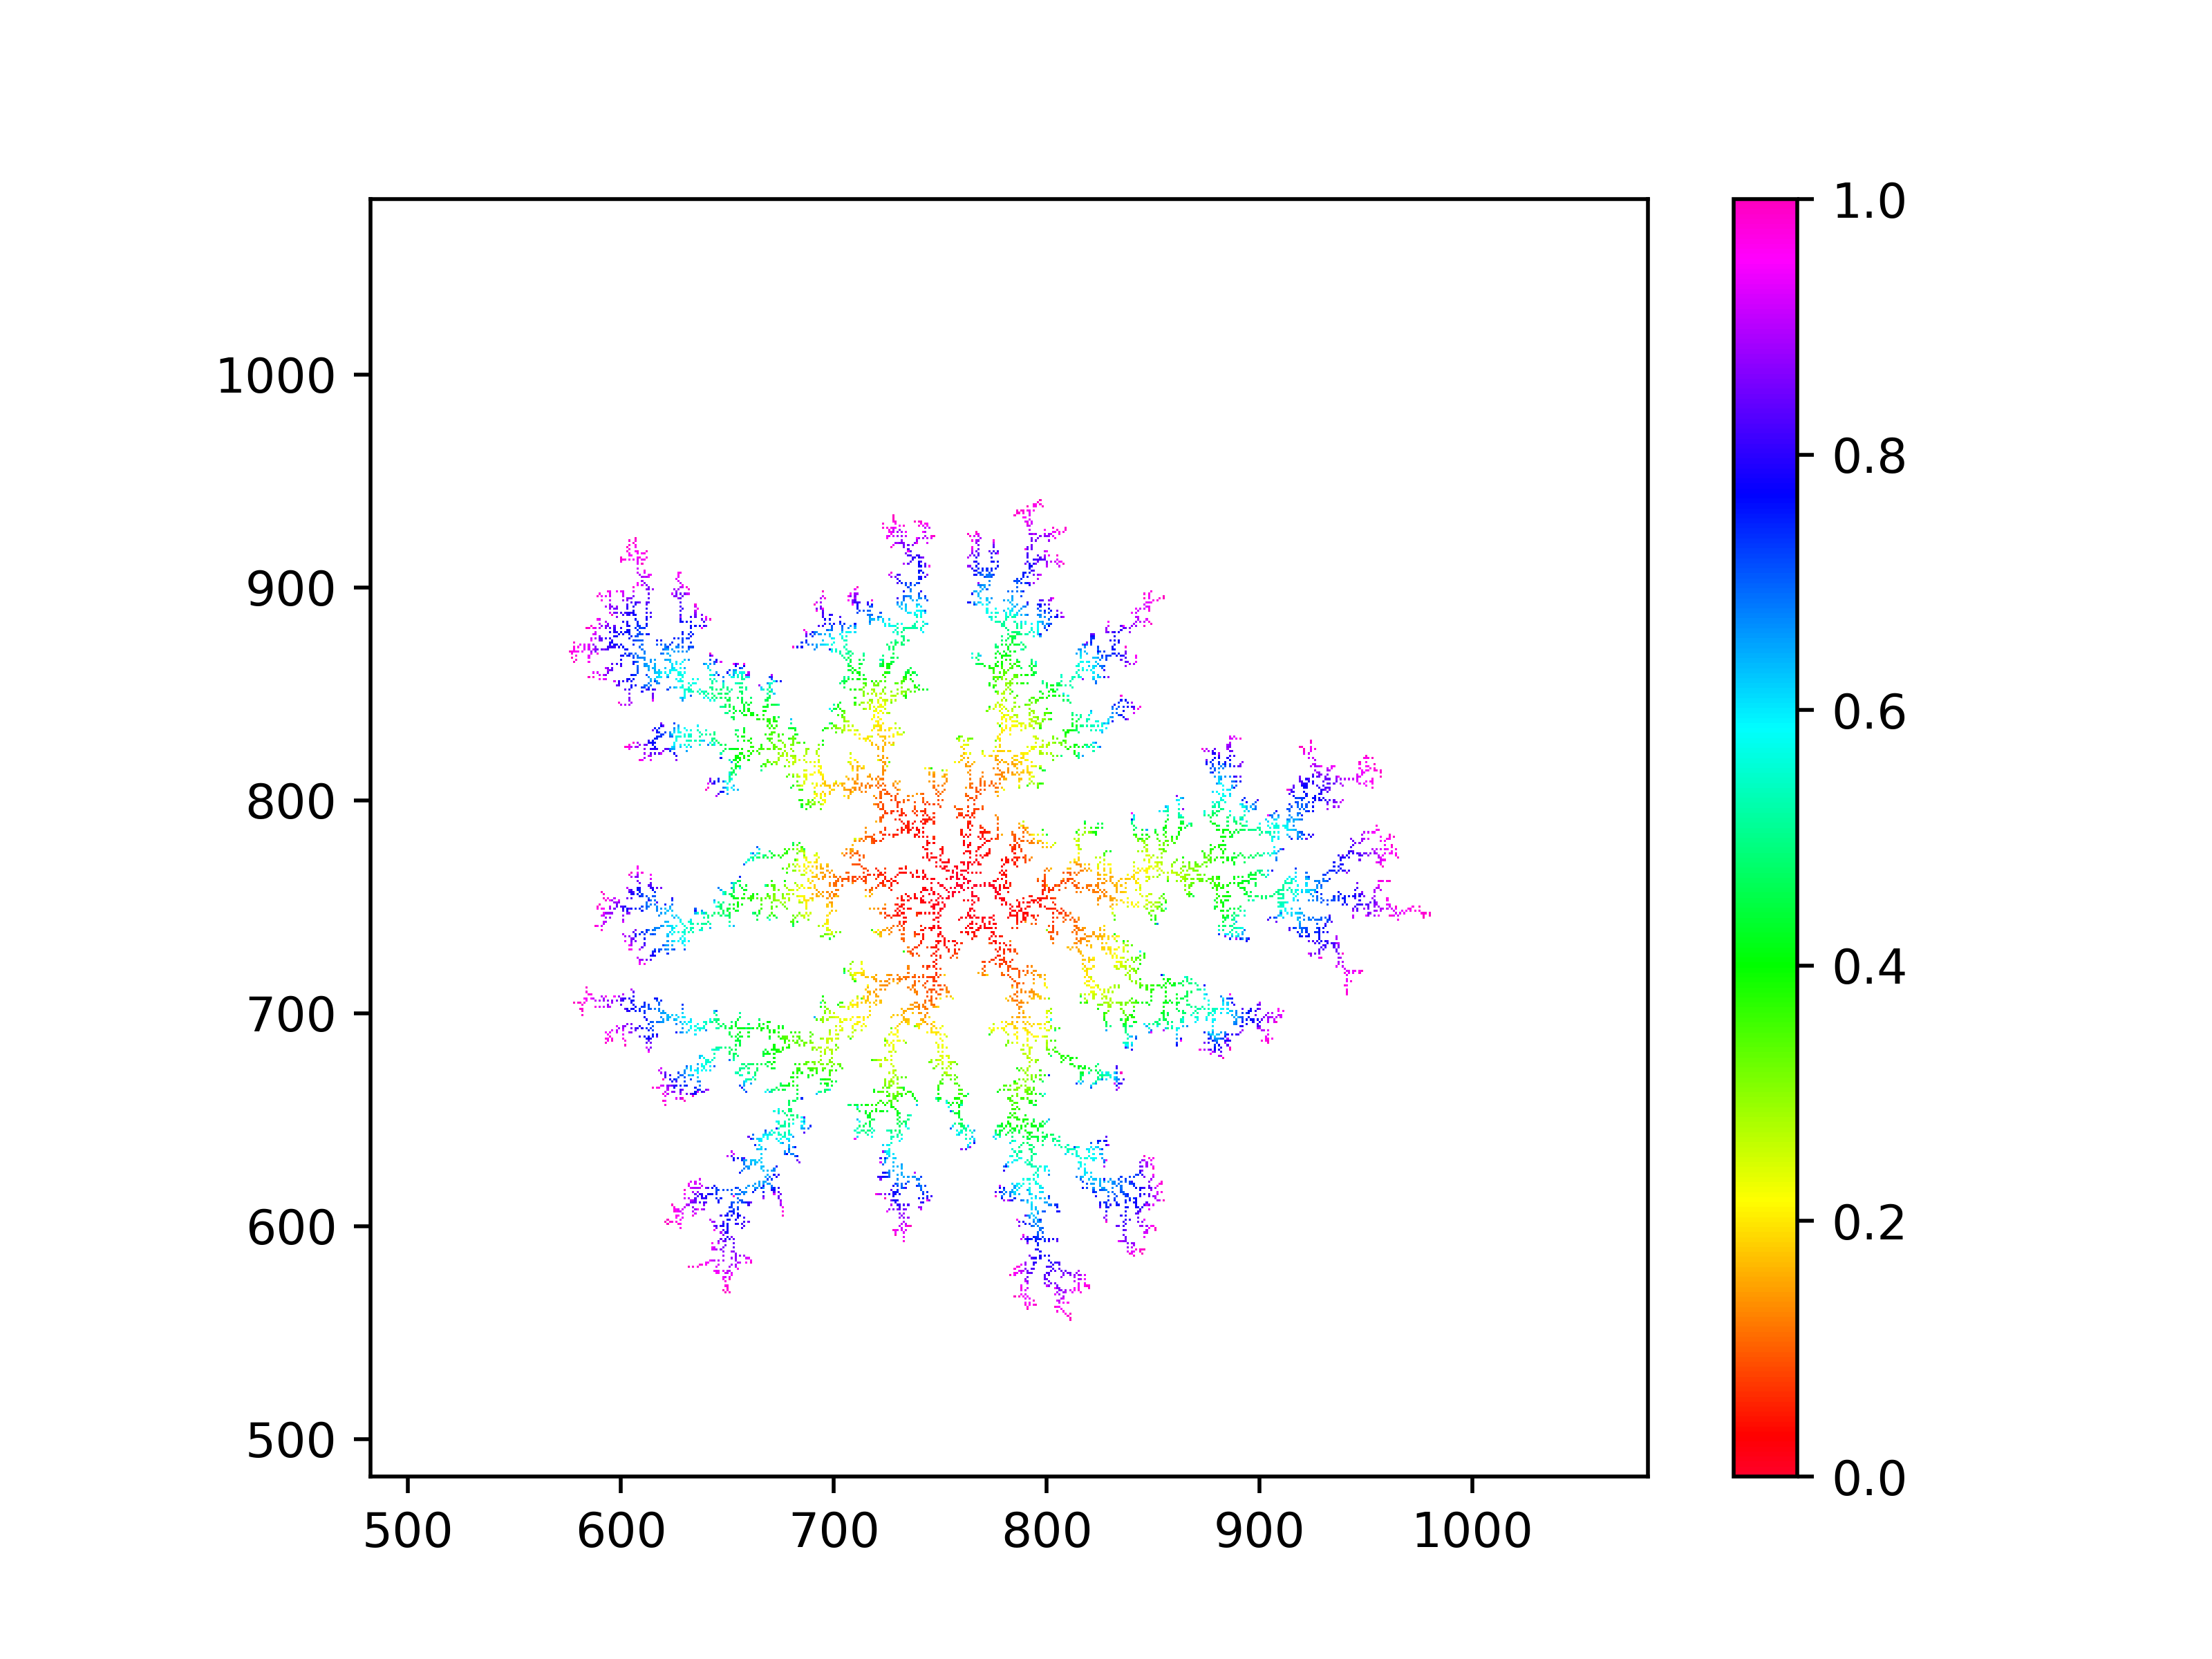
\includegraphics[width=\textwidth]{Figure_13}
		\caption{Adjacent Sticking \#Prob.=30\%, Second Sticking \#Prob.=15\%, clustering rate=80.82\%}
	\end{subfigure}
	\caption{Distant Sticking for Different Probabilities}
\end{figure}

Similarly, we calculated the dimensions for both cases by fitting the cumulative density function $S(r)$ using the corresponding 10 simulations, shown in Figure 9.

\begin{figure}[h]
	\centering
	\begin{subfigure}[b]{0.3\textwidth}
		\centering
		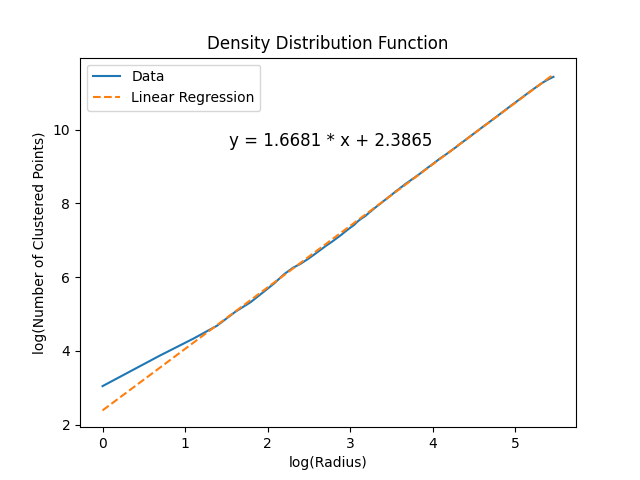
\includegraphics[width=\textwidth]{Figure_8}
		\caption{Density Function $\ln S(r) \text{ vs } \ln r$ for $P_{nn} = 1, P_{snn} = 0.5$}
	\end{subfigure}
	% \hfill
	\begin{subfigure}[b]{0.3\textwidth}
		\centering
		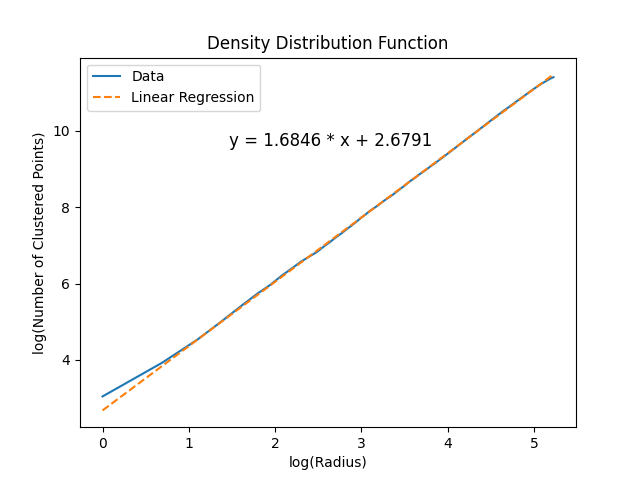
\includegraphics[width=\textwidth]{Figure_9}
		\caption{Density Function $\ln S(r) \text{ vs } \ln r$ for $P_{nn} = 0.3, P_{snn} = 0.15$}
	\end{subfigure}
	\caption{$\ln S(r) \text{ vs } \ln r$ for Different Adjacent \& Distant Sticking Probability}
\end{figure}

The fitting results together with the dimensions obtained from $S(r)$ are listed in the Table 2 below.


\begin{table}[h]
	\begin{center}
	\begin{tabular}{|c|c|c|c|}
		\hline
		\multirow{2}{*}{\shortstack{Adjacent Sticking\\Probability}} & \multirow{2}{*}{\shortstack{Second Nearest\\Sticking Probability}} & \multirow{2}{*}{\shortstack{Slope Obtained\\from $S(r)$}} & \multirow{2}{*}{\shortstack{Dimension\\Obtained from $S(r)$}} \\
		& & & \\
		\hline
		1 & 0.5 & $1.668\pm 0.004$ & 1.668 \\
		\hline
		0.3 & 0.15 & $1.685\pm 0.003$ & 1.685 \\
		\hline
	\end{tabular}
	\caption{Dimensions Obtained from both $C(r)$ \& $S(r)$}
\end{center}
\end{table}

\newpage

\subsection{2-Dimensional with Modified Initial Clustering}

For simplicity, we only gives some of the typical examples of the initial clustering.

\subsubsection{Difference Shapes of the Initial Clustering}

Below in Figure 10 shows the cases for different cases of initial clusterings. We've introduced the boundary sticking condition to the aggregation. Note that the figure on the left obeys the input rules discussed before, where the input is at the radius about the current maximum clustering radius, the figure on the right, on the other hand, simulates for the condition where the input is totally radius with in the given circle. It is obvious and follows the intuition that the dimension of the right figure is larger.

\begin{figure}[h]
	\centering
	\begin{subfigure}[b]{0.3\textwidth}
		\centering
		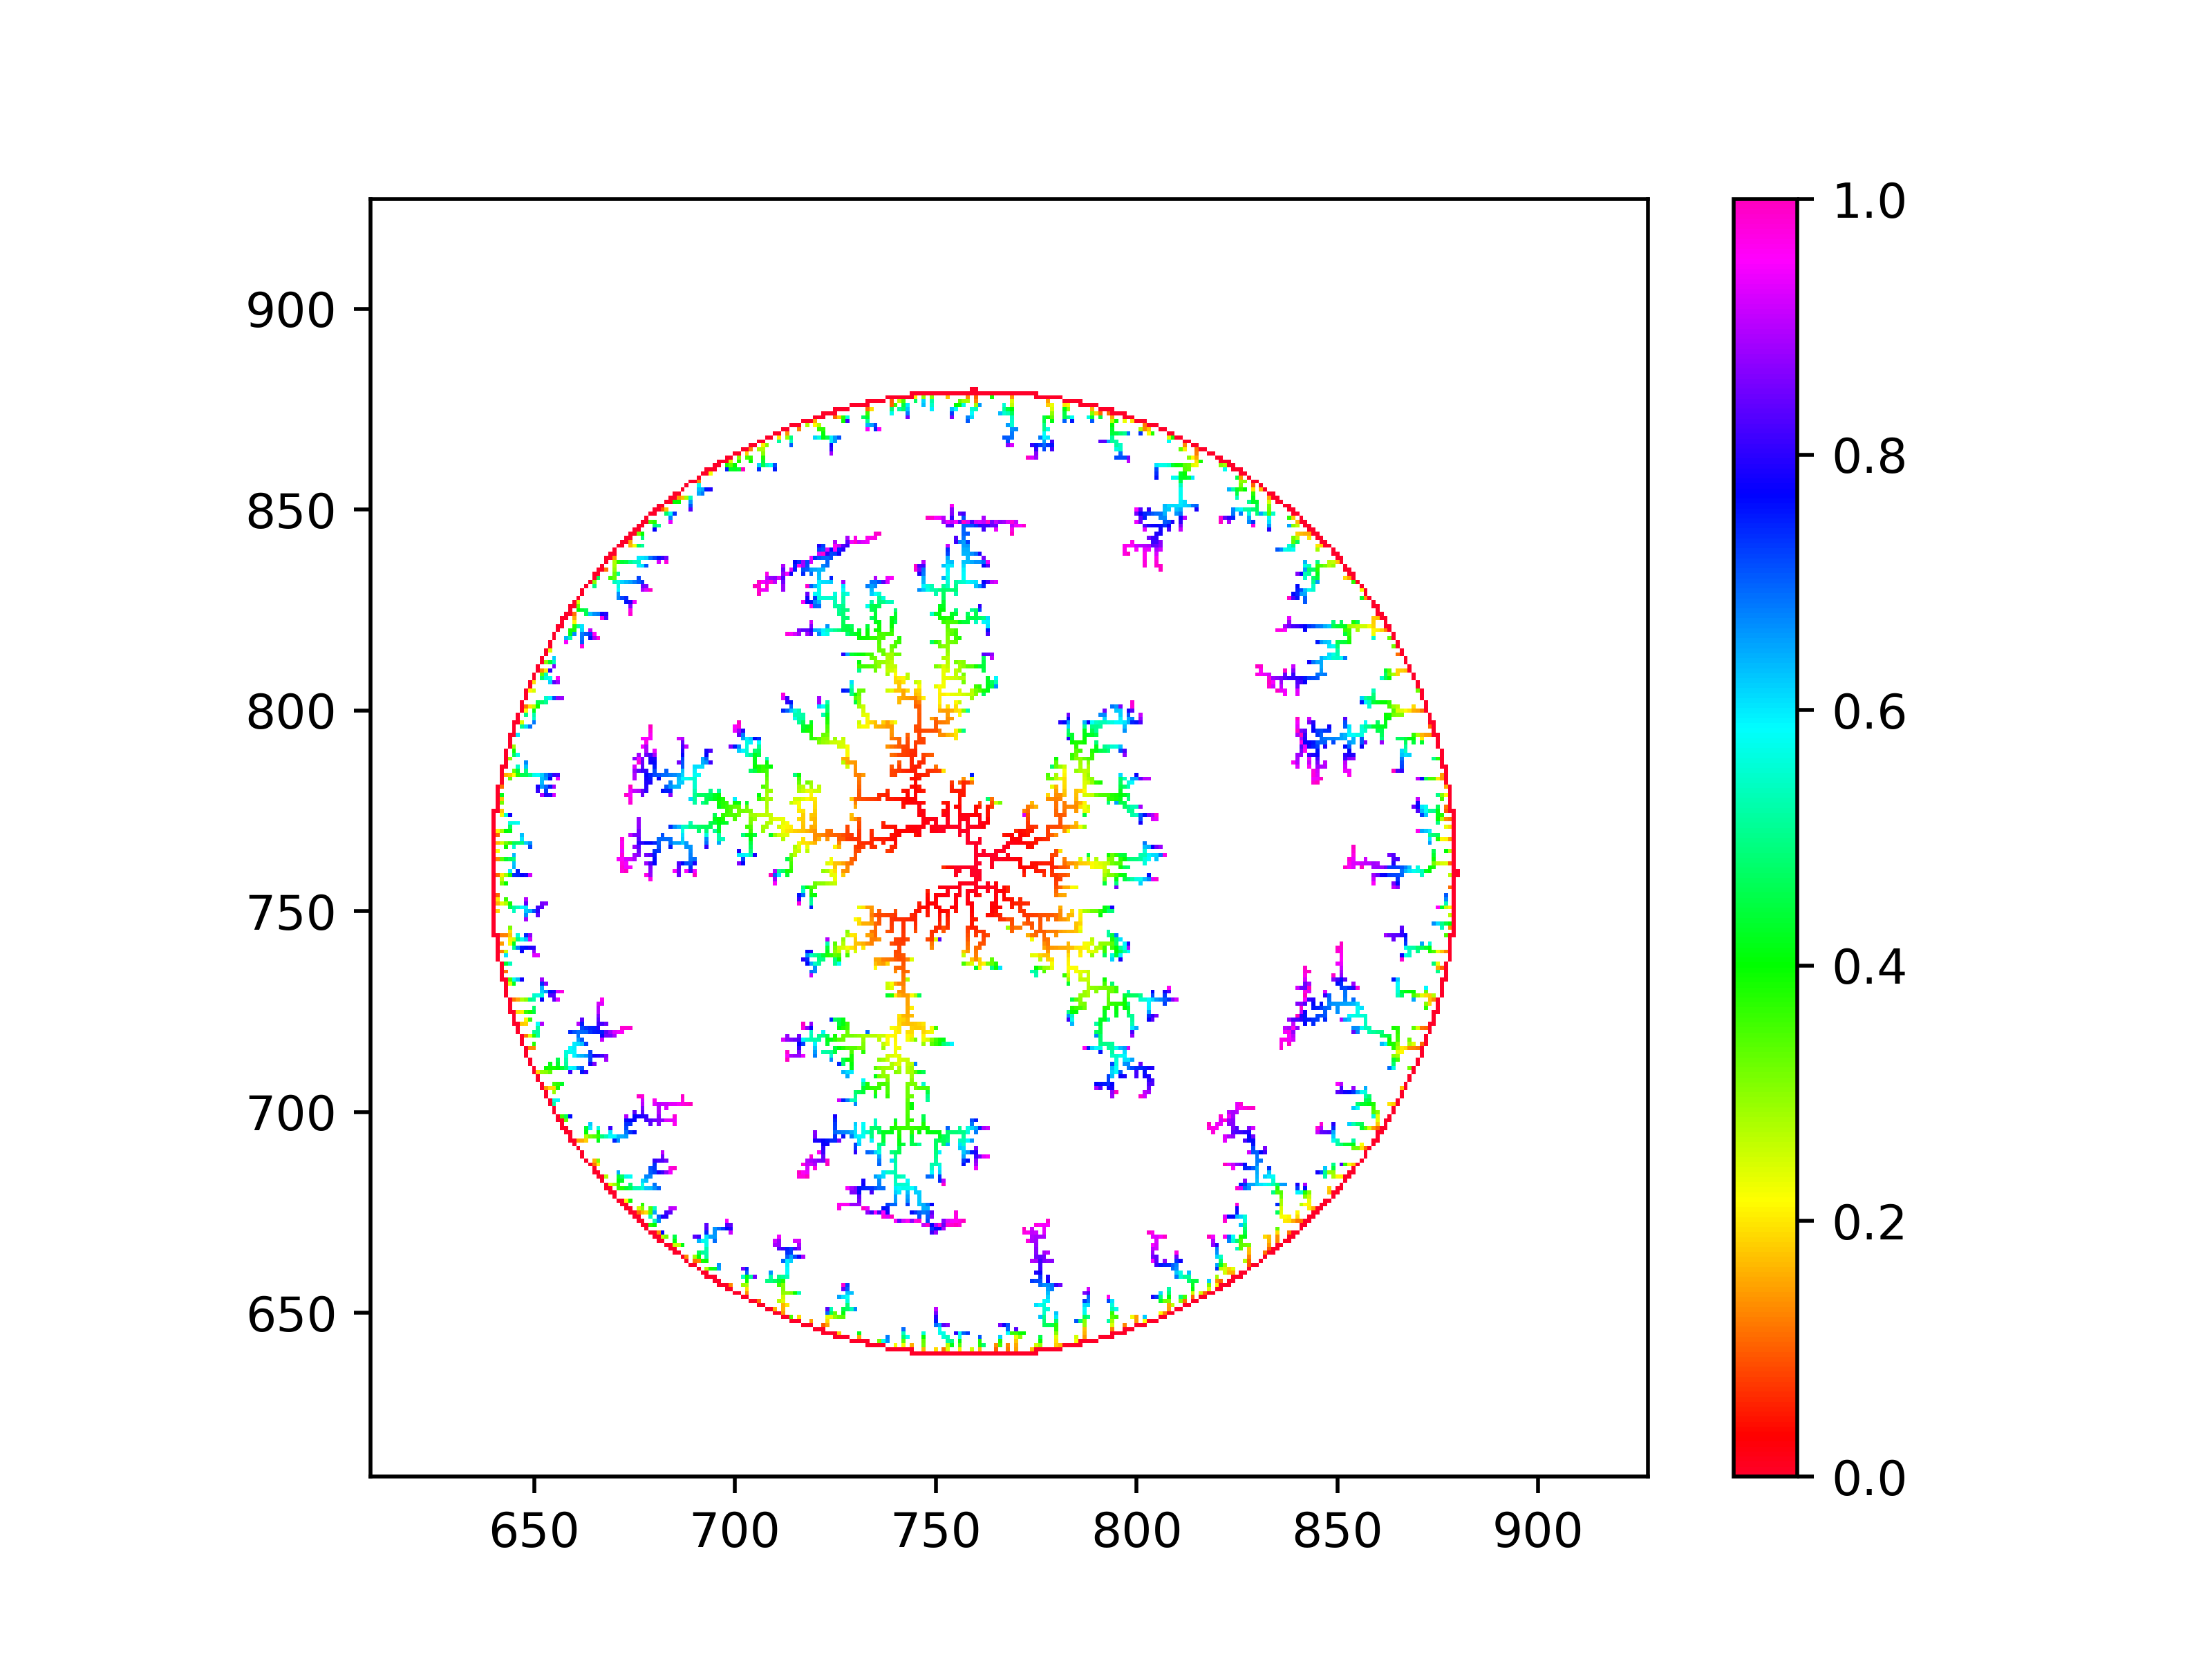
\includegraphics[width=\textwidth]{Figure_14}
		\caption{Input at the Radius about Current Maximum Clustering Radius}
	\end{subfigure}
	% \hfill
	\begin{subfigure}[b]{0.3\textwidth}
		\centering
		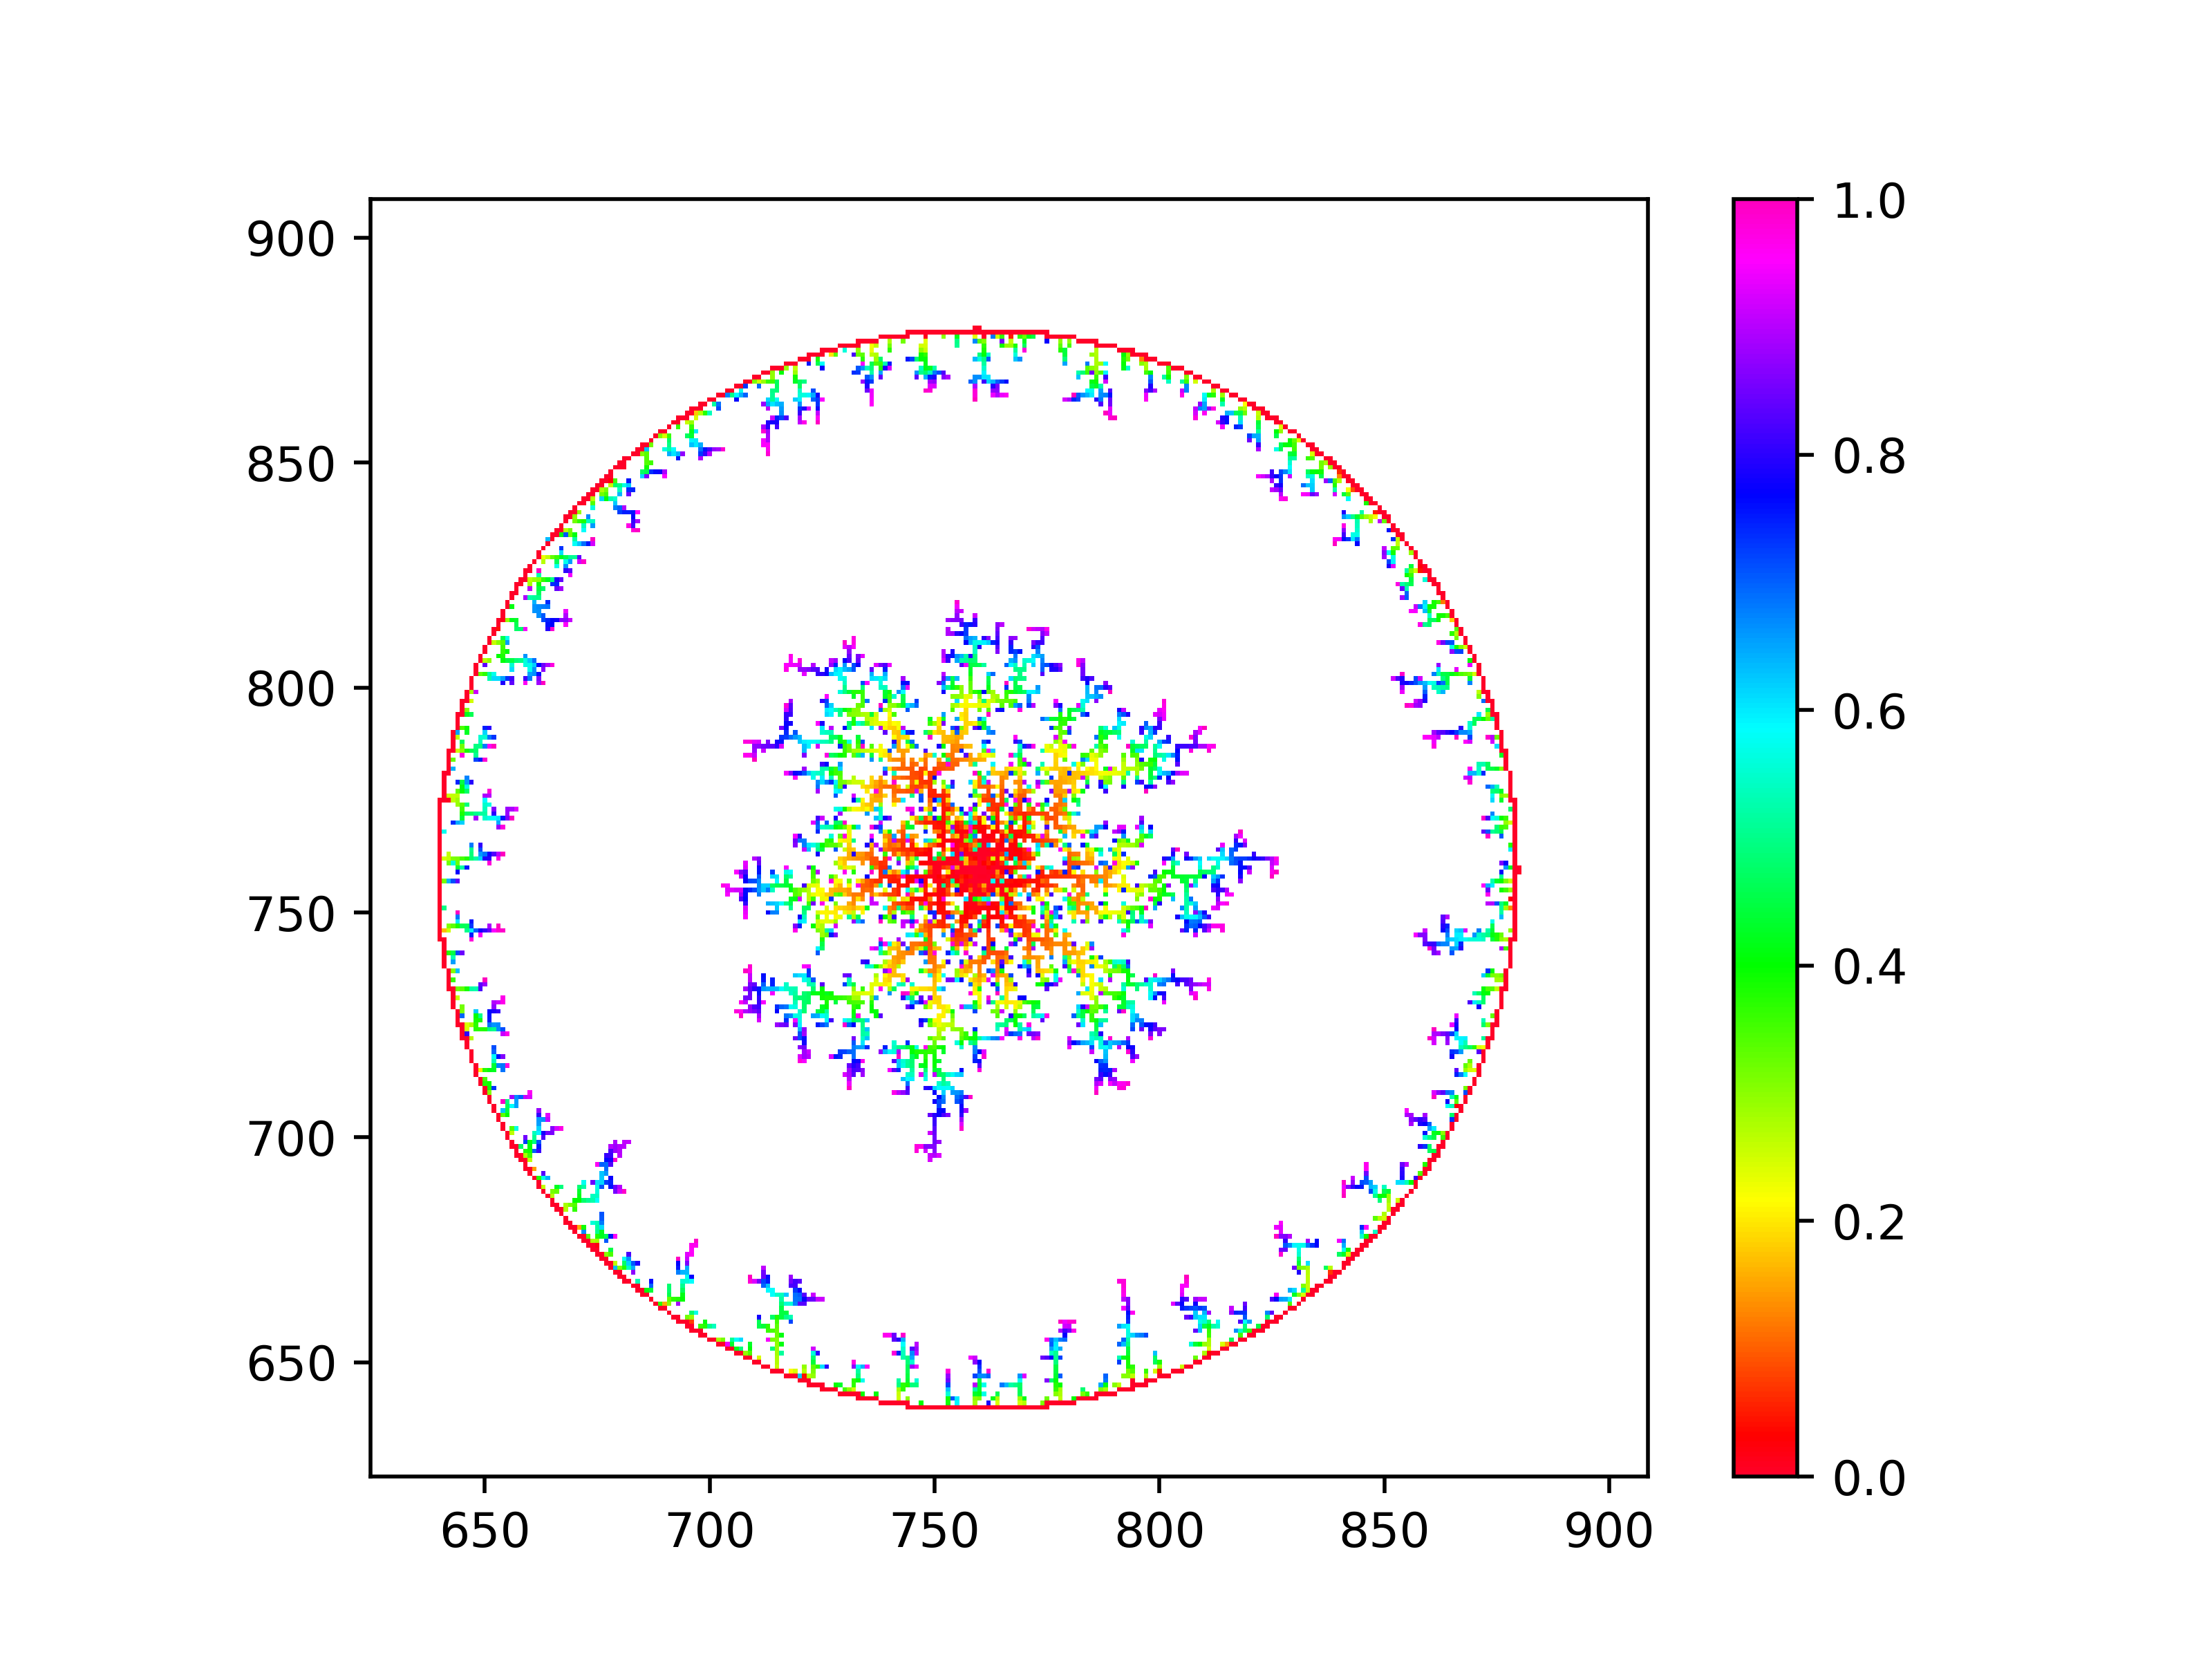
\includegraphics[width=\textwidth]{Figure_15}
		\caption{Input Randomly within the Circle}
		\end{subfigure}
		\caption{Boundary Clusterings for Circle}
\end{figure}

Next, we show how the initial condition affects the aggregation results. For simplicity, we set the initial cluster as a circle and let the cluster grow outside the circle. The result is stored inside the folder \texttt{Other\_Simulation/Modified\_Boundary}. The sample results are shown in Figure 11 below.

\begin{center}
	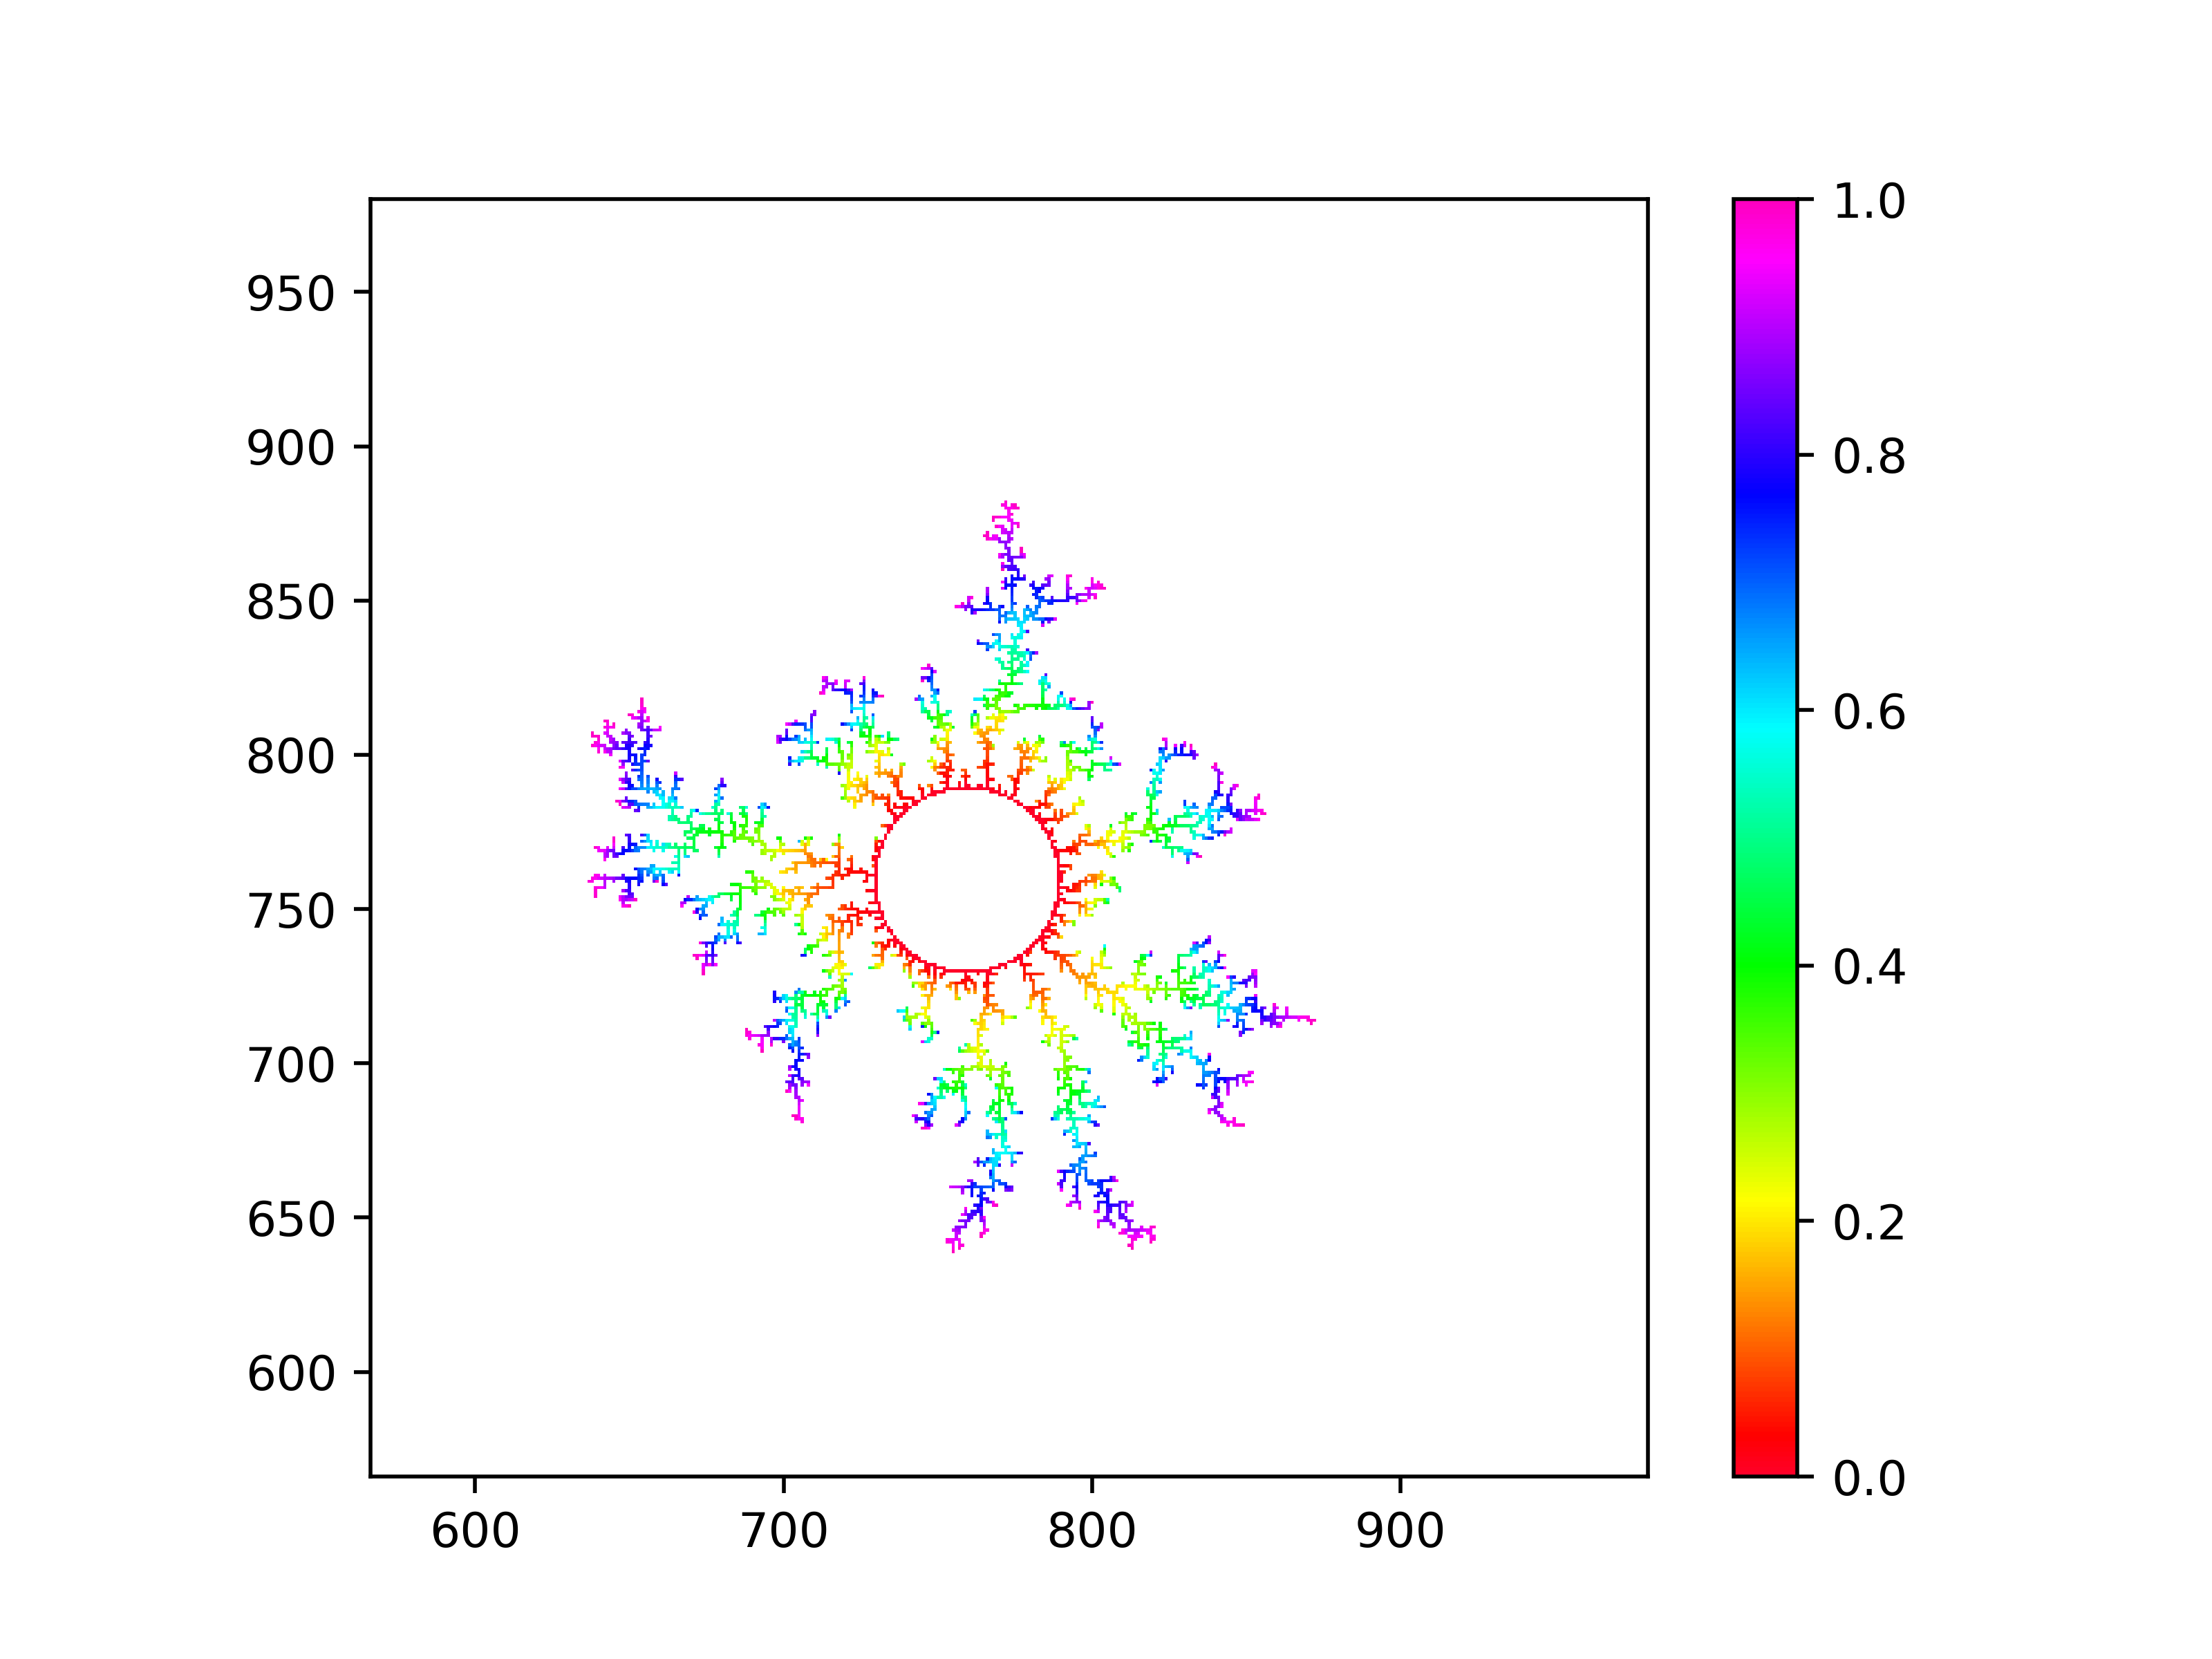
\includegraphics[width=0.4\textwidth]{Figure_16}
	\captionof{figure}{Initial Condition as a Circle}
\end{center}

Similarly, we fitted the dimension using linear approximation over 5 aggregation results, with the fitting result shown in Figure 17 below.

\begin{center}
	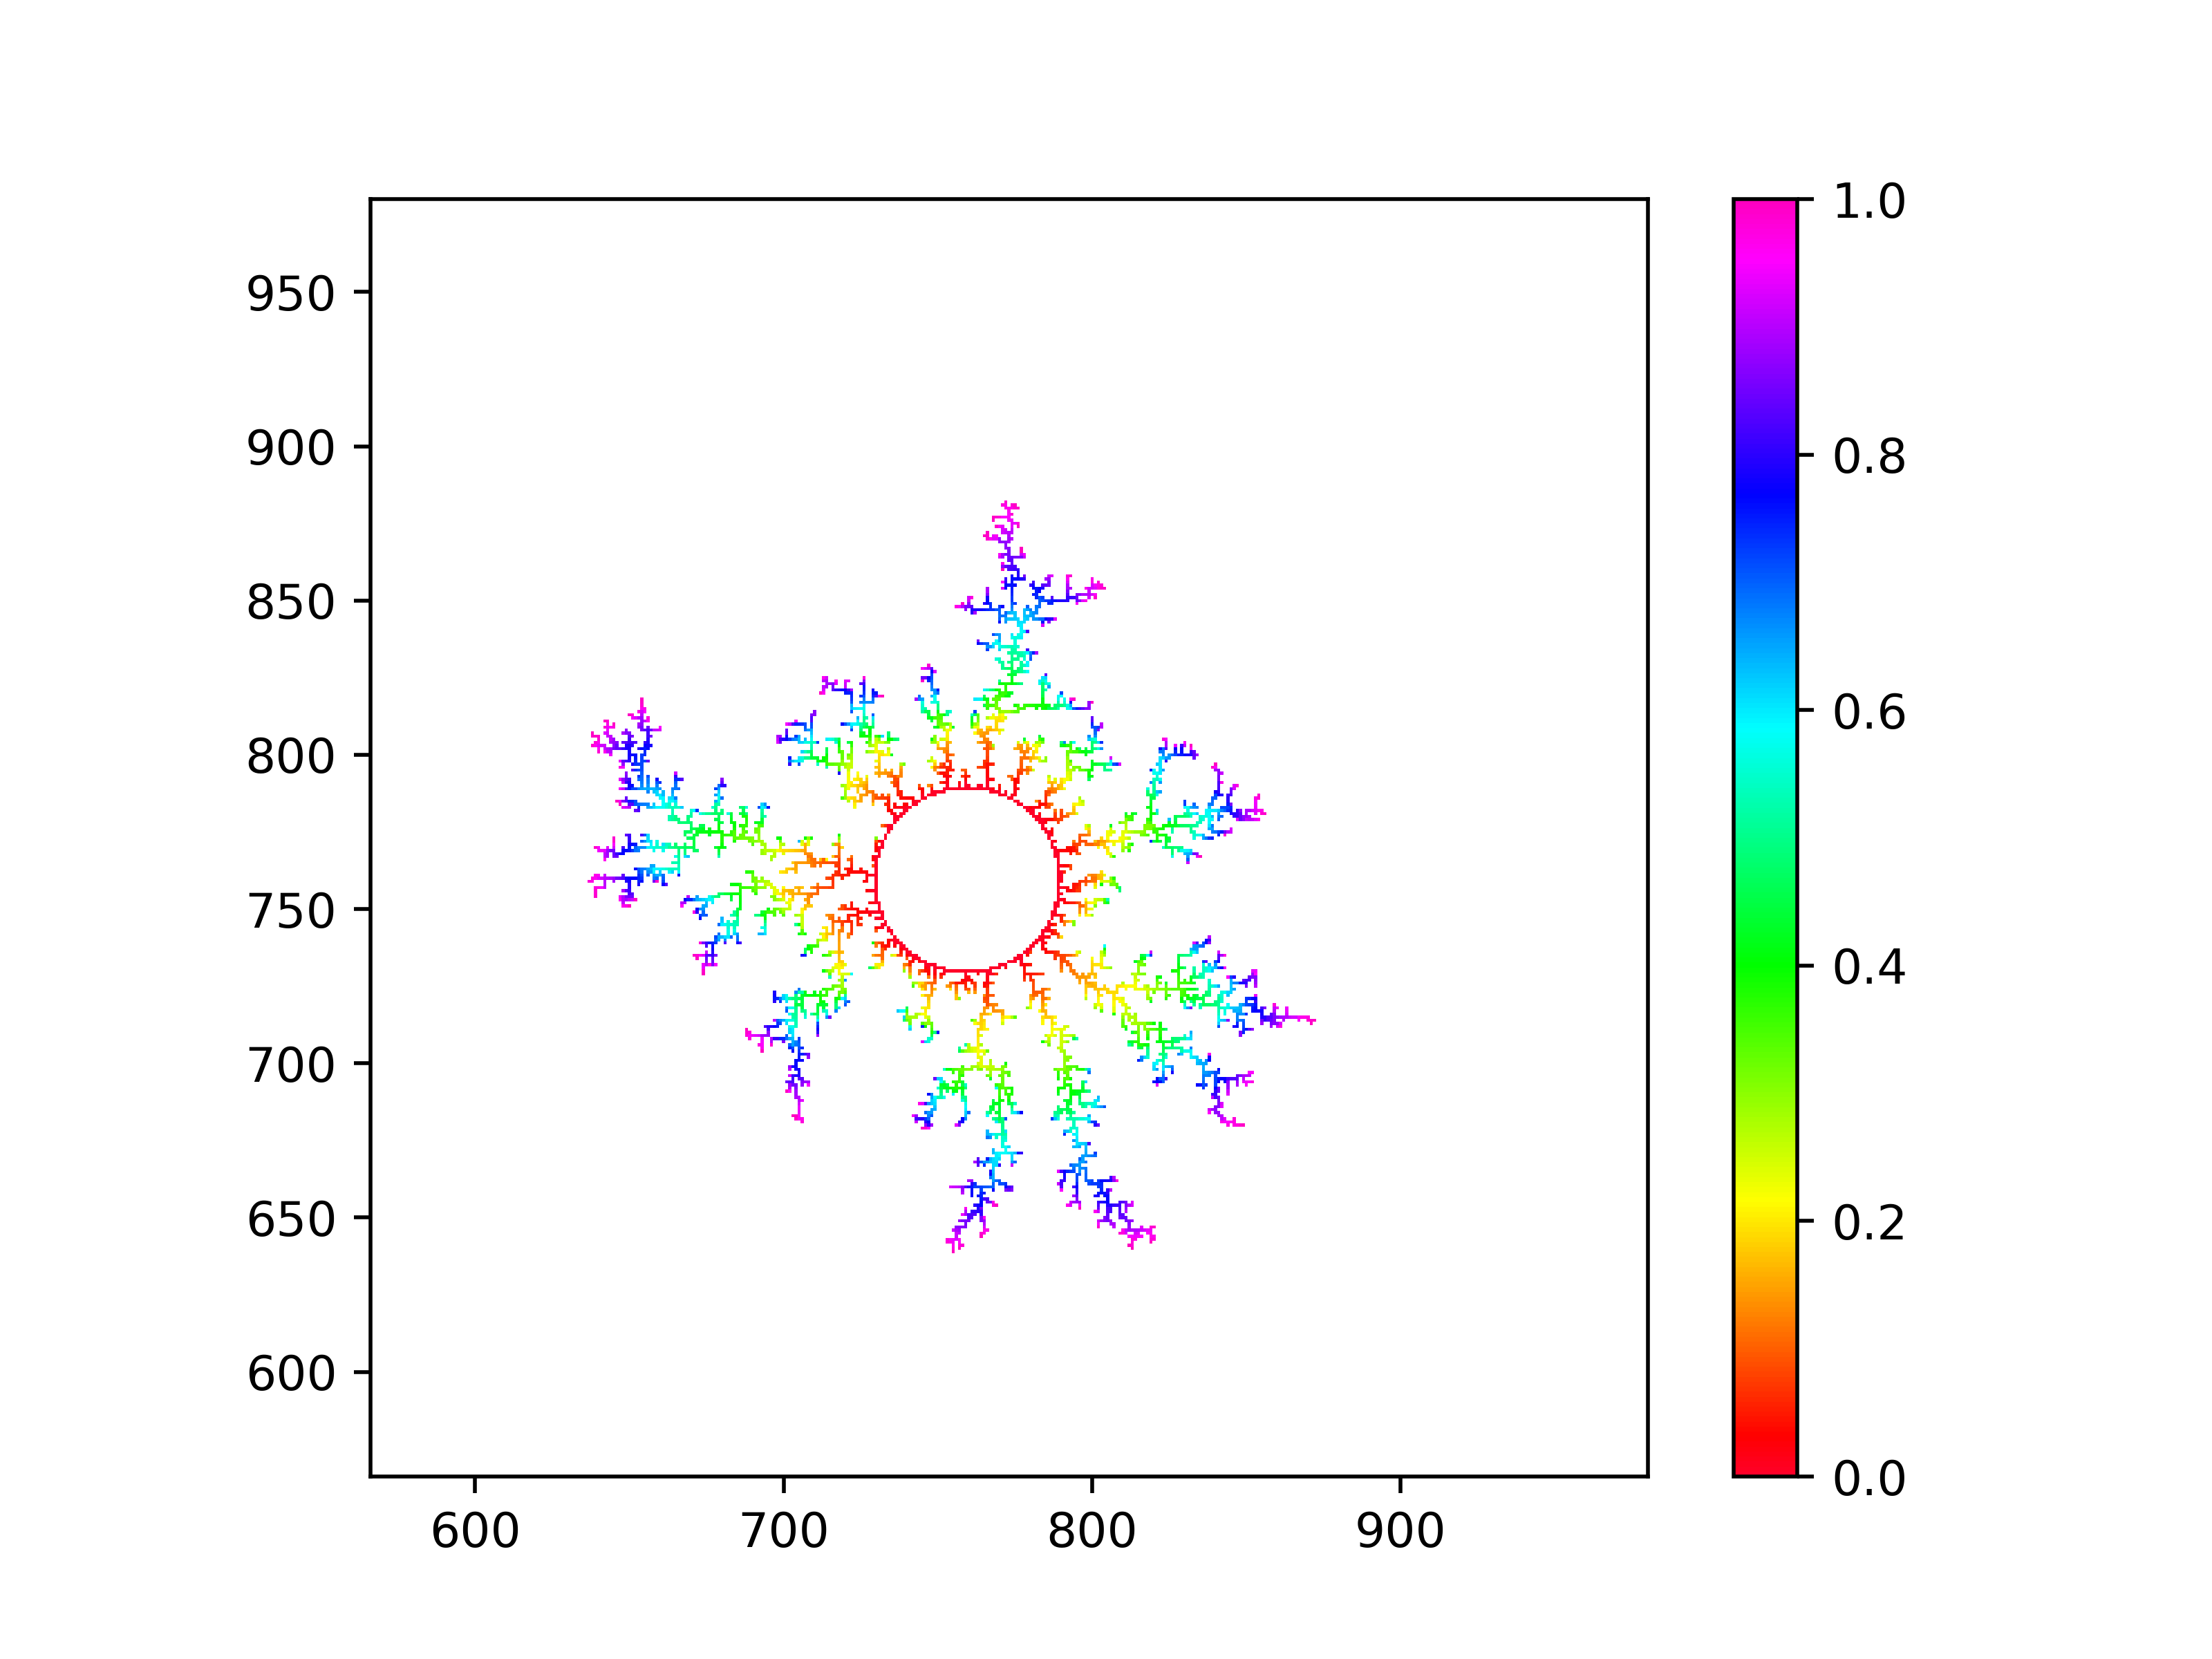
\includegraphics[width=0.4\textwidth]{Figure_16}
	\captionof{figure}{Dimension of the Circular Initial Condition}
\end{center}

%\subsubsection{Multiple Initial Clusterings}

\subsection{2-Dimensional with Inconsistent Probability to Differernt Directions}

In this section, we modify the probability of the random walking. For simplicity, we only consider the two cases specified as below.

\subsubsection{$P_{down} = 0.1$, $Others = 0.3$}

Figure below shows the example of the $P_{down} = 0.1$, $Others = 0.3$.

\begin{center}
	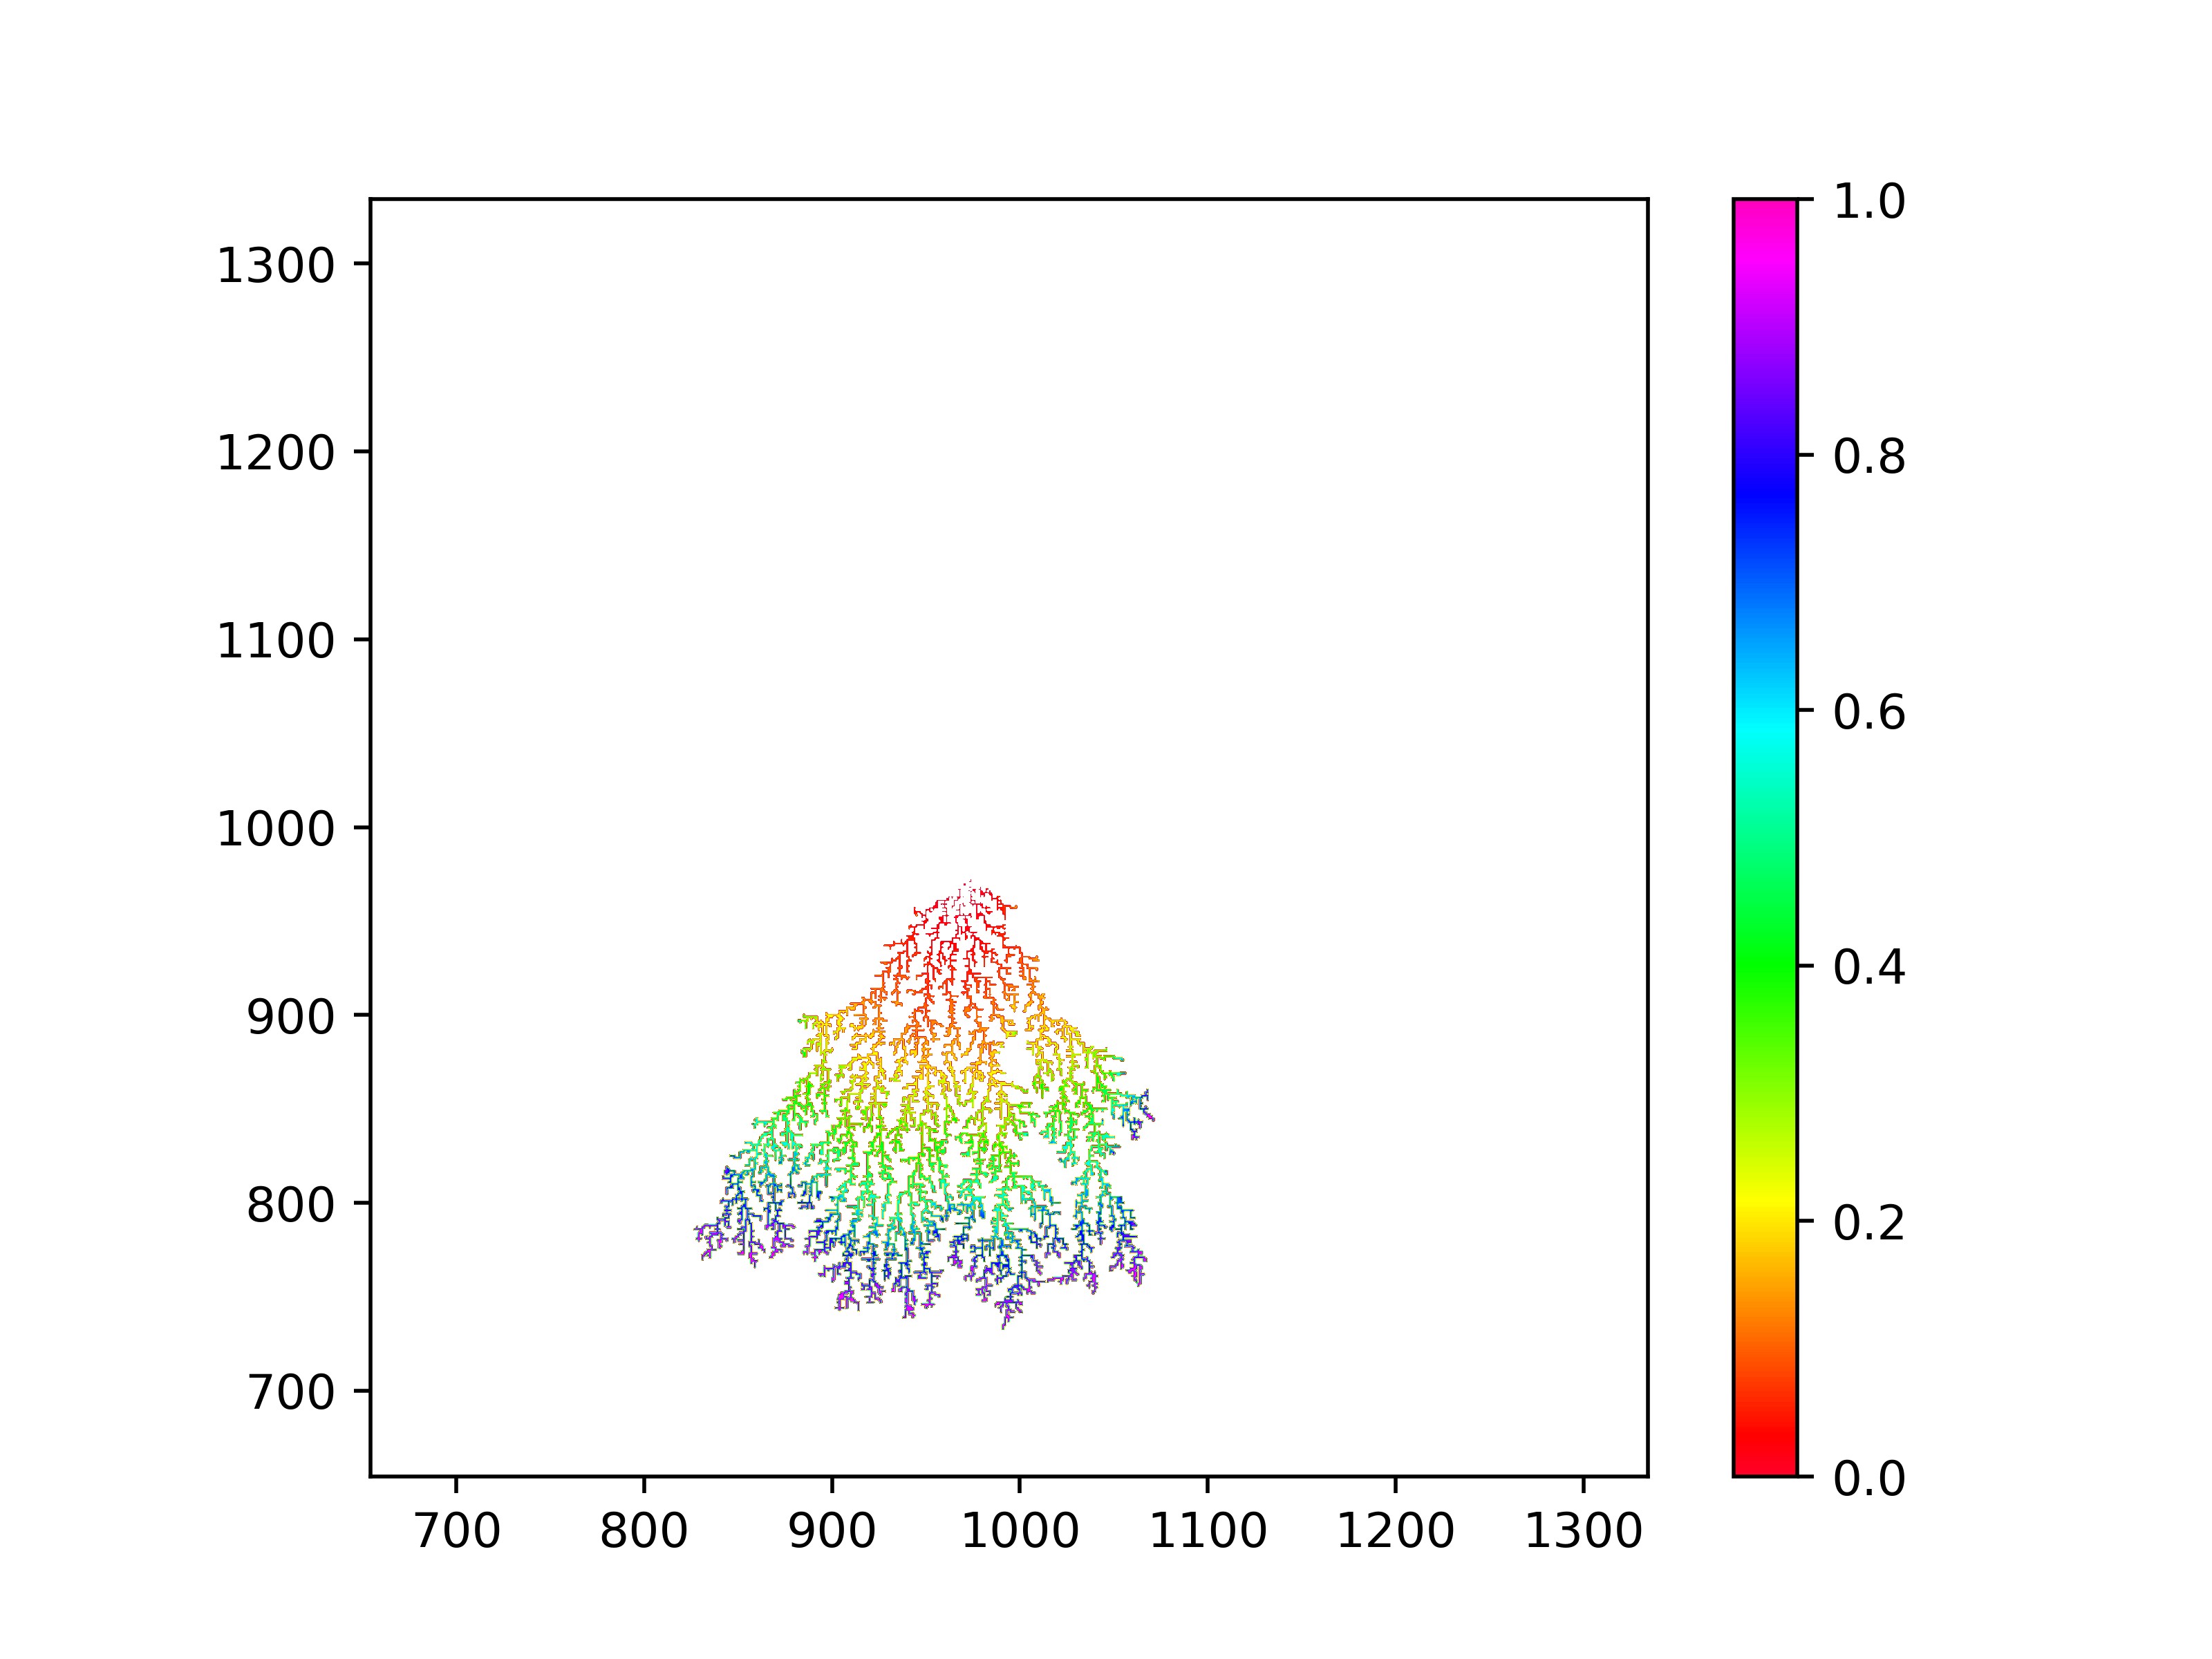
\includegraphics[width=0.4\textwidth]{Figure_19}
	\captionof{figure}{Simulation of the DLA $P_{down} = 0.1$, $Others = 0.3$}
\end{center}

\subsubsection{$P_{up \& down} = 0.1$, $Others = 0.4$}

Figure below shows the example of the $P_{down} = 0.1$, $Others = 0.3$.

\begin{center}
	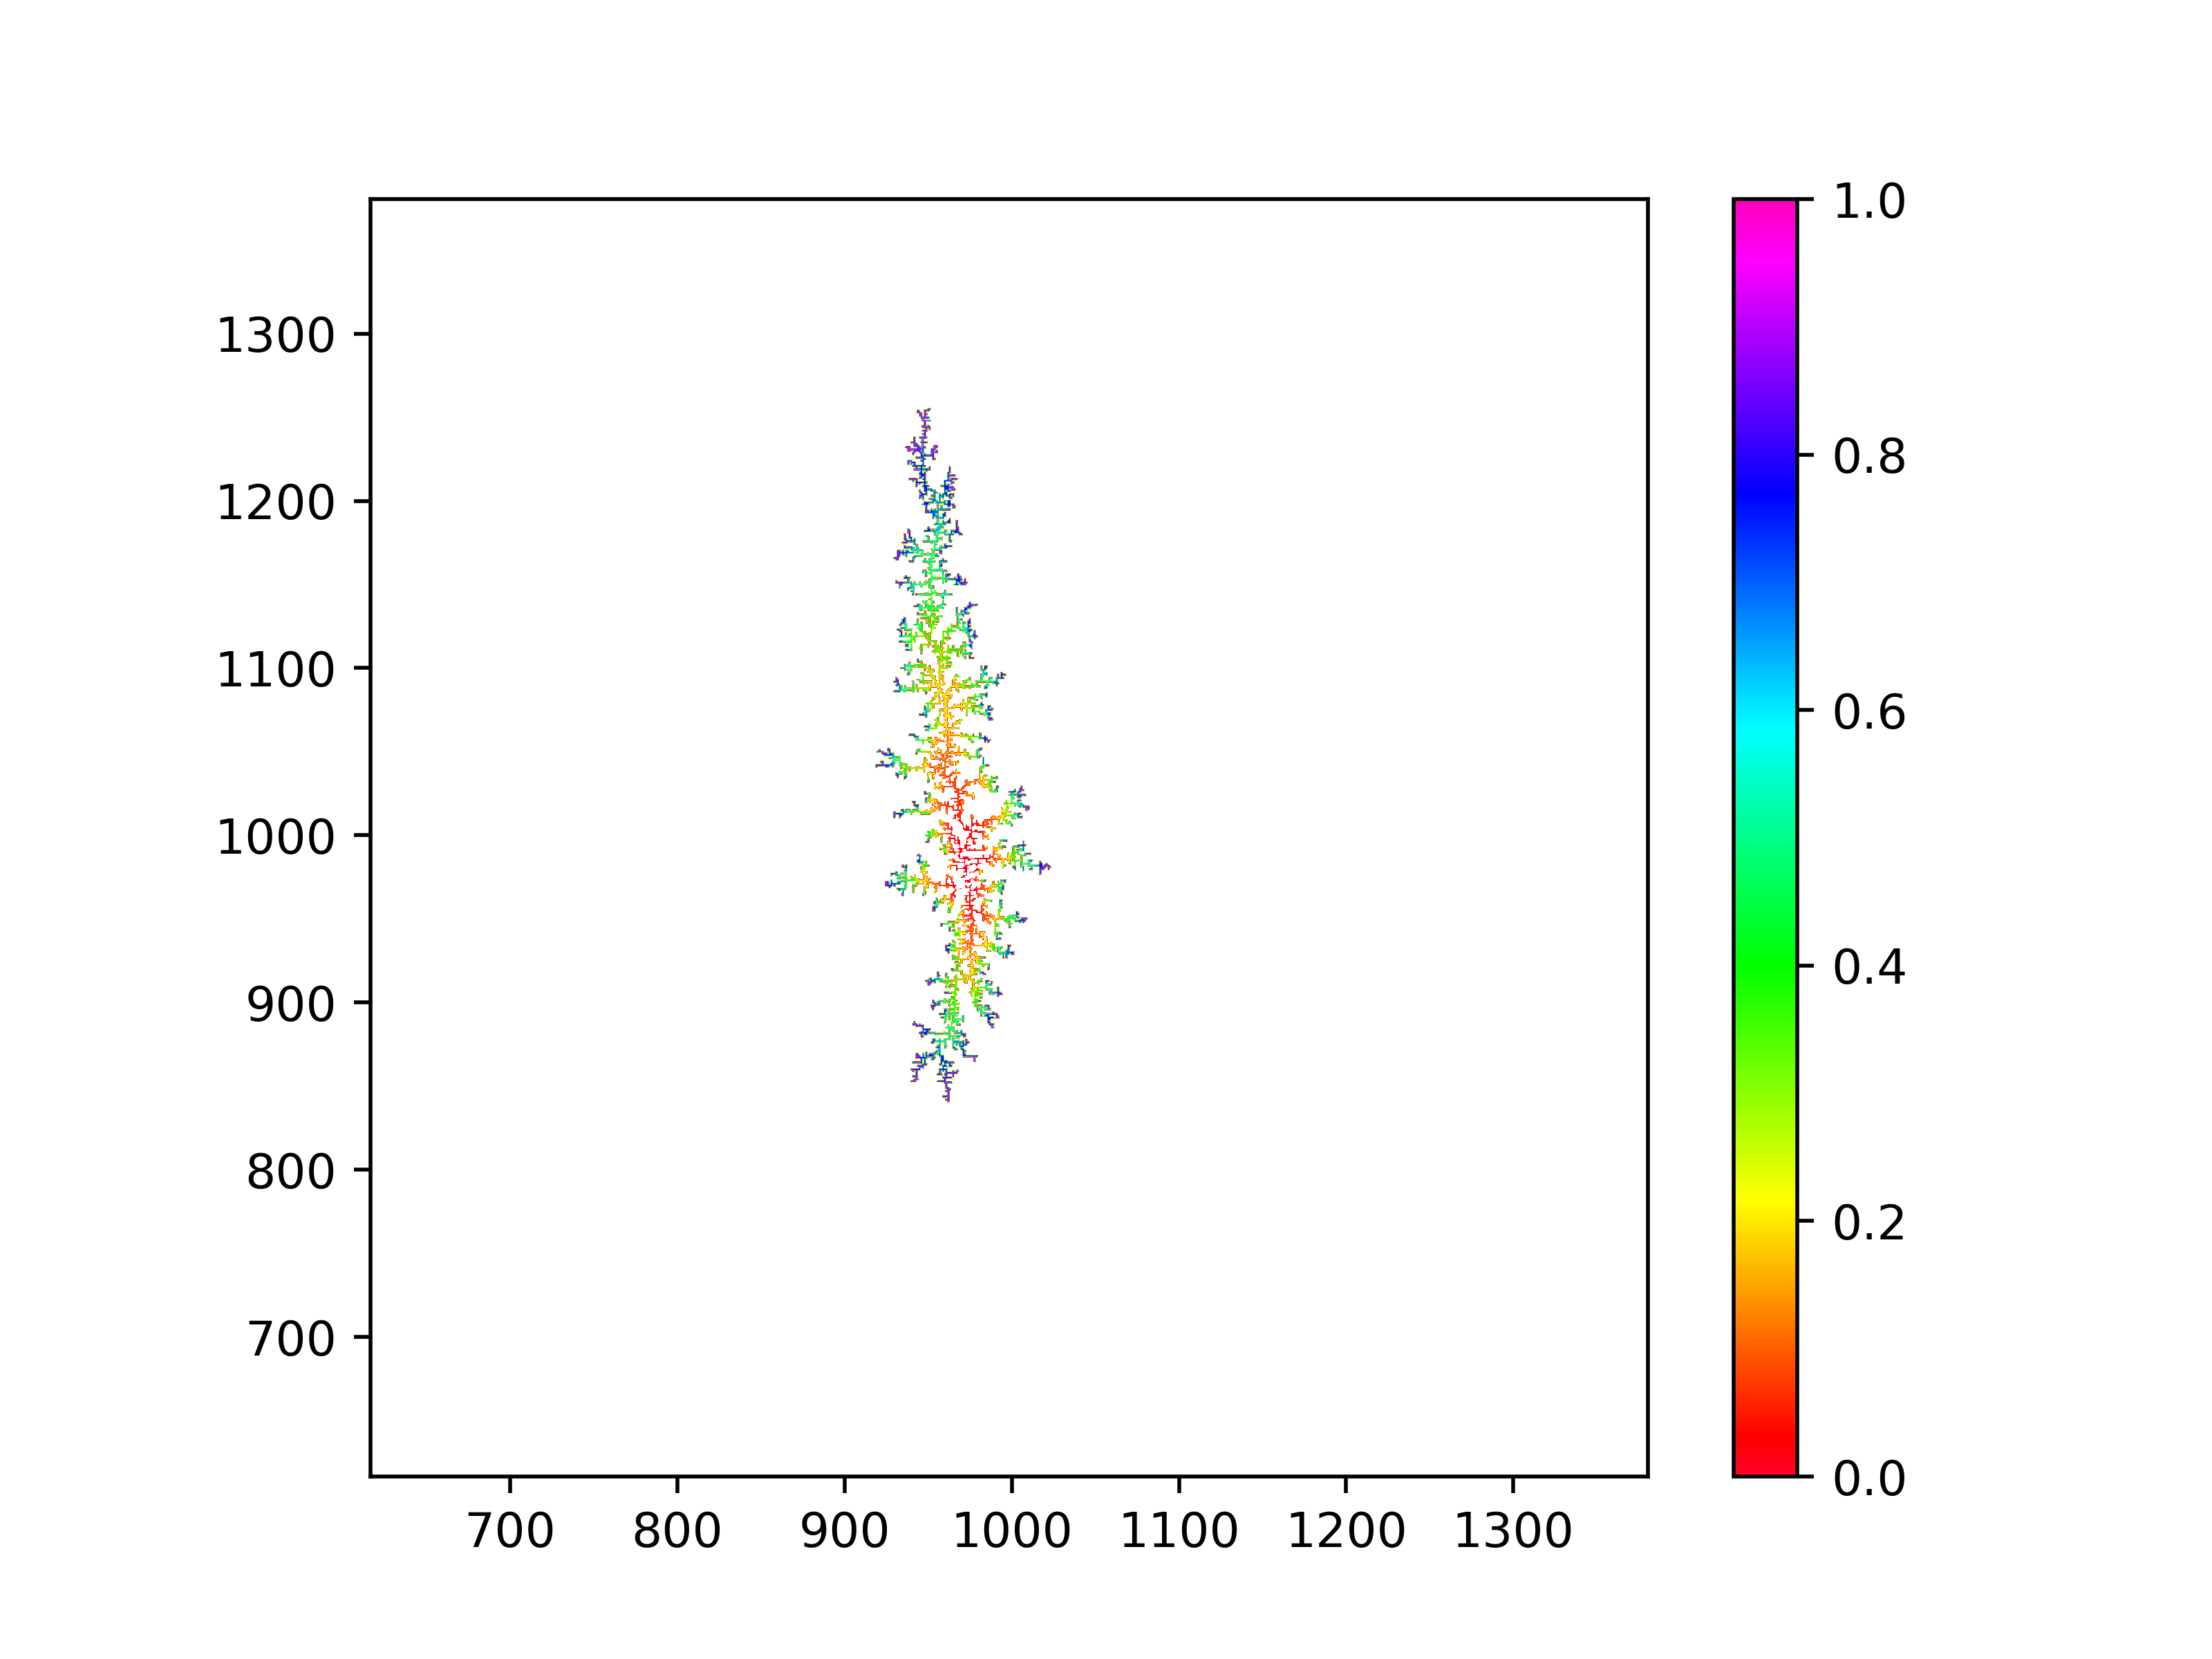
\includegraphics[width=0.4\textwidth]{Figure_20}
	\captionof{figure}{Simulation of the DLA $P_{up \& down} = 0.1$, $Others = 0.4$}
\end{center}

%\subsection{3-Dimensional Simulation}

\section{Simulation of the DLA in Triangular Lattice}

Below shows a rough result of the simulation in a triangular lattice.

\begin{center}
	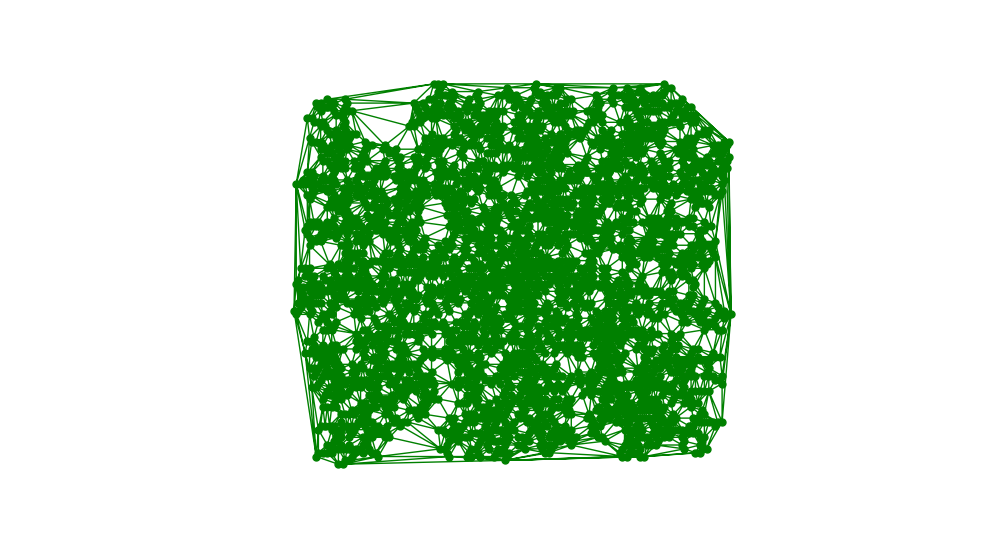
\includegraphics[width=0.4\textwidth]{Figure_18}
	\captionof{figure}{Simulation of the DLA in Triangular Lattice}
\end{center}

%\section{Simulation of the DLA in Hexagonal Lattice}

%\section{Simulation with the Interaction between Particles is Considered}

%\section{Results and Discussion}

%\section{Conclusion}

\newpage

\section{References}

\label{ref1}
[1] "Diffusion-limited aggregation" Wikipedia. Available at \href{https://en.wikipedia.org/wiki/Diffusion-limited_aggregation}{https://en.wikipedia.org/wiki/Diffusion-limited\_aggregation}

\label{ref2}
[2] "Diffusion-Limited Aggregation" by T.A. Witten and L.M. Sander (1981). Available at\\ \href{https://journals.aps.org/prb/abstract/10.1103/PhysRevB.27.5686}{https://journals.aps.org/prb/abstract/10.1103/PhysRevB.27.5686}

\label{ref3}
[3] "Diffusion-limited aggregation with multiple point sources" by P. Meakin (1983). Available at\\ \href{https://journals.aps.org/prl/abstract/10.1103/PhysRevLett.51.1119}{https://journals.aps.org/prl/abstract/10.1103/PhysRevLett.51.1119}

\label{ref4}
[4] "Stochastic Models of Diffusion-Limited Aggregation" by S. Redner (1991)

\label{ref5}
[5] "Anisotropic Diffusion-Limited Aggregation" by J. Talbot et al. (1991)

\label{ref6}
[6] "Restricted Diffusion-Limited Aggregation in Two Dimensions" by D. Wilkinson and J.F. Willemsen (1983)

\label{ref7}
[7] PHYS3142 Final project description. Project 2: Diffusion-limited aggregation

\end{document}